\documentclass[10pt,aspectratio=43]{beamer}

\usepackage{graphicx}
\usepackage{tikz}
\usepackage{xcolor}
\usepackage{caption}
\usepackage{subcaption}
\usepackage{bm}
\usetikzlibrary{calc} 
\usepackage{hyperref}
\hypersetup{
    colorlinks=true,
    linkcolor=blue,
    urlcolor=red
}
\usepackage{fontawesome5}
\usepackage{ulem}
\usepackage[dvipsnames]{xcolor}

\usetheme{MyStyle}   % loads beamerthemeMyStyle.sty
\setlength{\columnsep}{0pt}


%%%%%%%%%%%%%%%%%%%%%%%%%%%%%%%%%%%%%%%%%%
%%%%%%%%%%%%%%%%%%%%%%%%%%%%%%%%%%%%%%%%%%
%%%%%%%%%%%%%%%%%%%%%%%%%%%%%%%%%%%%%%%%%%

\title{Coherent DVCS off $^4\mbox{He}$ \\with ALERT}
\newcommand{\eventname}{ALERT meeting}
\author{Felix Touchte Codjo}
\institute{IJCLab}
\date{November 11, 2026}


\begin{document}

\begin{frame}[plain] % remove header, footer, barre de navigation
\titlepage
\end{frame}

%\begin{frame}{Outline}
%\tableofcontents
%\end{frame}

%\section{Intro}
%\section{Updates}

\begin{frame}{Introduction}
    \begin{itemize}
        \item This preliminary work intends to measure the coherent DVCS off $^4\mbox{He}$ within the ALERT experiment
        \item This process gives access to the quark GPDs inside the $^4\mbox{He}$ nucleus
        \item The first step of this analysis is to extract the Beam Spin Asymmetry (BSA) which is related to the Compton Form Factor $\mathcal{H}_{A}$
            \[
                A_{LU} = \frac{1}{P_B} \cdot \frac{N^{+} - N^{-}}{N^{+} + N^{-}}
            \]
        
        \item In the following slides, I describe the process to select DVCS events and I present a preliminary BSA extraction
    \end{itemize}

    % \begin{align*}
    %     A_{LU} &= \frac{1}{P_B} \cdot \frac{N^{+} - N^{-}}{N^{+} - N^{-}} \\
    % \end{align*}

    \centering
    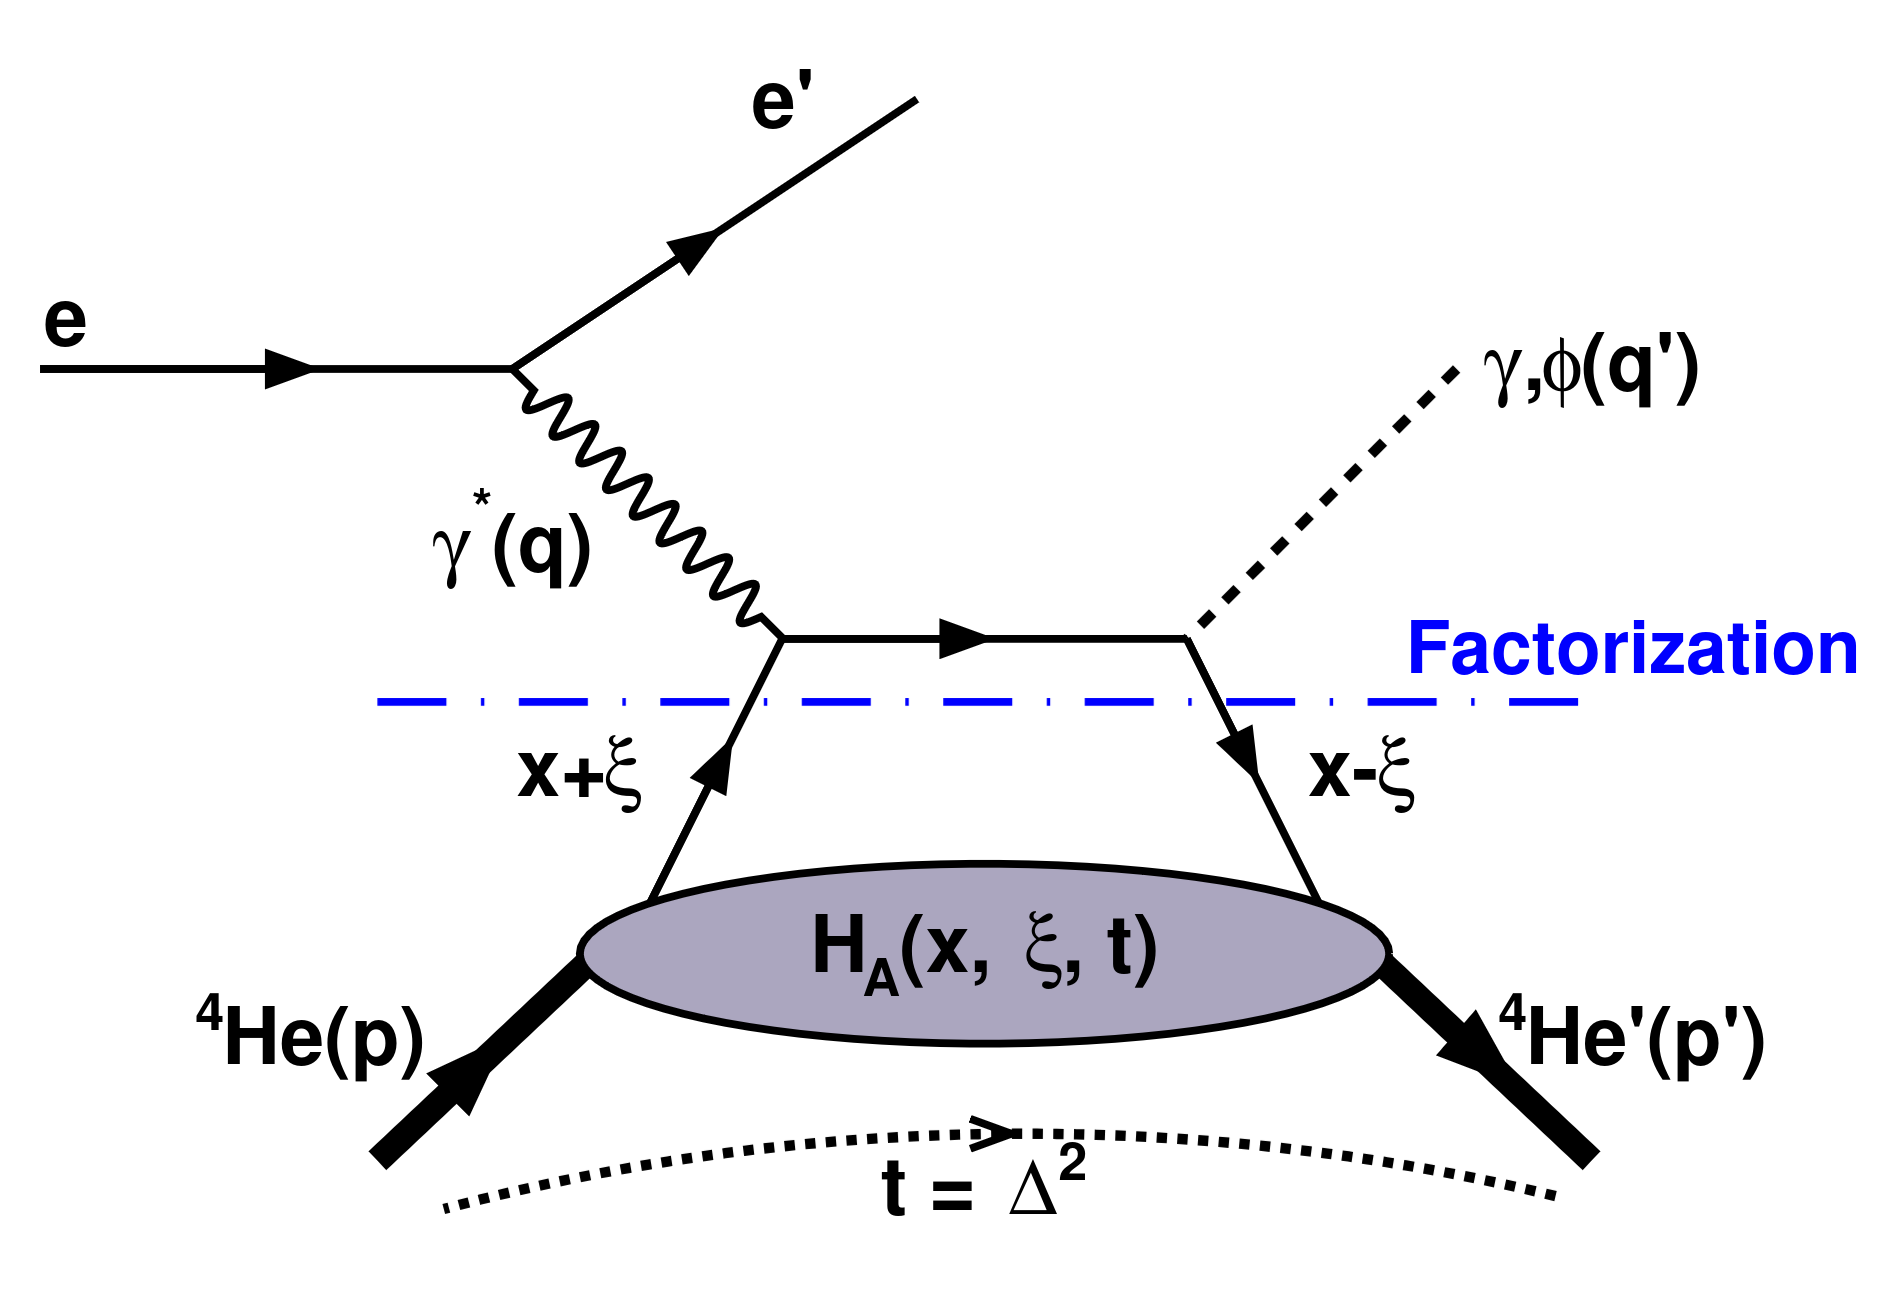
\includegraphics[width=0.4\linewidth]{figures/feynman_diagram.png}
    \hspace{0.4cm}
    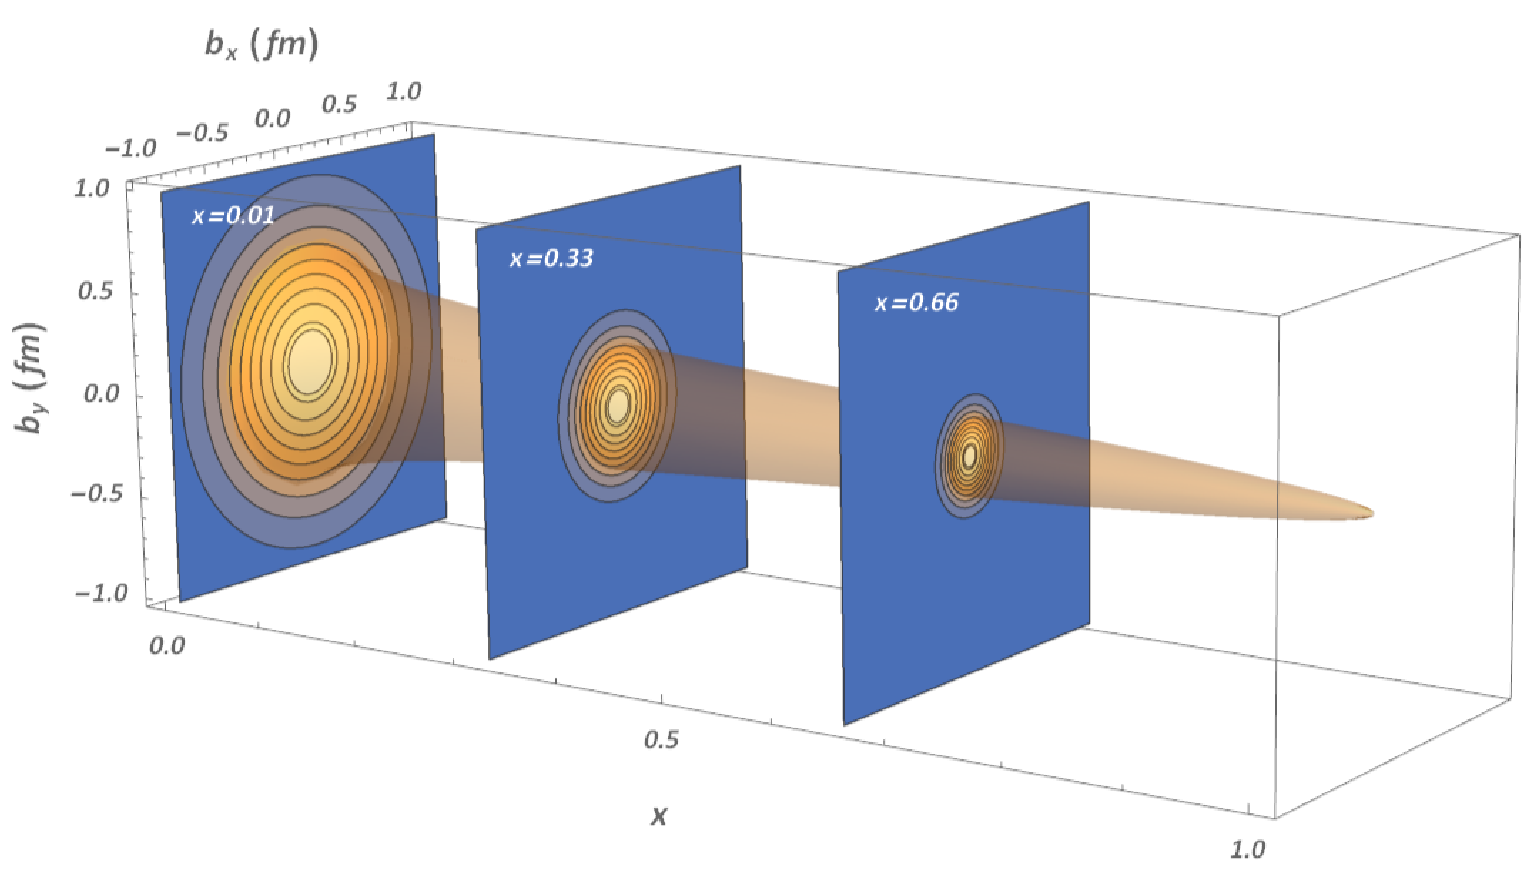
\includegraphics[width=0.4\linewidth]{figures/gpd_3D_imaging.png}
\end{frame}

\begin{frame}{Electron selection cuts}
    \begin{minipage}{0.49\linewidth}
        \begin{itemize}
            \item We select particles with pid = 11
            \item $Q^2 > 1 \mbox{ GeV}^2$
            \item $W^2 > 4 \mbox{ GeV}^2$
        \end{itemize}
    \end{minipage}
    \begin{minipage}{0.49\linewidth}
        \begin{itemize}
            \item $y < 0.85$
            \item $-26 \mbox{ cm} < \mbox{vz} < 17 \mbox{ cm}$
        \end{itemize}
    \end{minipage}
    

    \centering
    \vspace{0.2cm}

    \begin{minipage}{0.3\linewidth}
        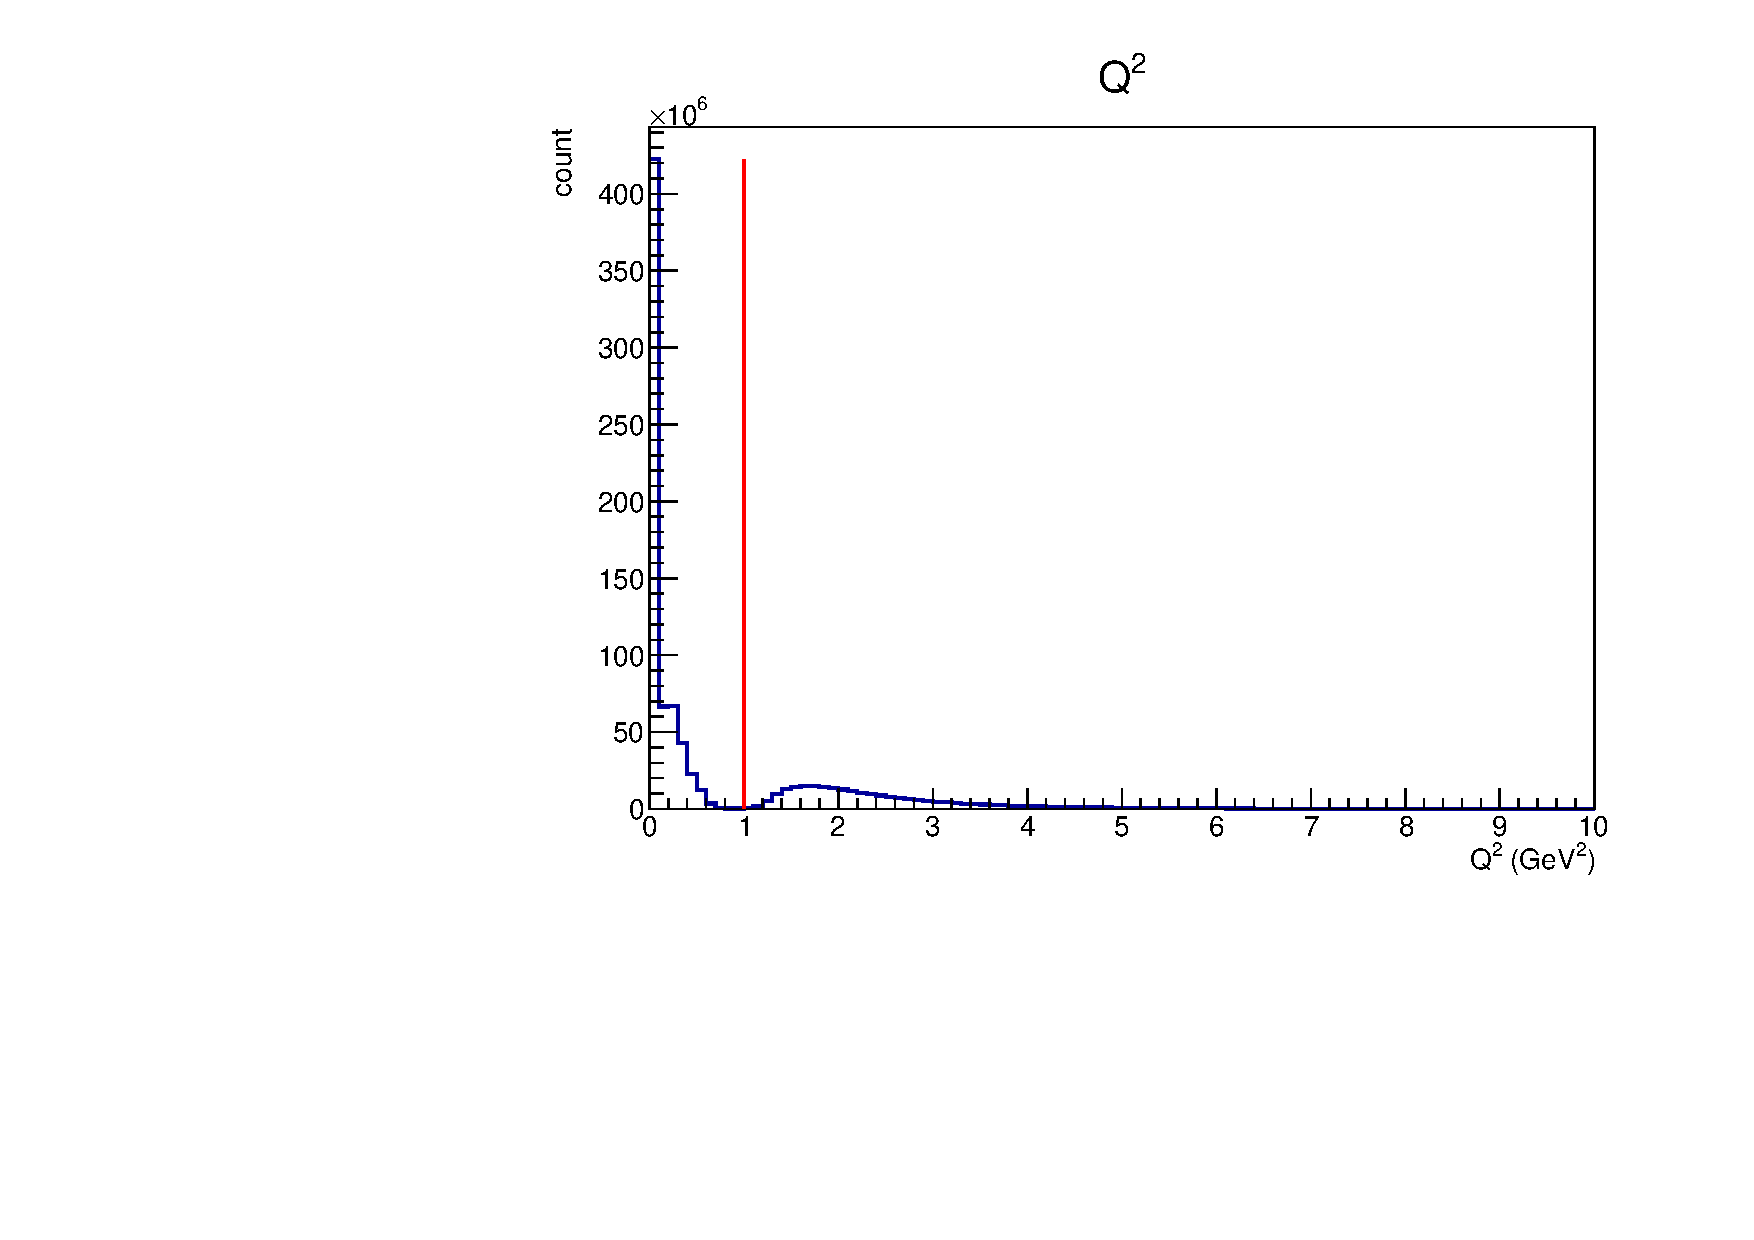
\includegraphics[width=\linewidth]{figures/q2_cut.pdf}
    \end{minipage}
    \begin{minipage}{0.3\linewidth}
        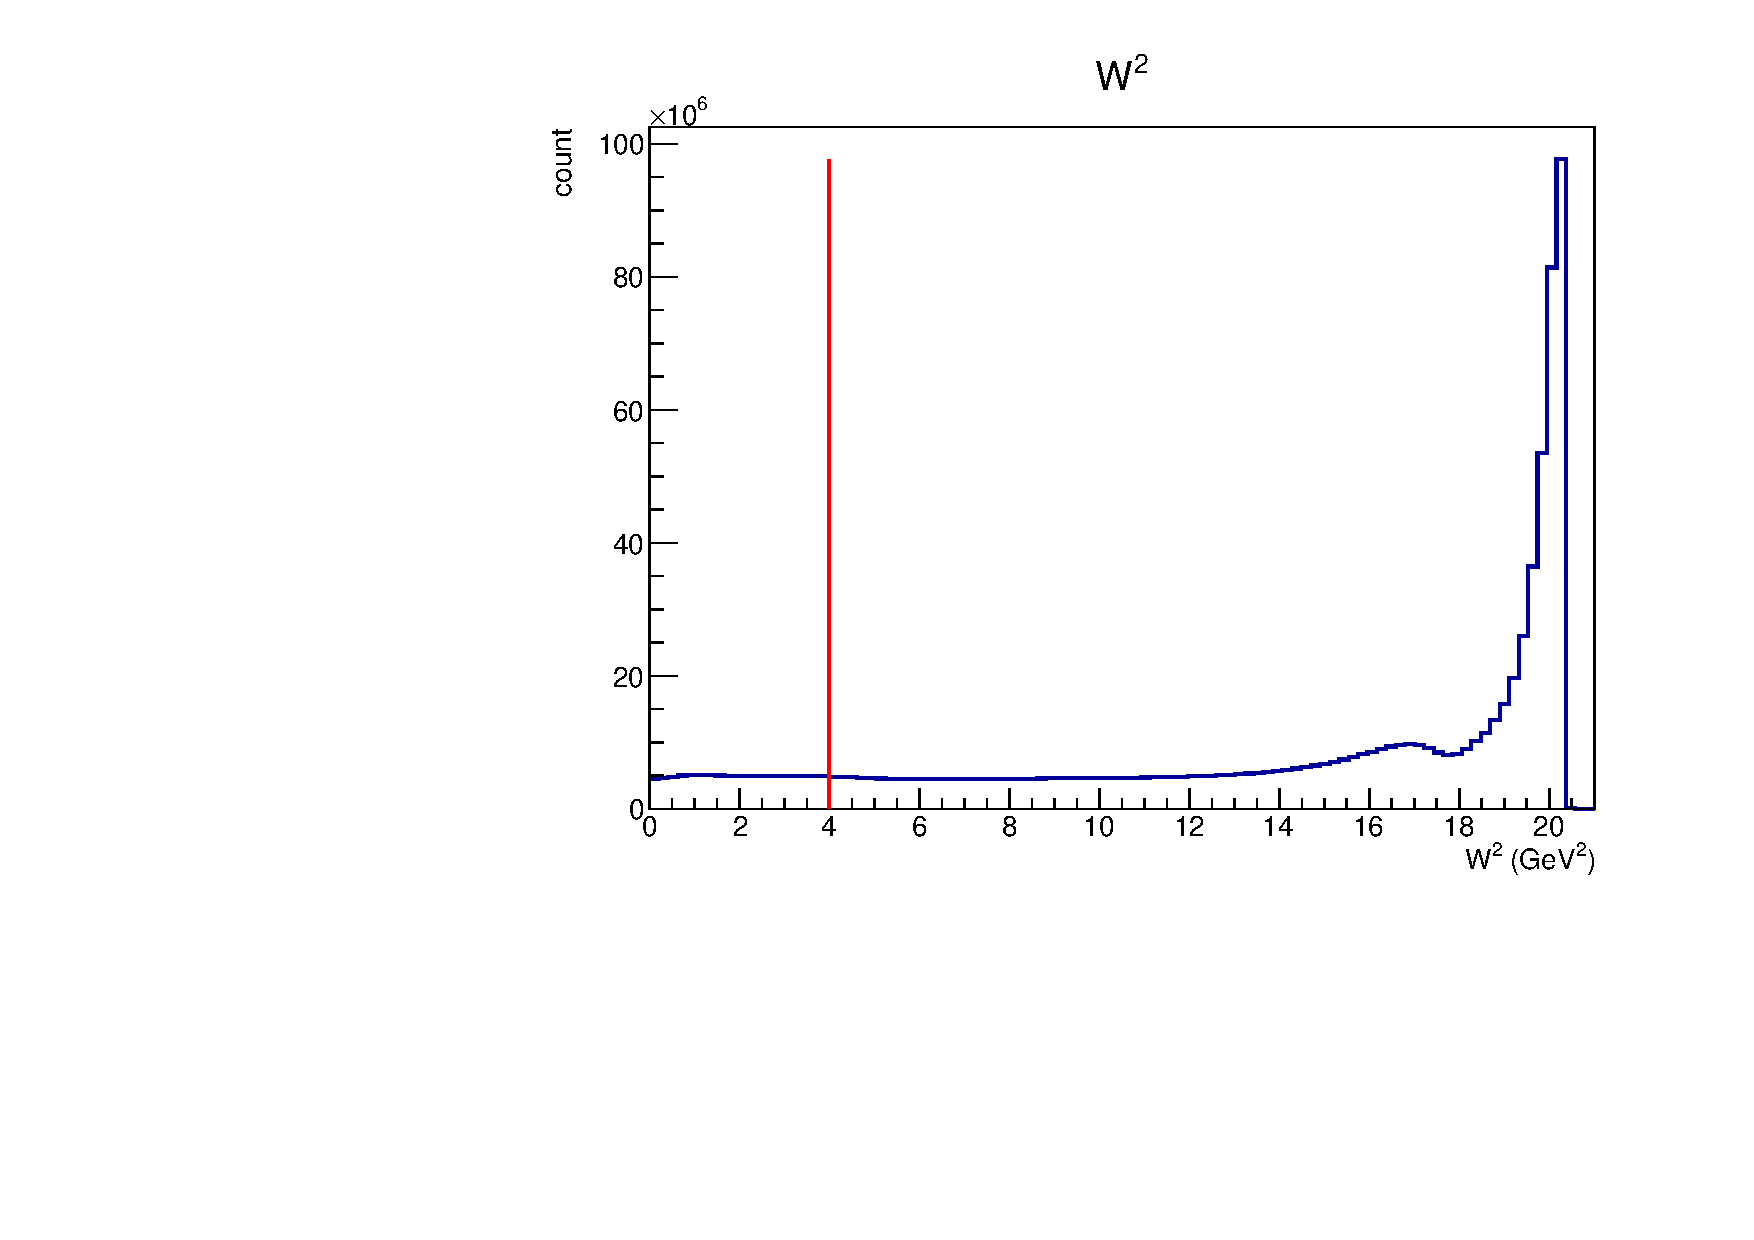
\includegraphics[width=\linewidth]{figures/w2_cut.pdf}
    \end{minipage}
    \begin{minipage}{0.3\linewidth}
        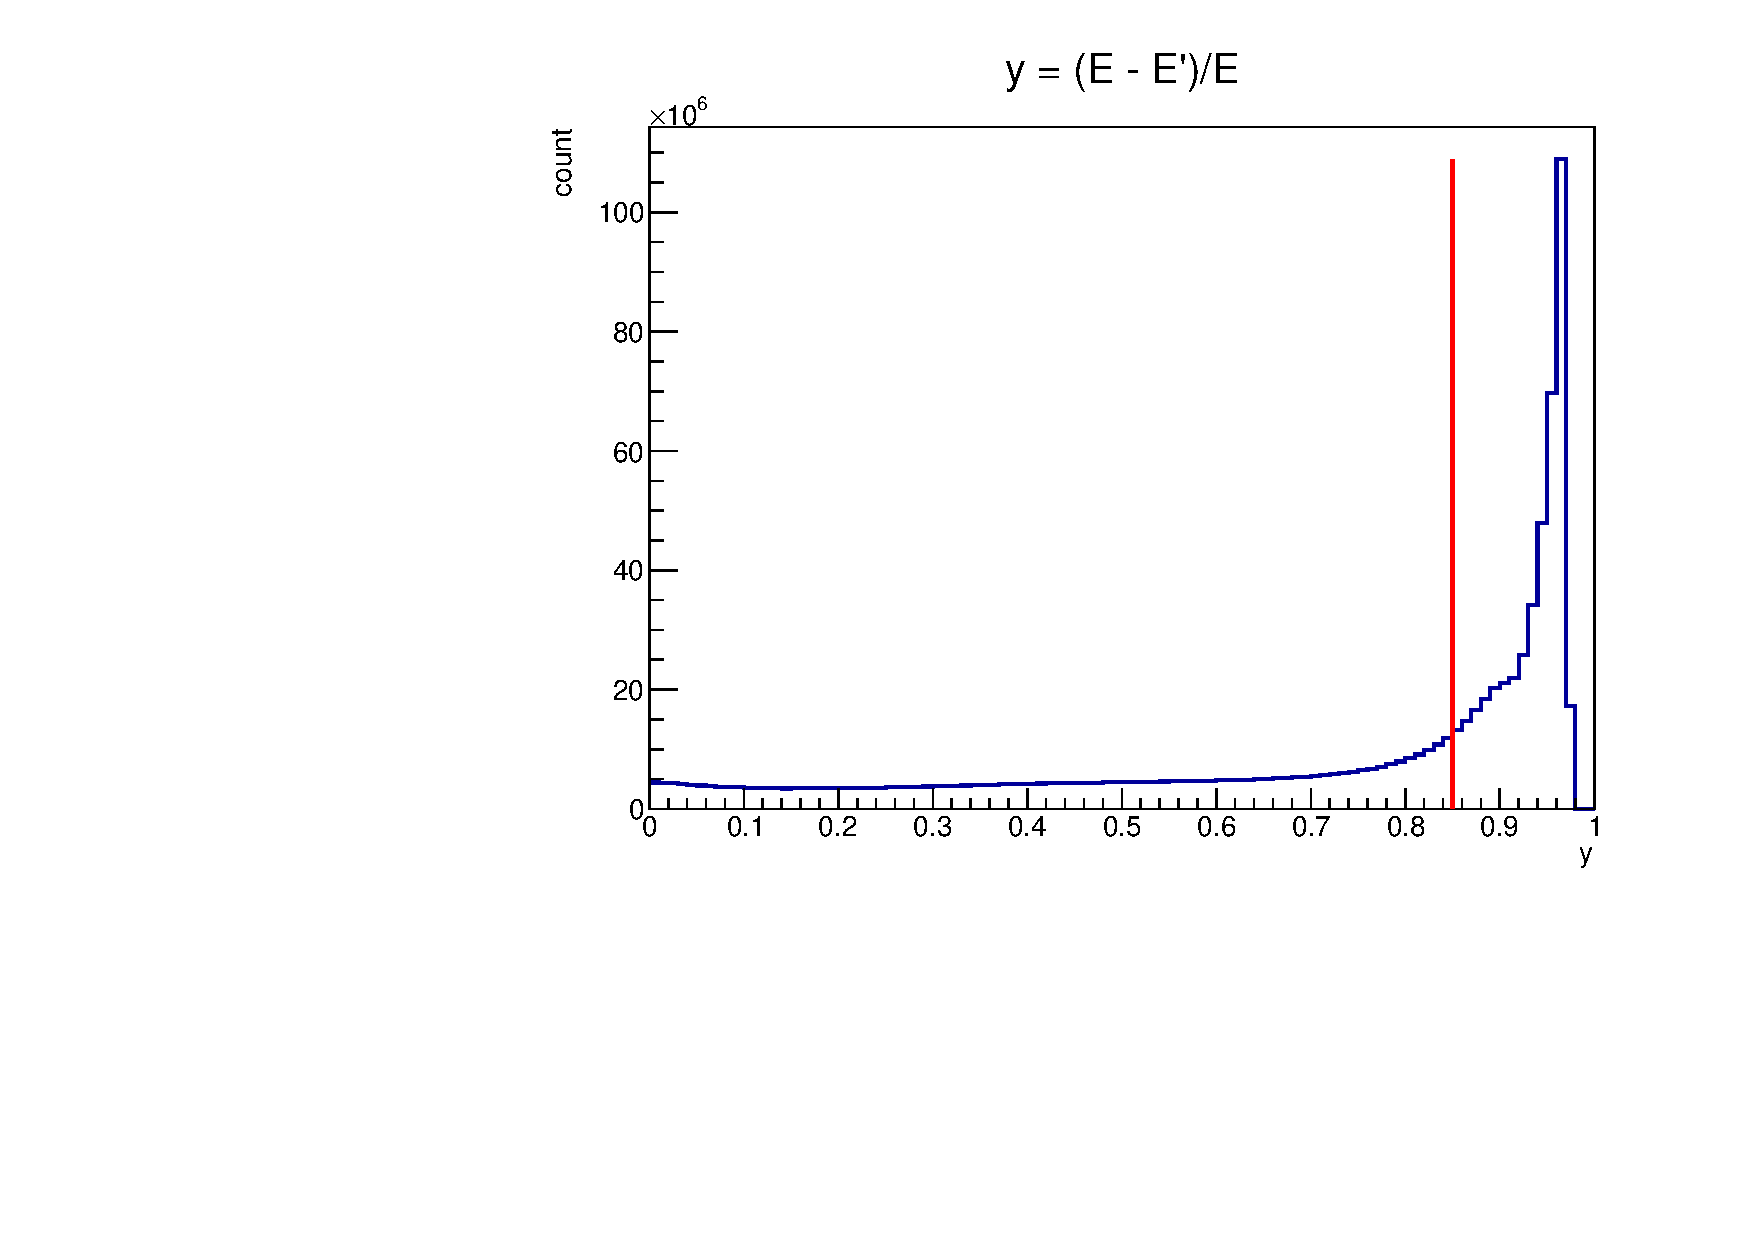
\includegraphics[width=\linewidth]{figures/y_cut.pdf}
    \end{minipage}
    \begin{minipage}{0.3\linewidth}
        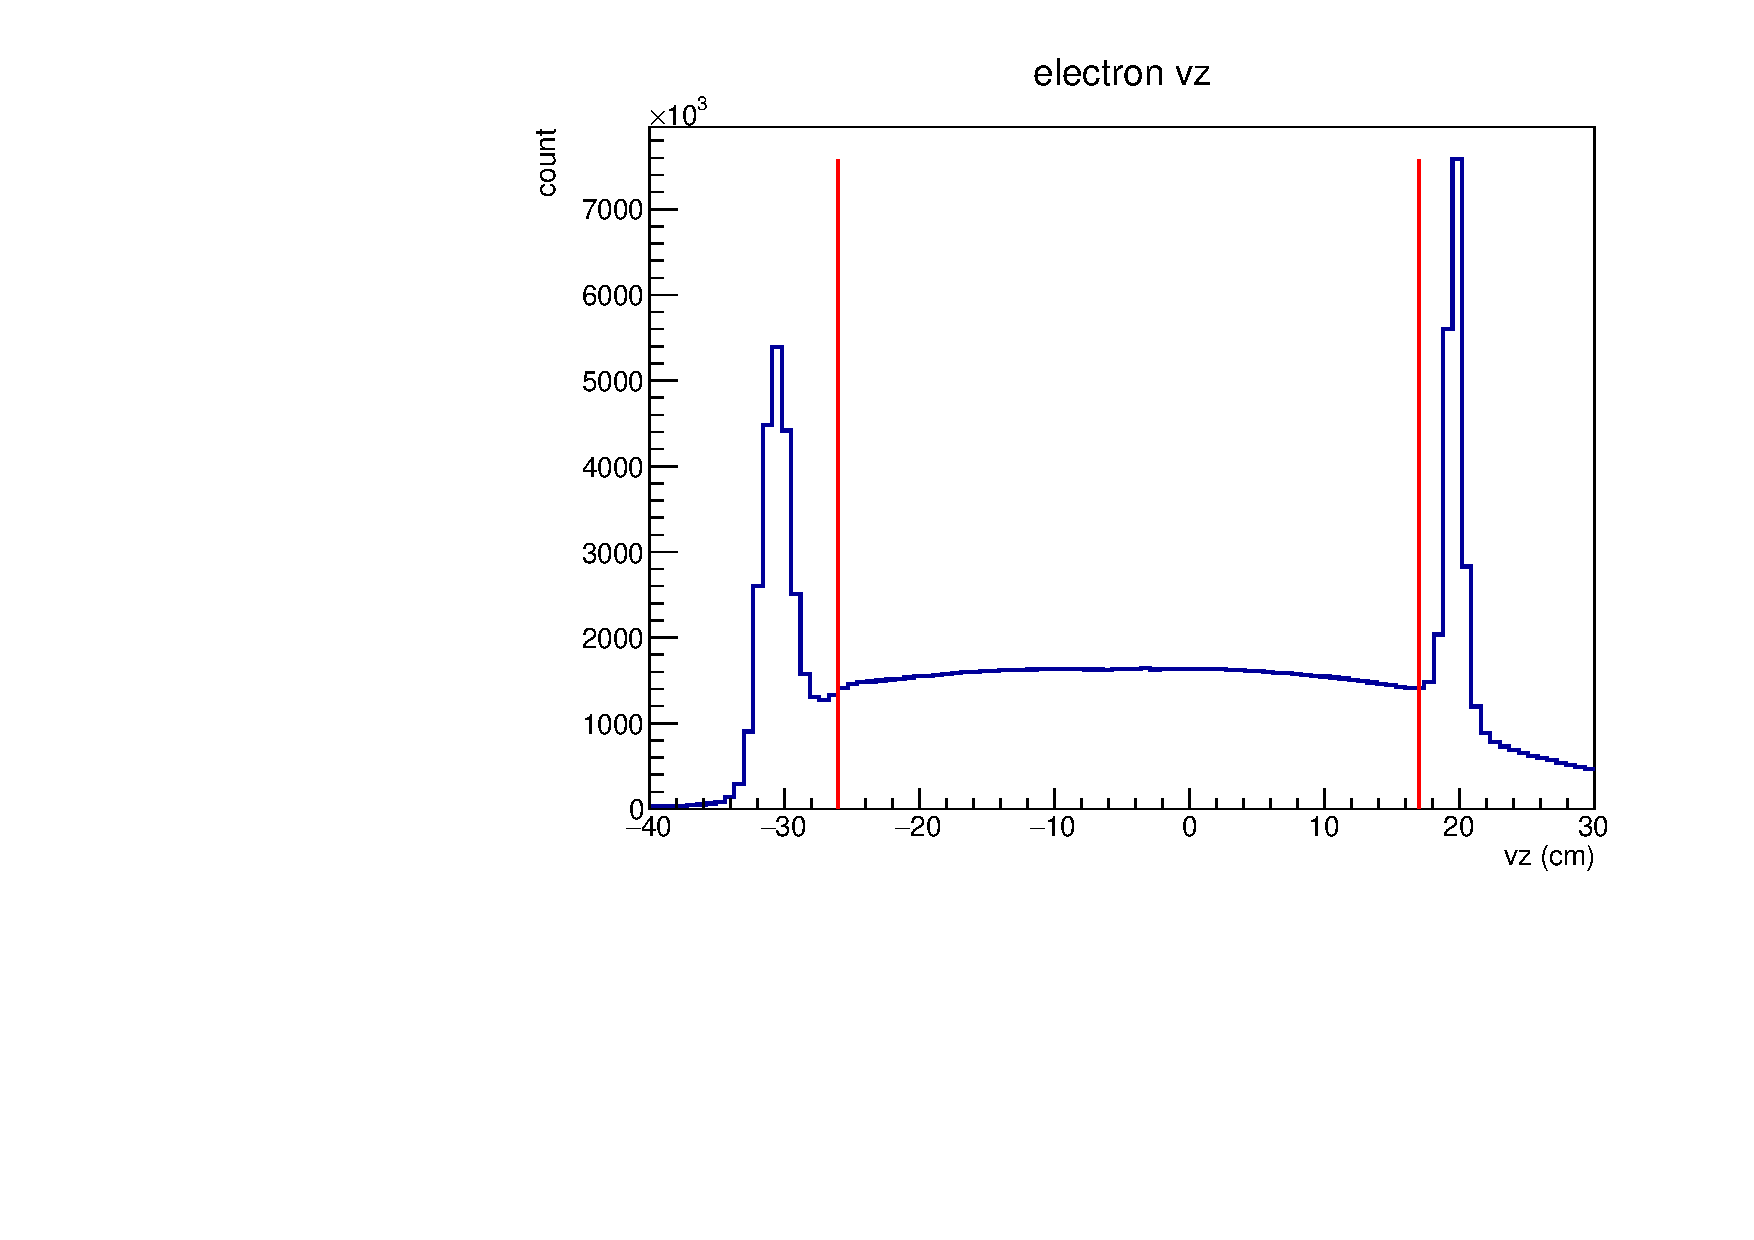
\includegraphics[width=\linewidth]{figures/vz_cut.pdf}
    \end{minipage}

\end{frame}

\begin{frame}{Electron distributions after cuts}

    \centering
    \vspace{0.2cm}
    \begin{minipage}{0.3\linewidth}
        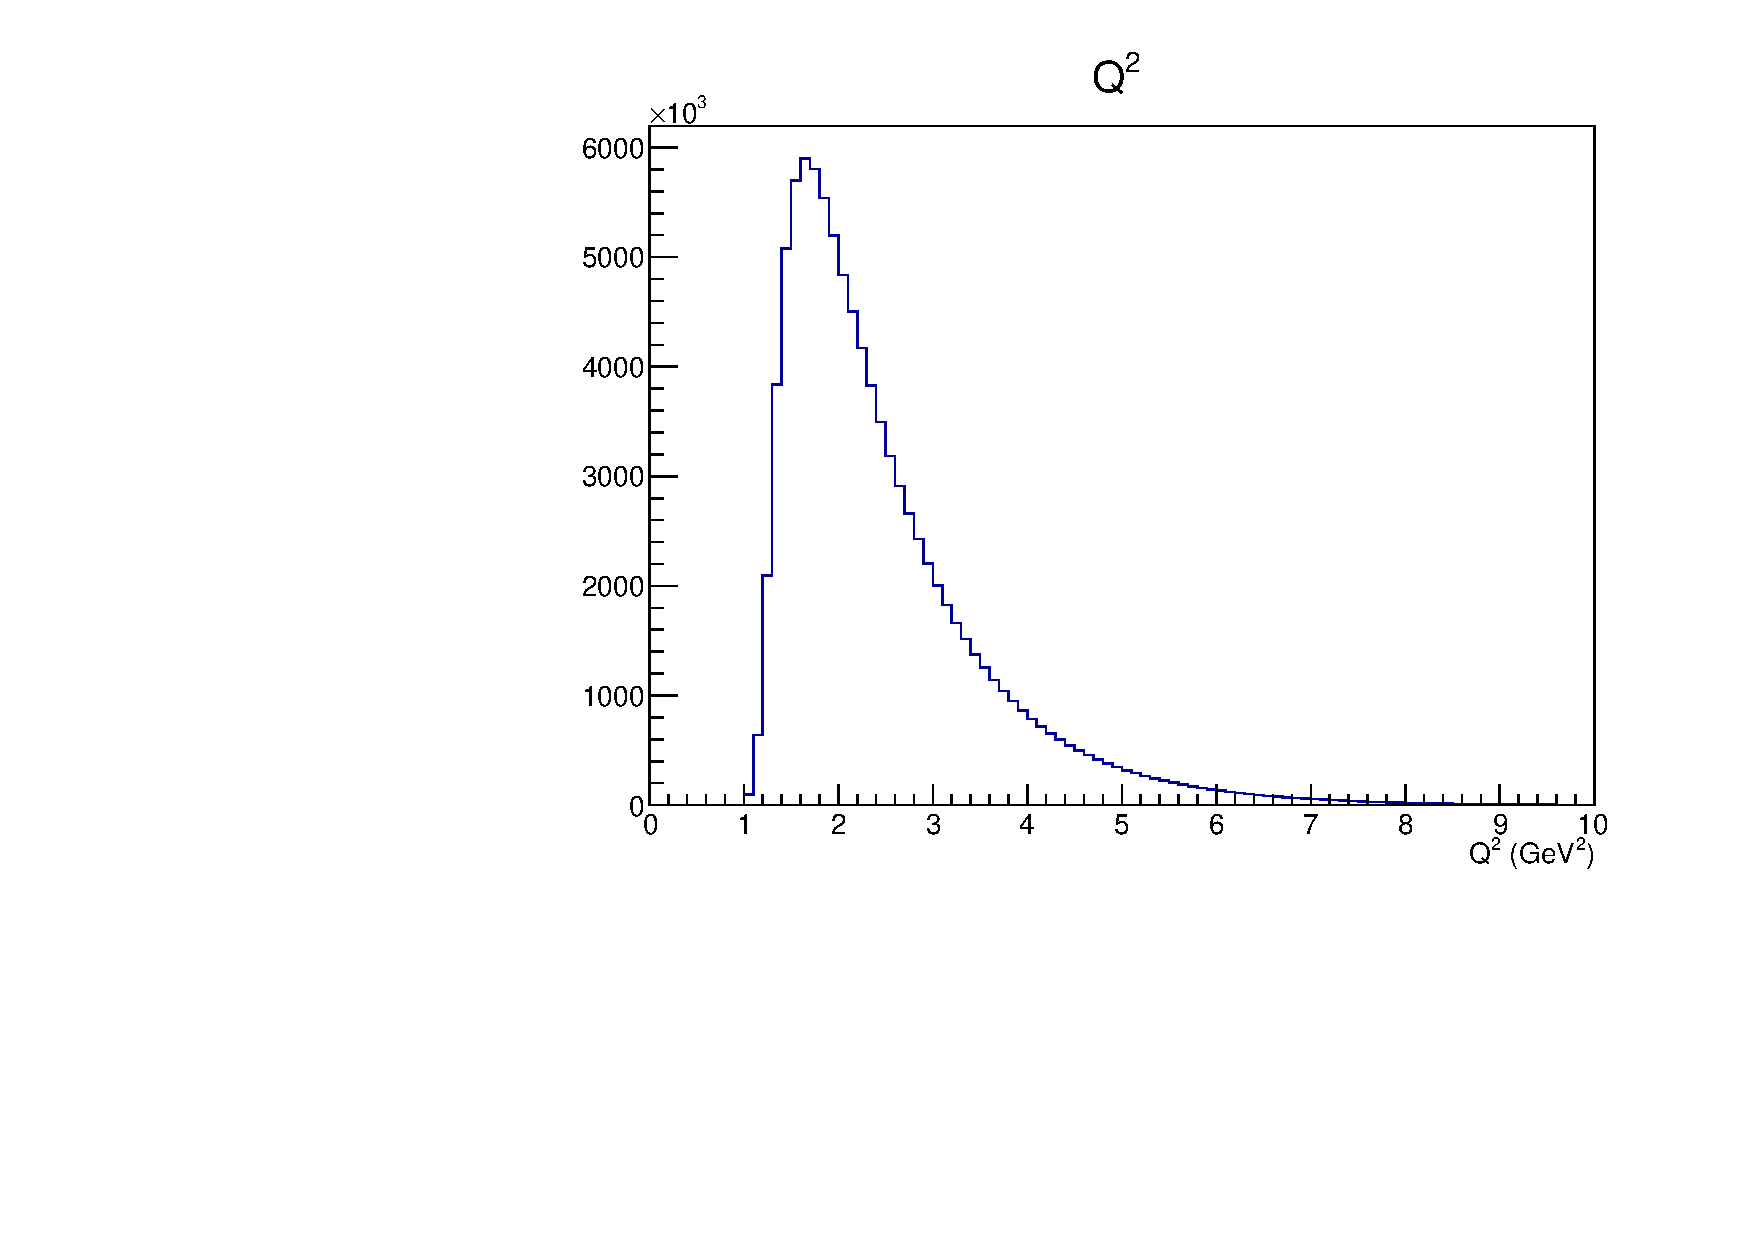
\includegraphics[width=\linewidth]{figures/Q2_q2w2yvz_cut.pdf}
    \end{minipage}
    \begin{minipage}{0.3\linewidth}
        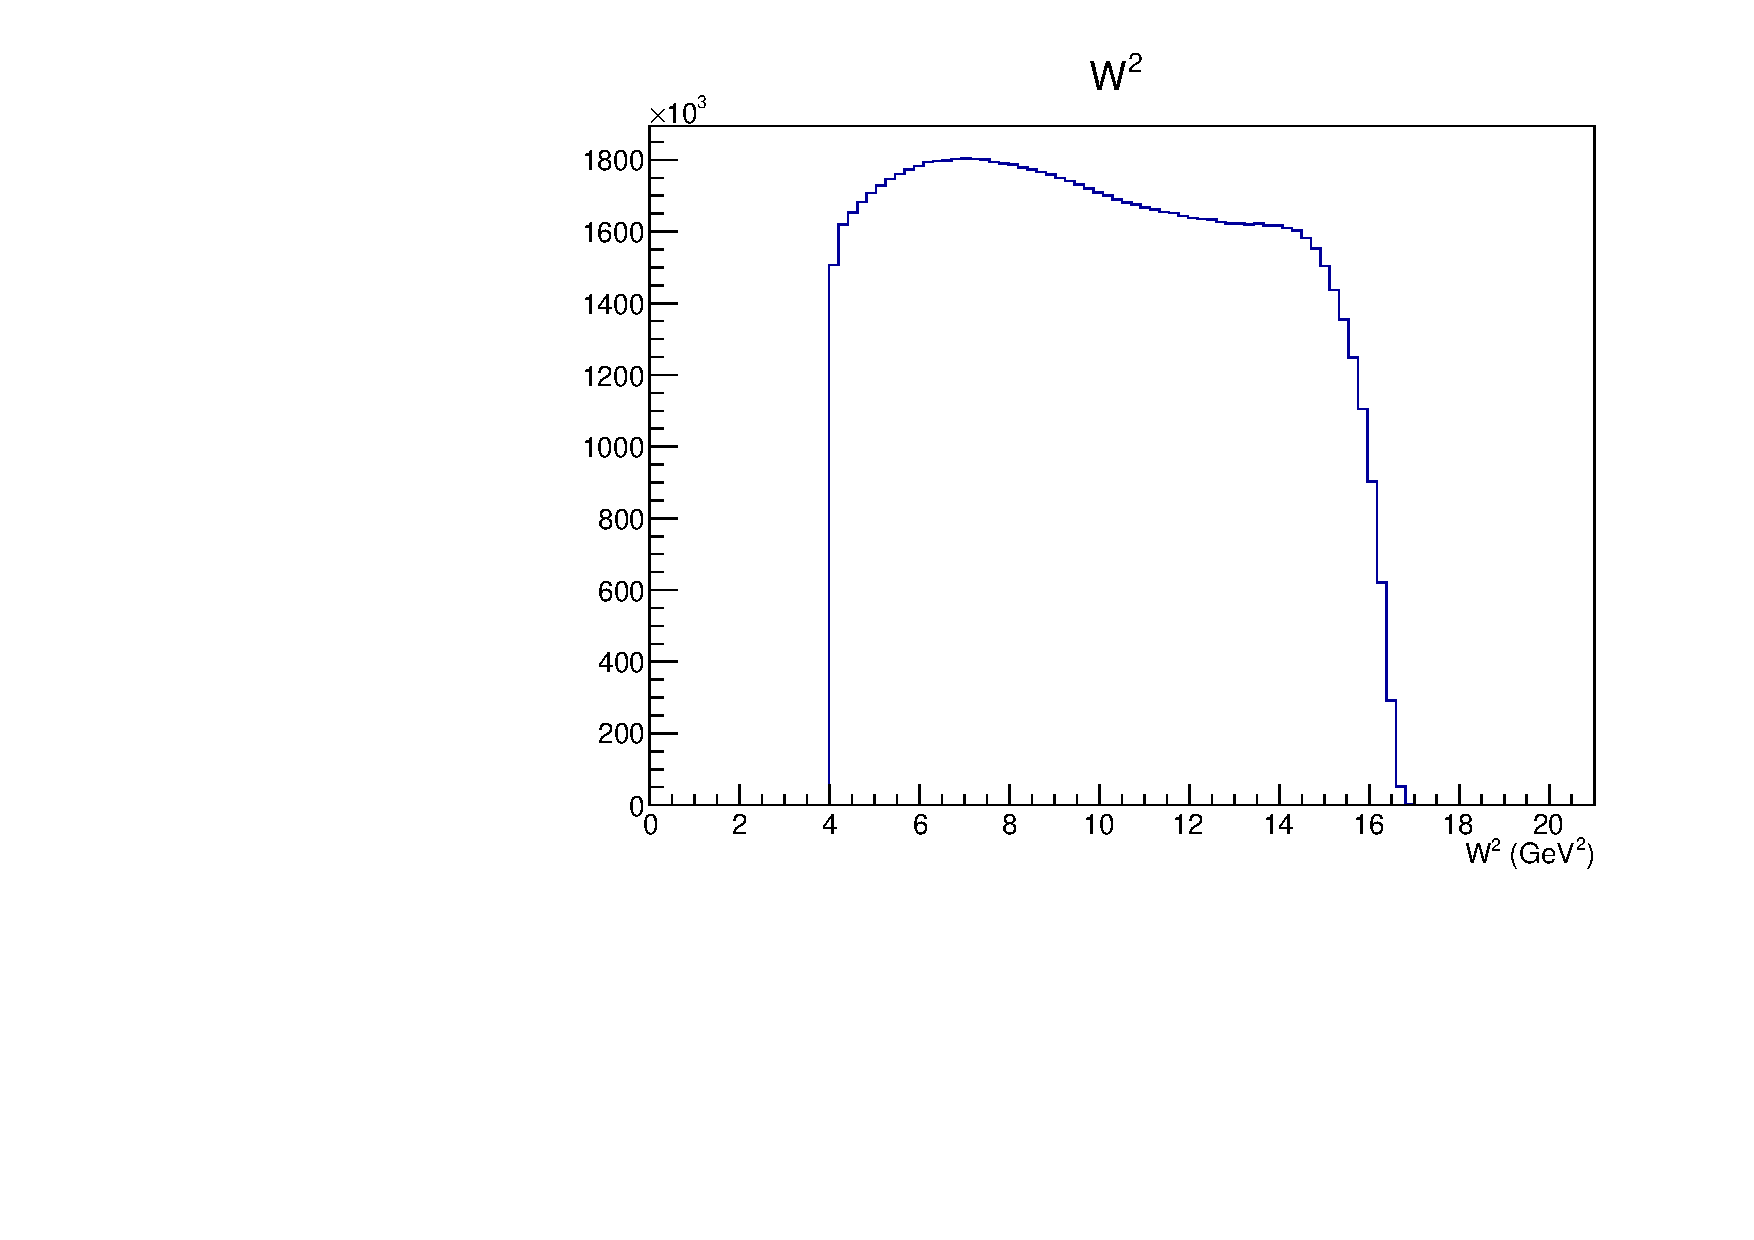
\includegraphics[width=\linewidth]{figures/W2_q2w2yvz_cut.pdf}
    \end{minipage}
    \begin{minipage}{0.3\linewidth}
        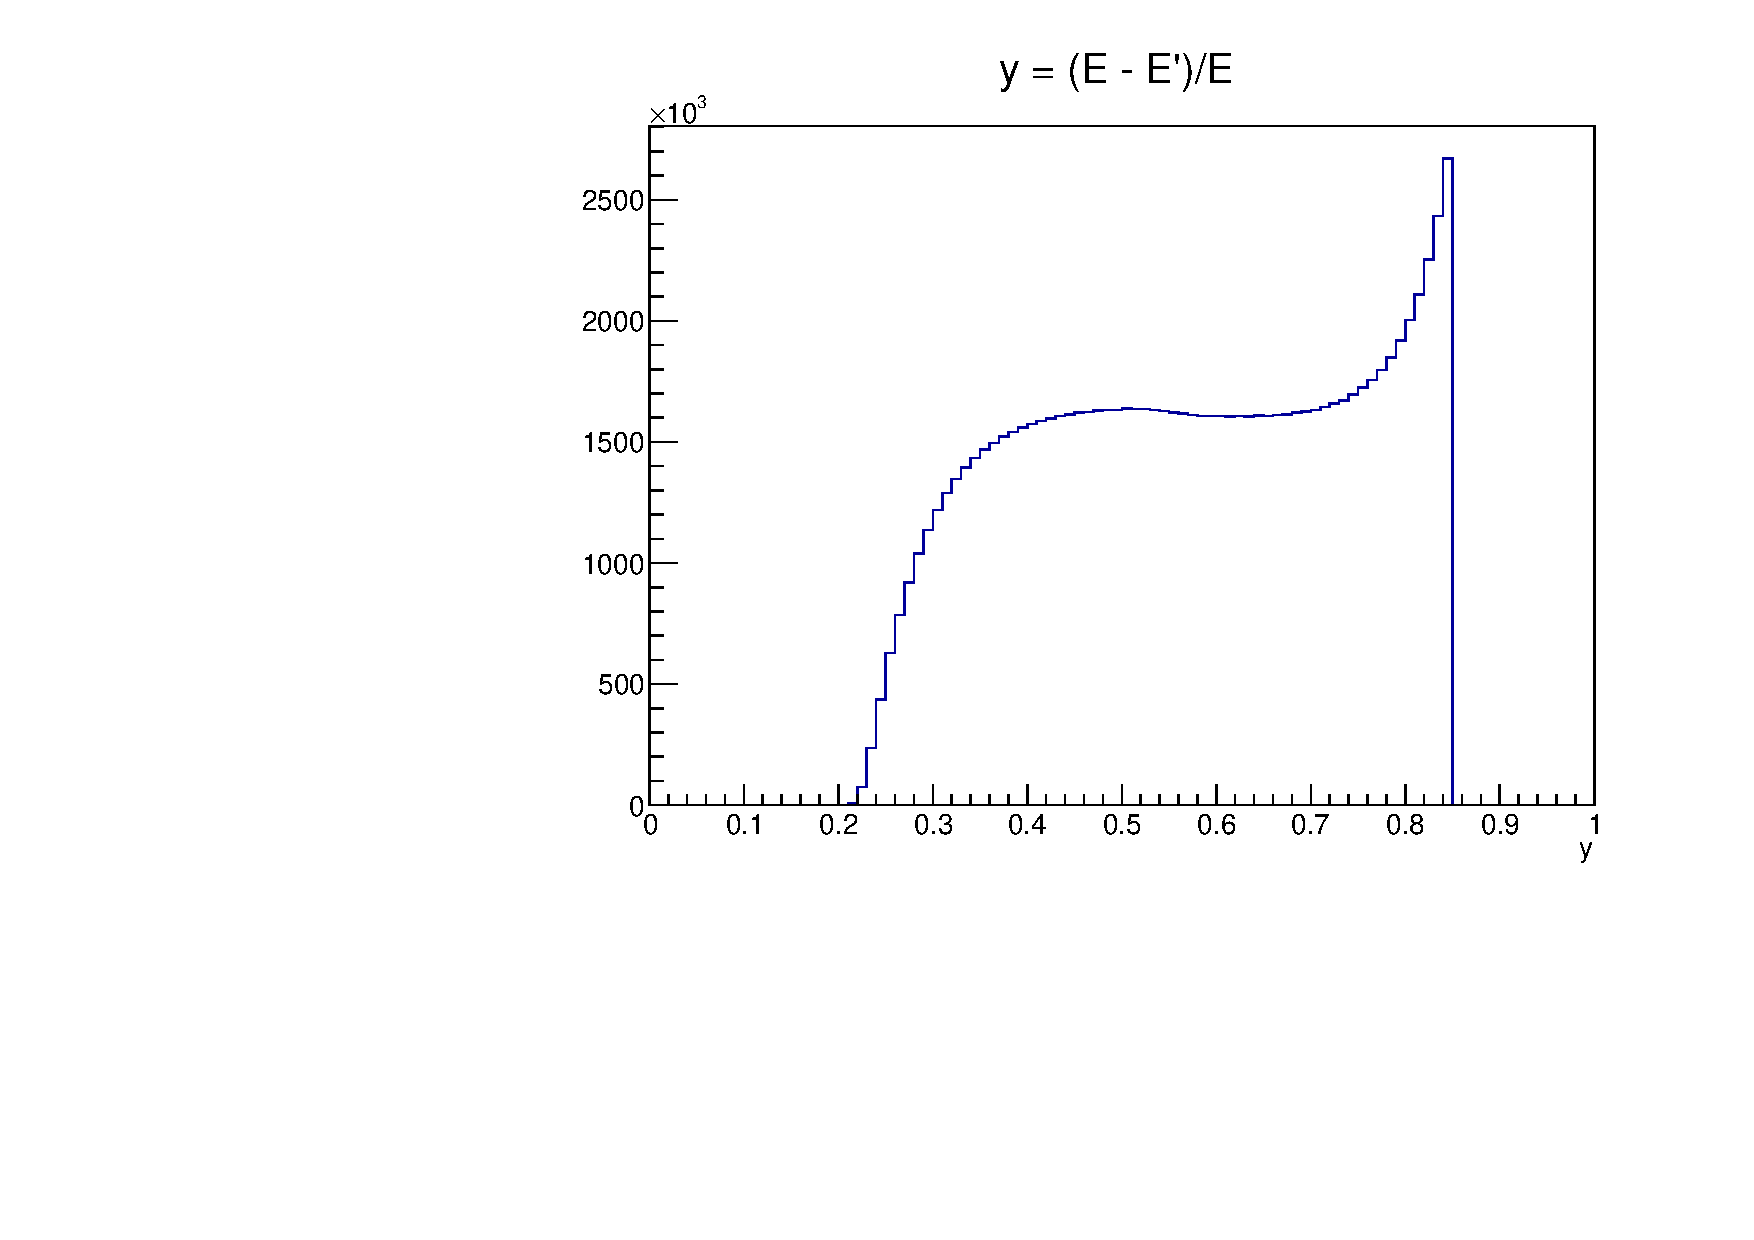
\includegraphics[width=\linewidth]{figures/y_q2w2yvz_cut.pdf}
    \end{minipage}
    \begin{minipage}{0.3\linewidth}
        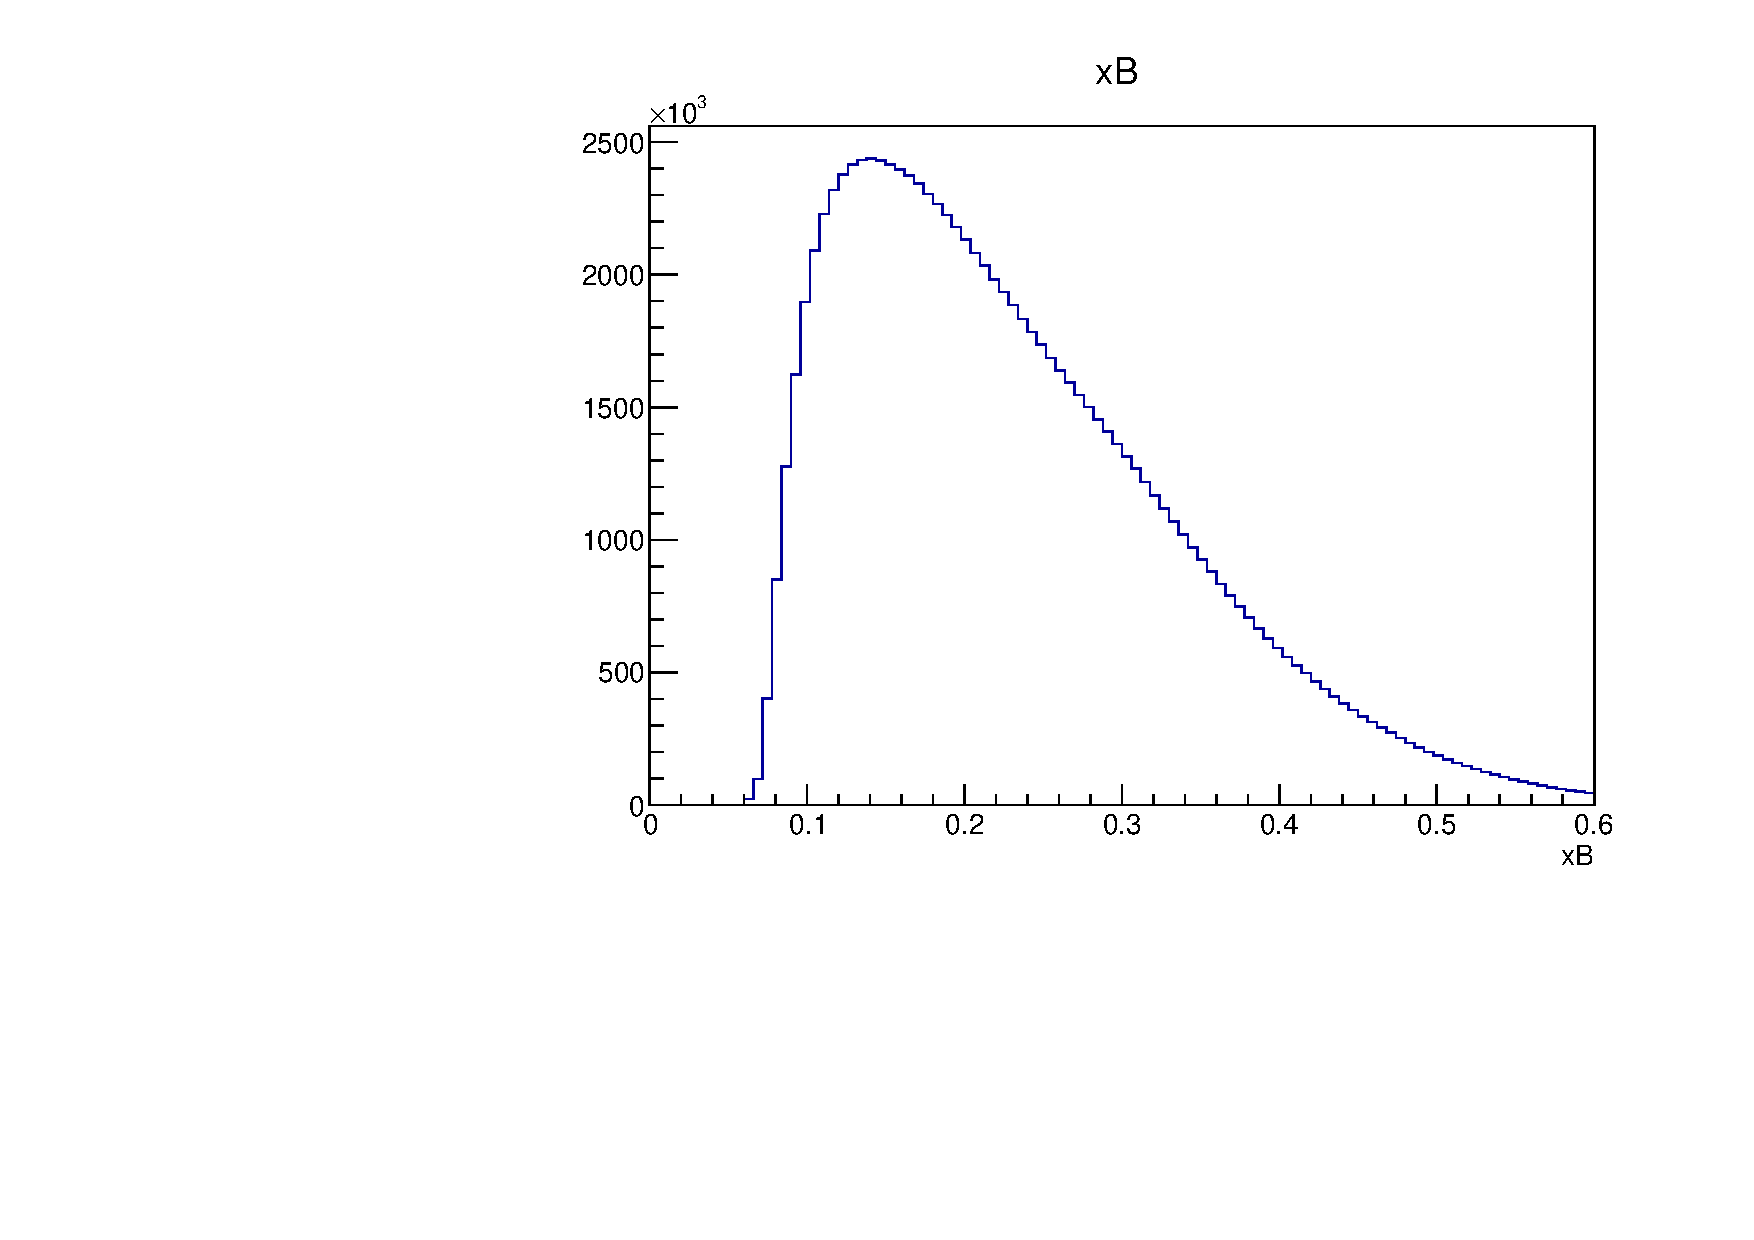
\includegraphics[width=\linewidth]{figures/xB_q2w2yvz_cut.pdf}
    \end{minipage}
    \begin{minipage}{0.3\linewidth}
        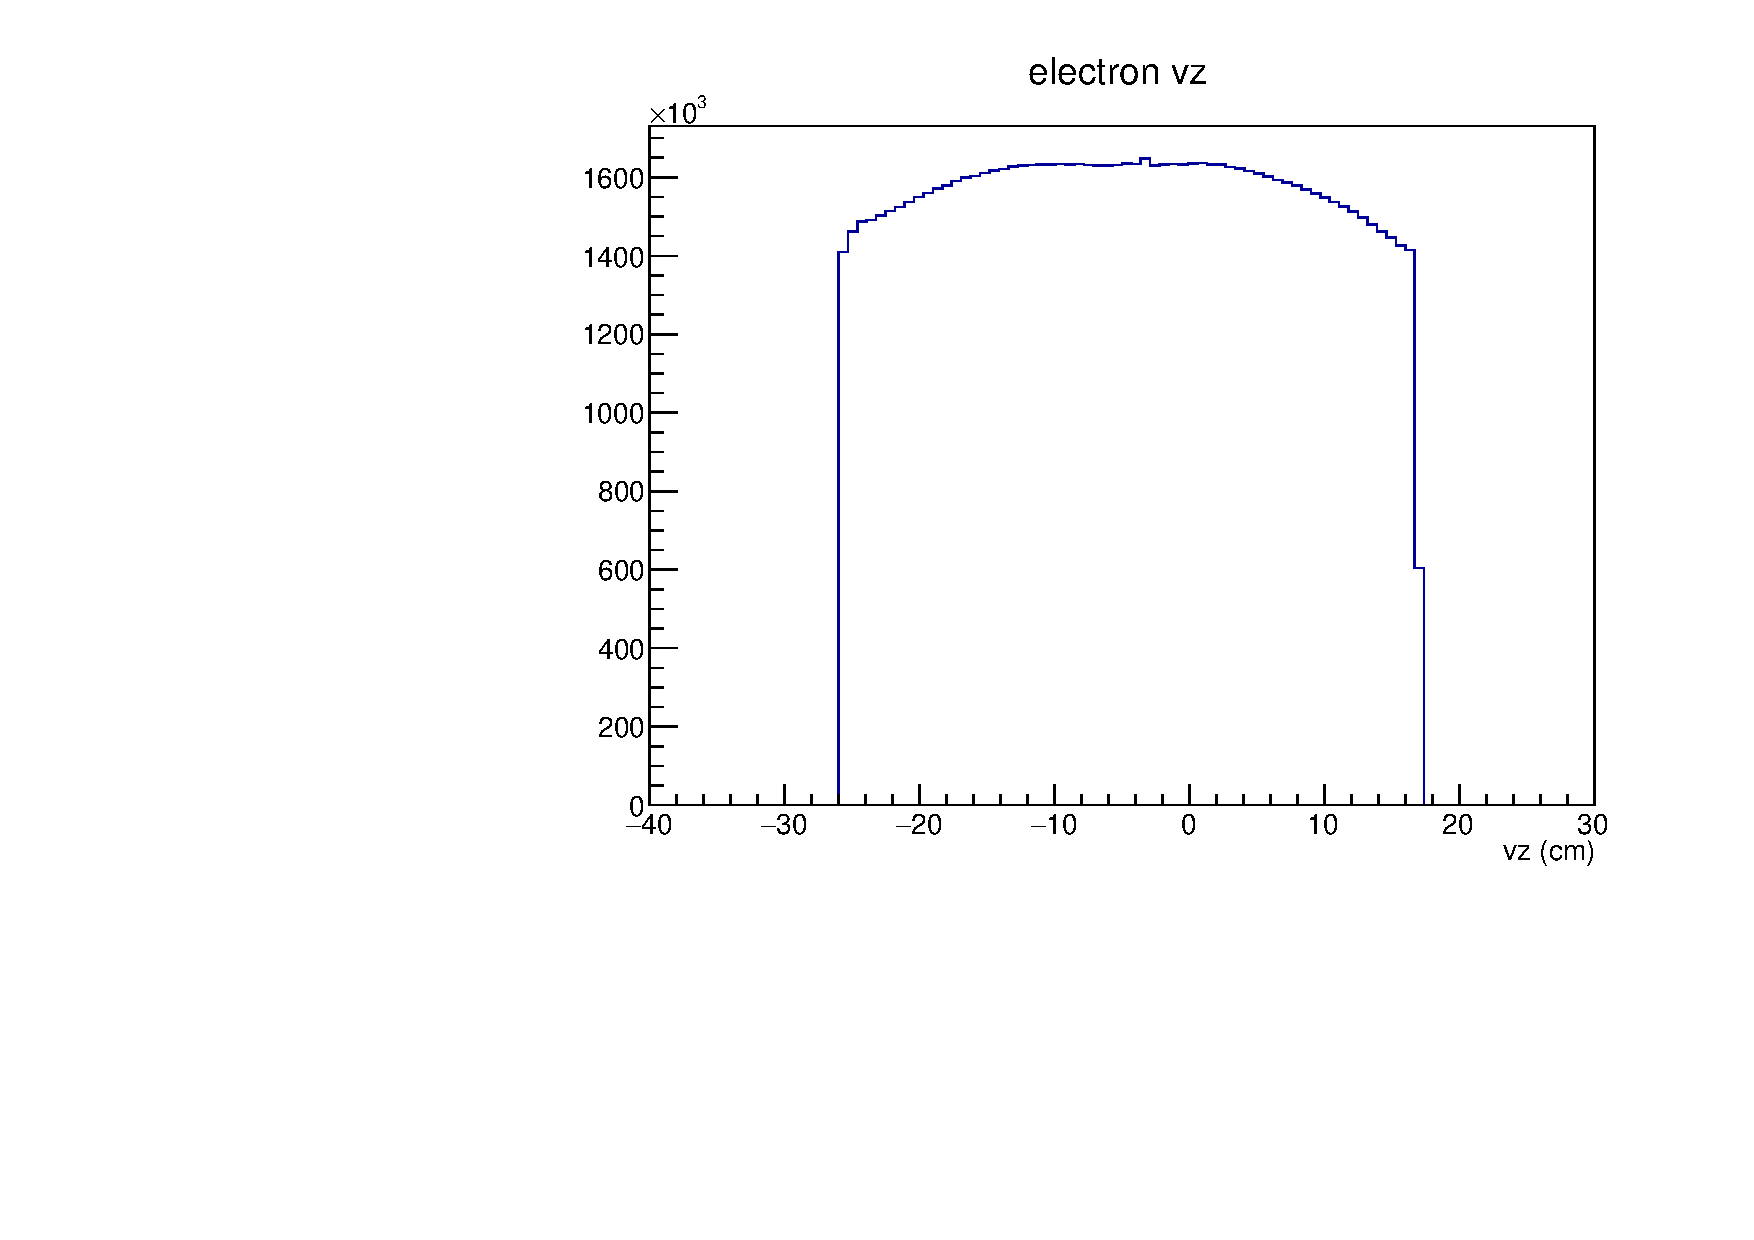
\includegraphics[width=\linewidth]{figures/electron_vz_q2w2yvz_cut.pdf}
    \end{minipage}
    \begin{minipage}{0.3\linewidth}
        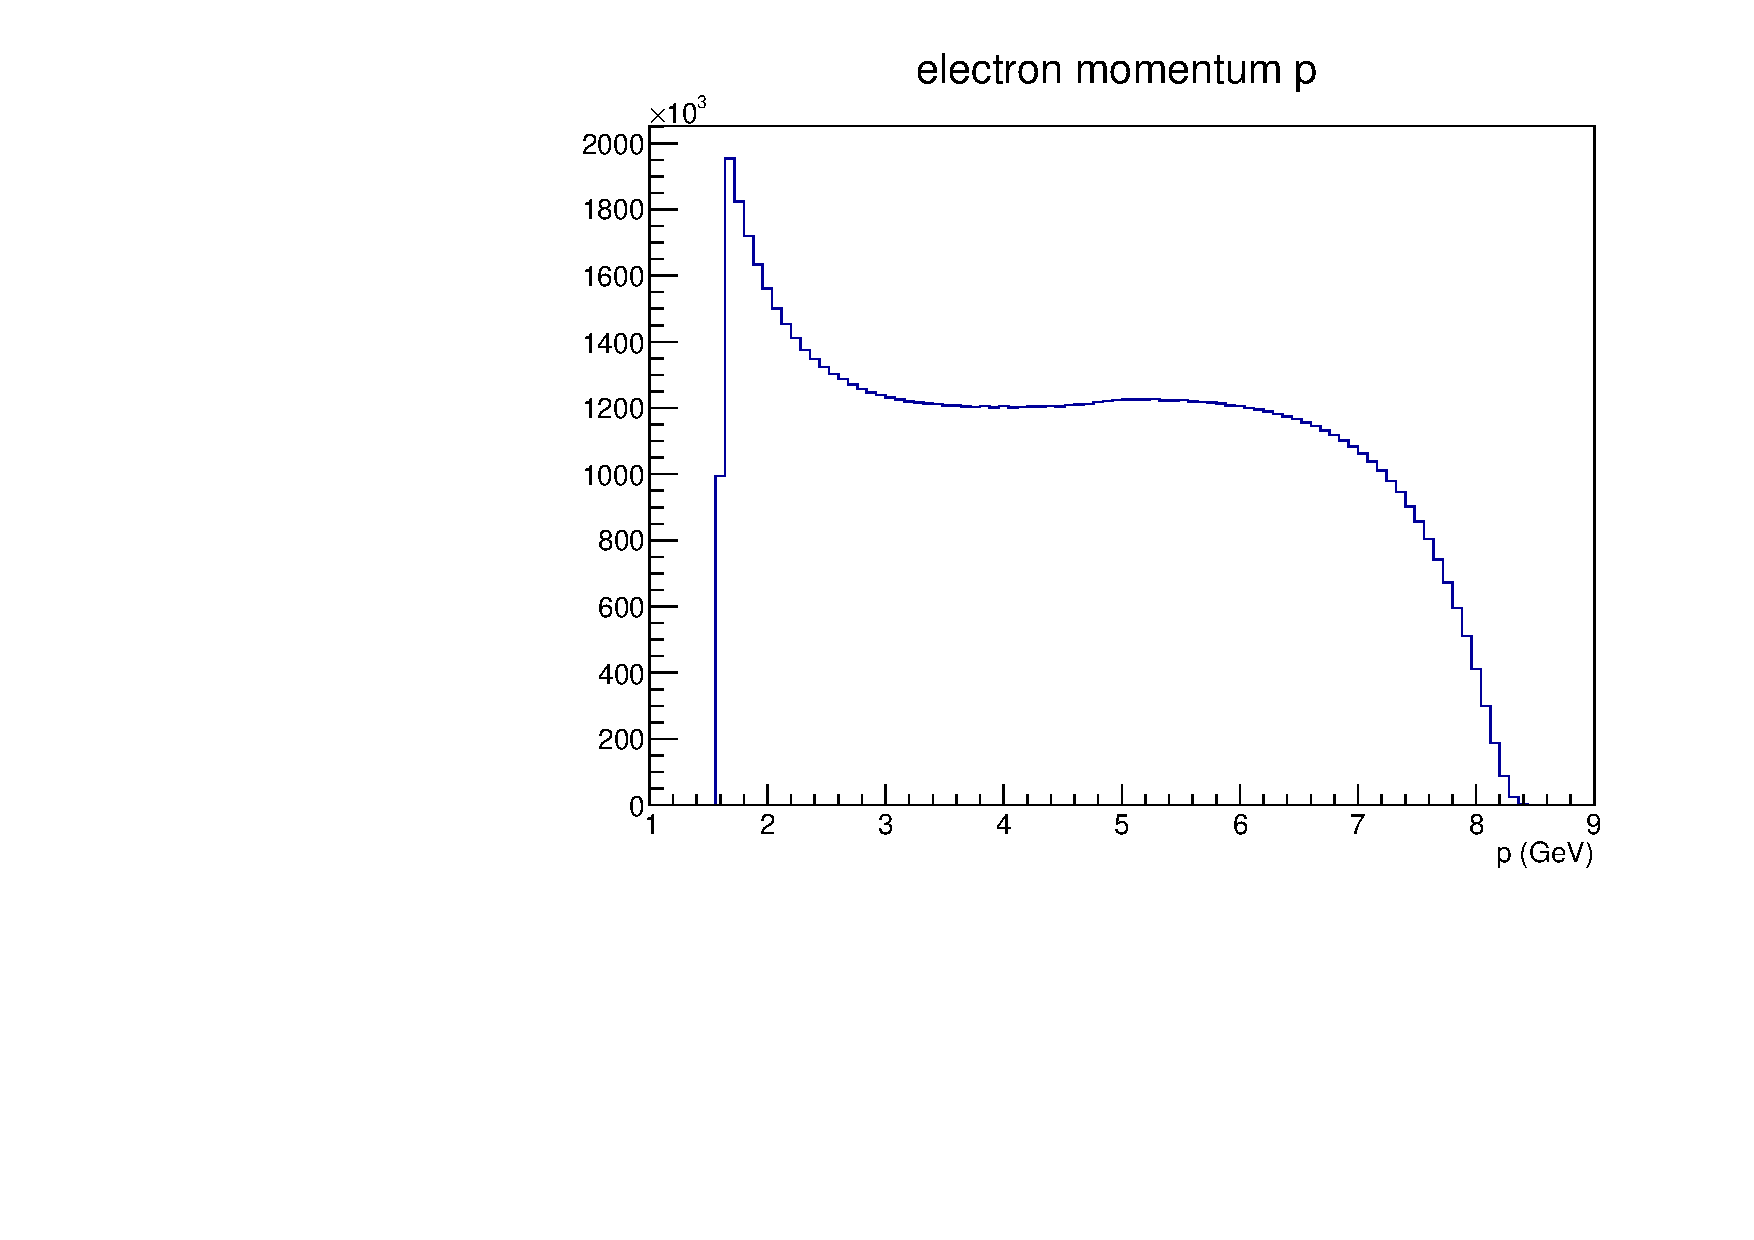
\includegraphics[width=\linewidth]{figures/electron_p_q2w2yvz_cut.pdf}
    \end{minipage}
    \begin{minipage}{0.3\linewidth}
        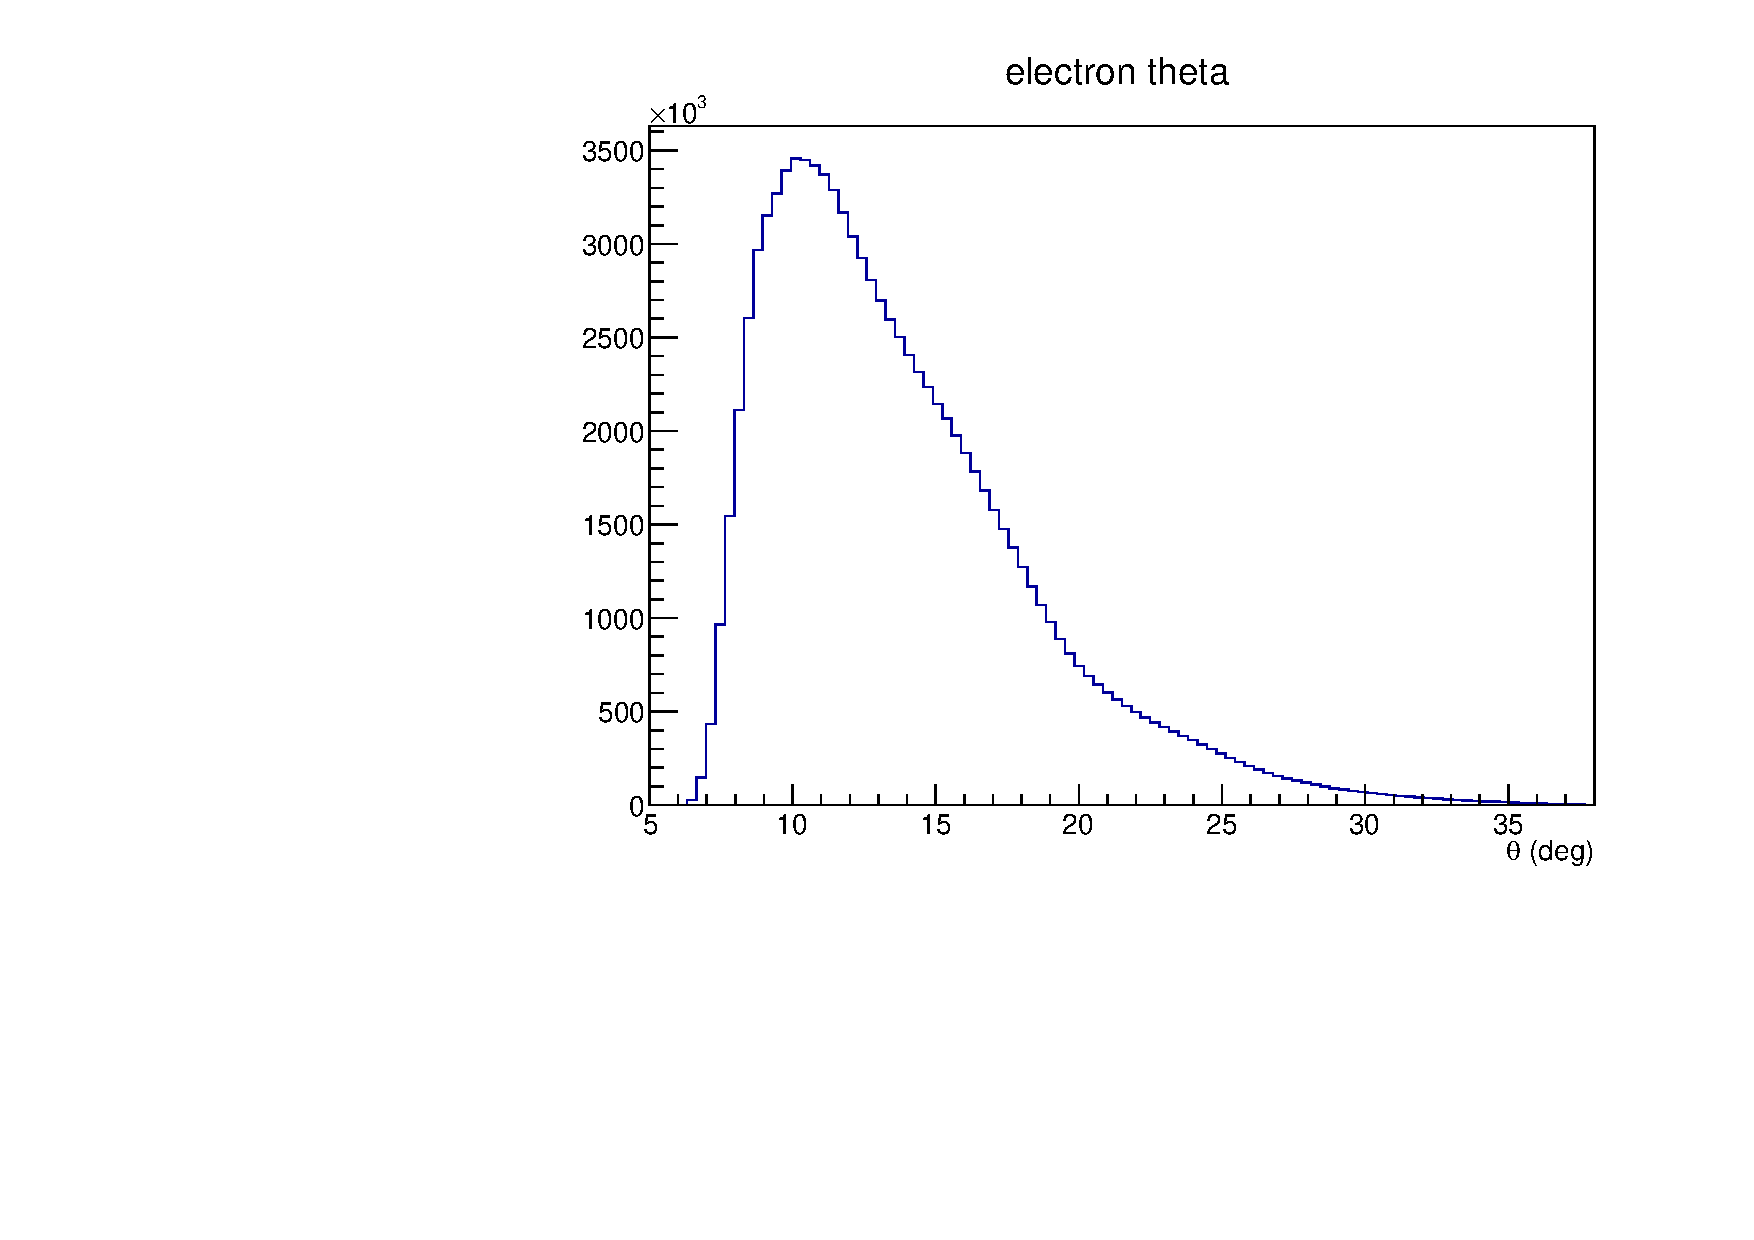
\includegraphics[width=\linewidth]{figures/electron_theta_q2w2yvz_cut.pdf}
    \end{minipage}
    \begin{minipage}{0.3\linewidth}
        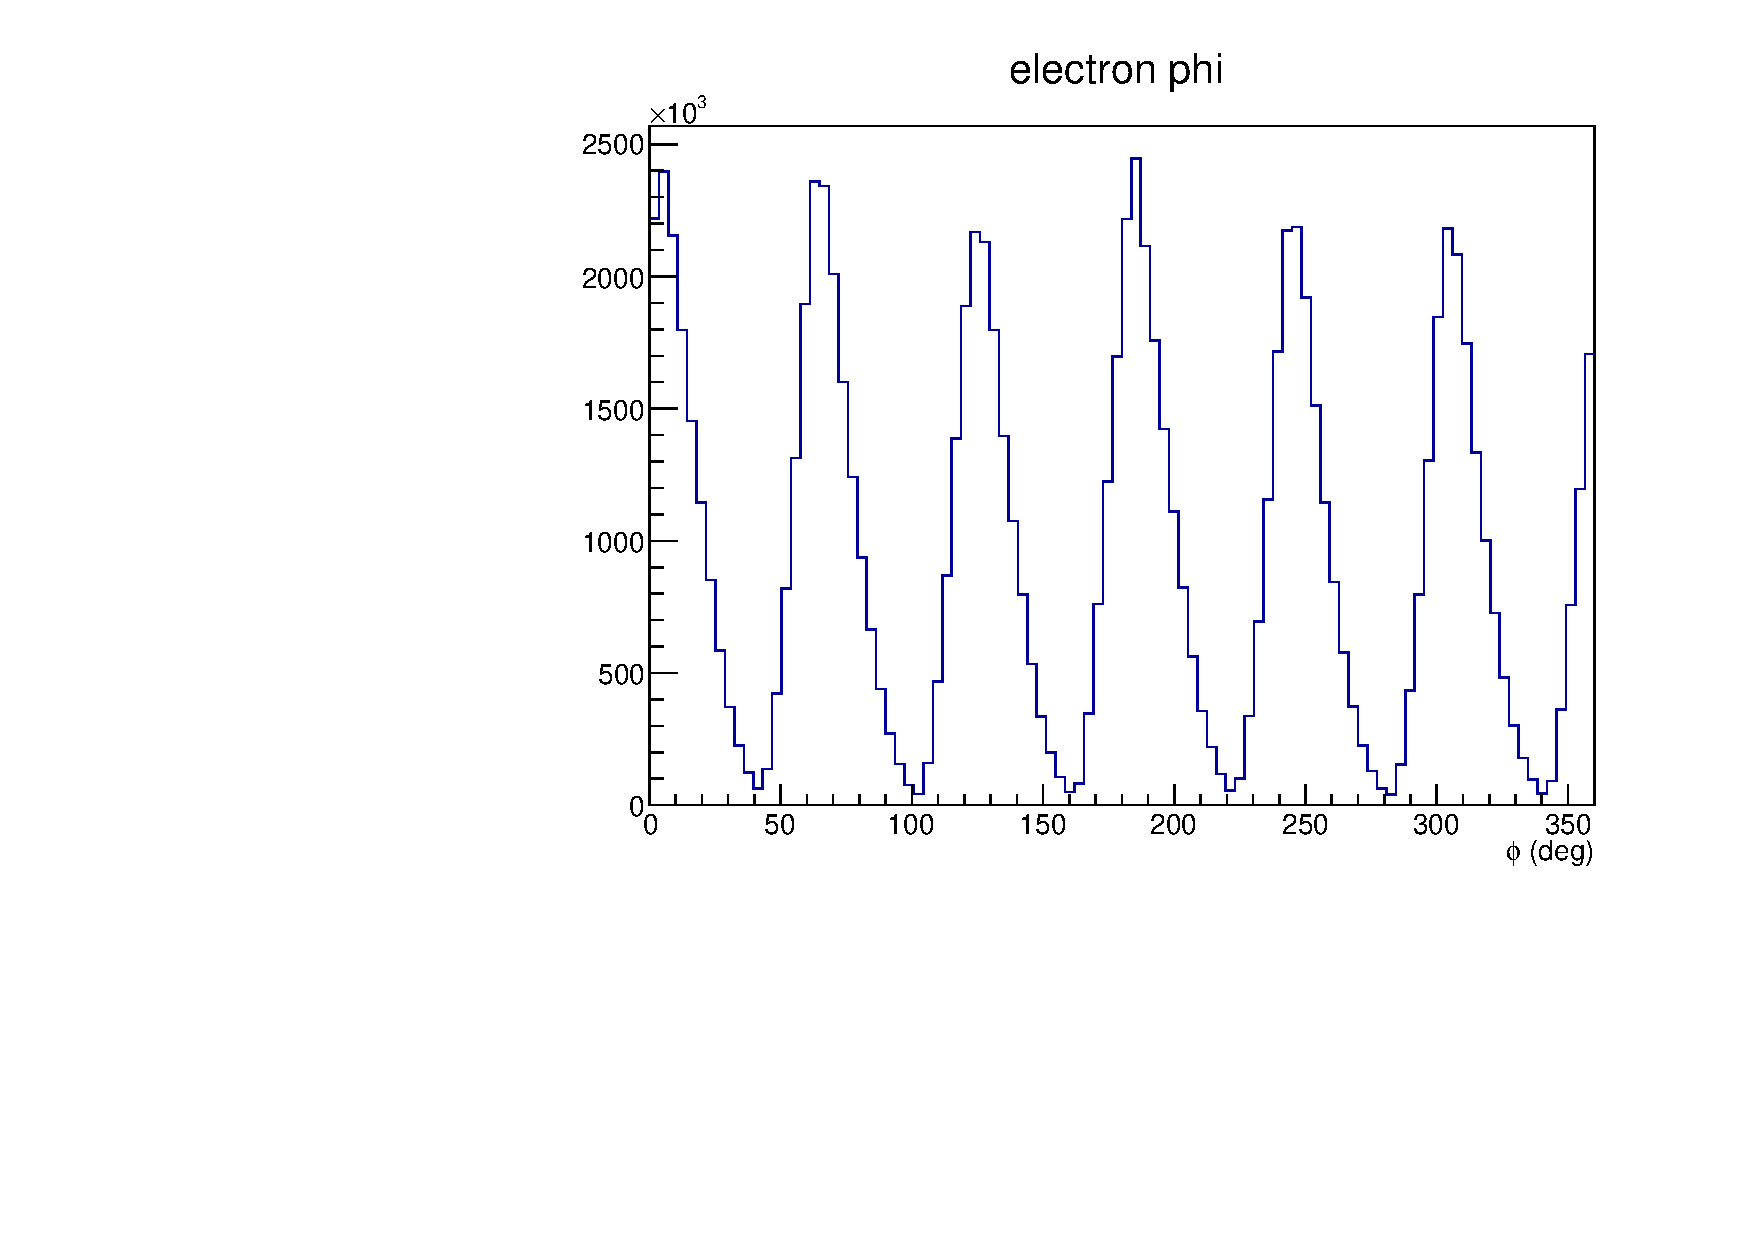
\includegraphics[width=\linewidth]{figures/electron_phi_q2w2yvz_cut.pdf}
    \end{minipage}
    

\end{frame}

\begin{frame}{Photon selection cuts and distributions}
    \begin{itemize}
        \item We require the detection of 1 electron
        \item We select particle with pid = 22
        \item We select high energy photons : $p_{\gamma} > 1.5 \mbox{ GeV}$
    \end{itemize}

    \centering
    \vspace{0.2cm}
    
    \begin{minipage}{0.3\linewidth}
        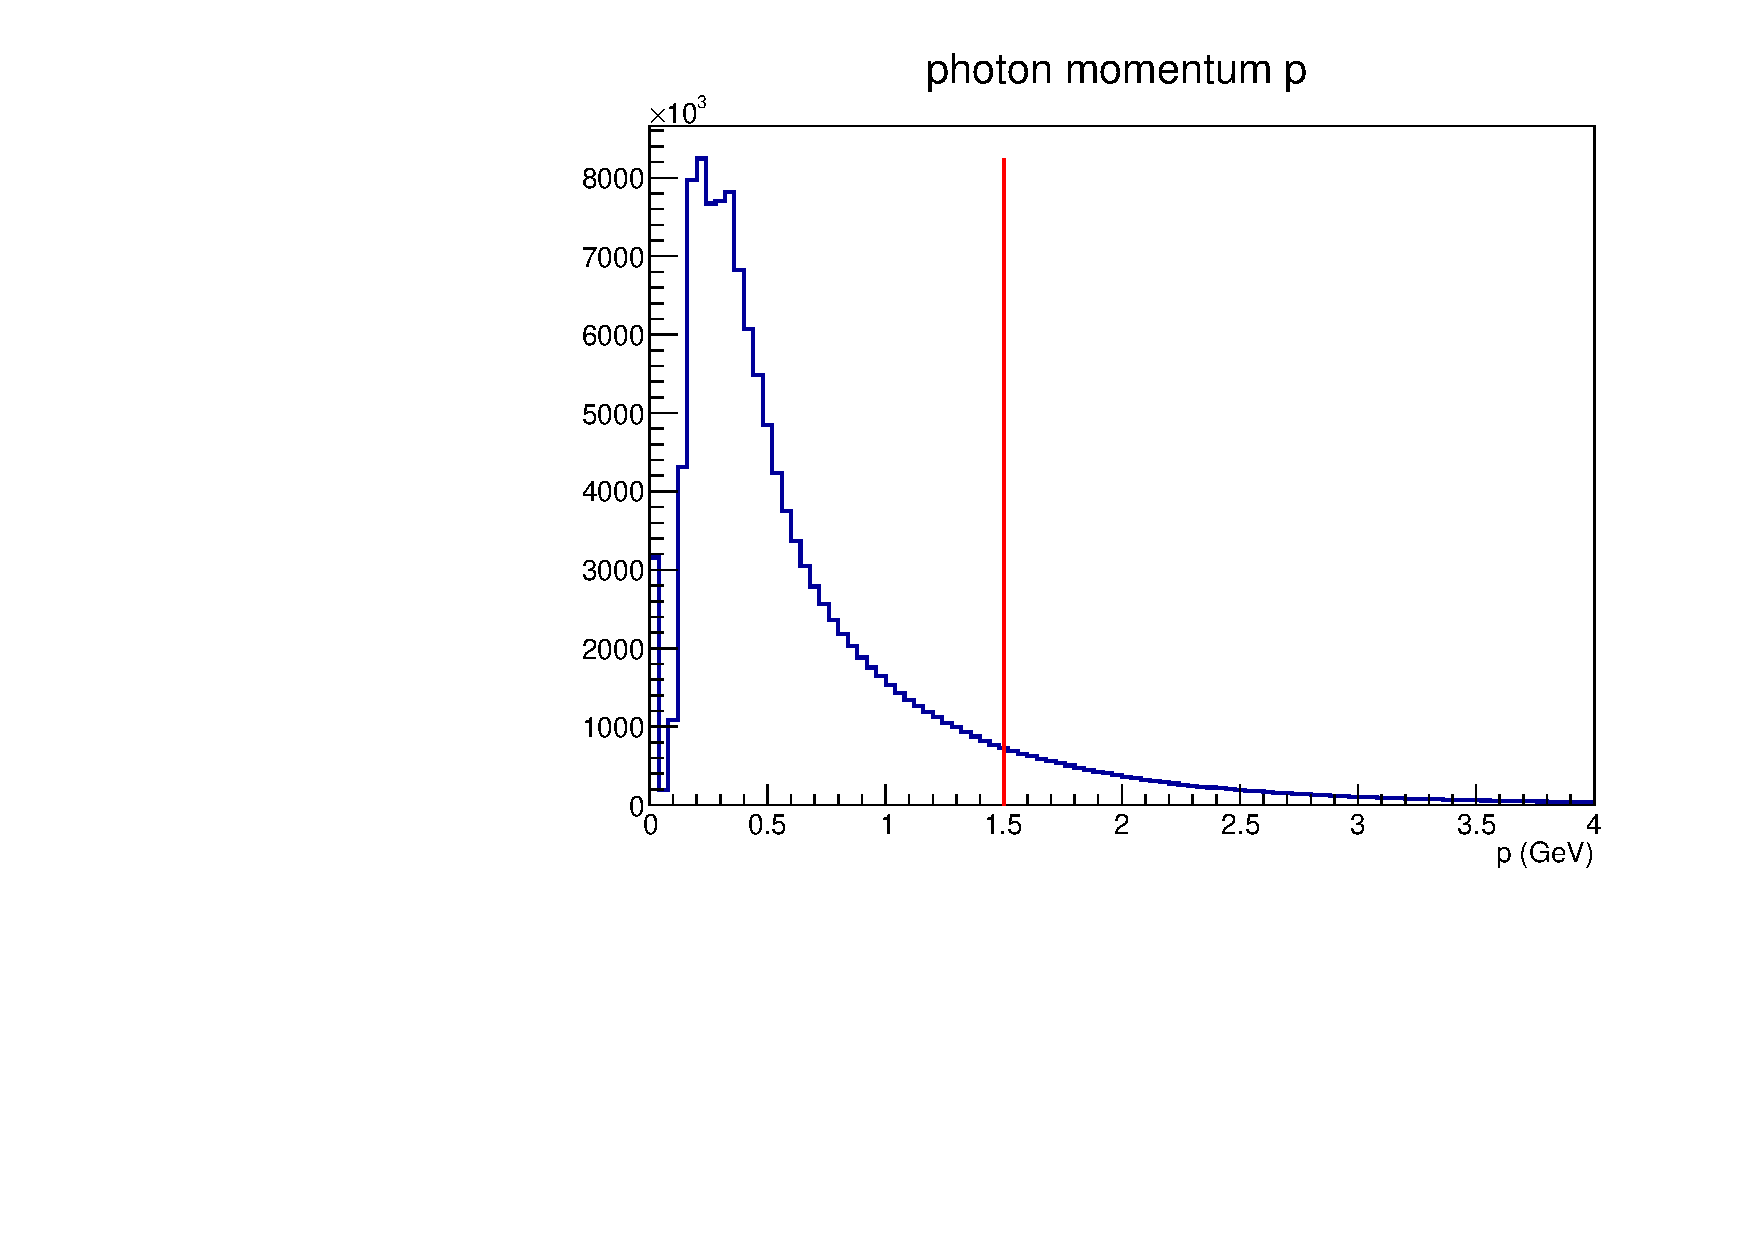
\includegraphics[width=\linewidth]{figures/dvcs_candidate_photon_p.pdf}
    \end{minipage}

    \begin{minipage}{0.3\linewidth}
        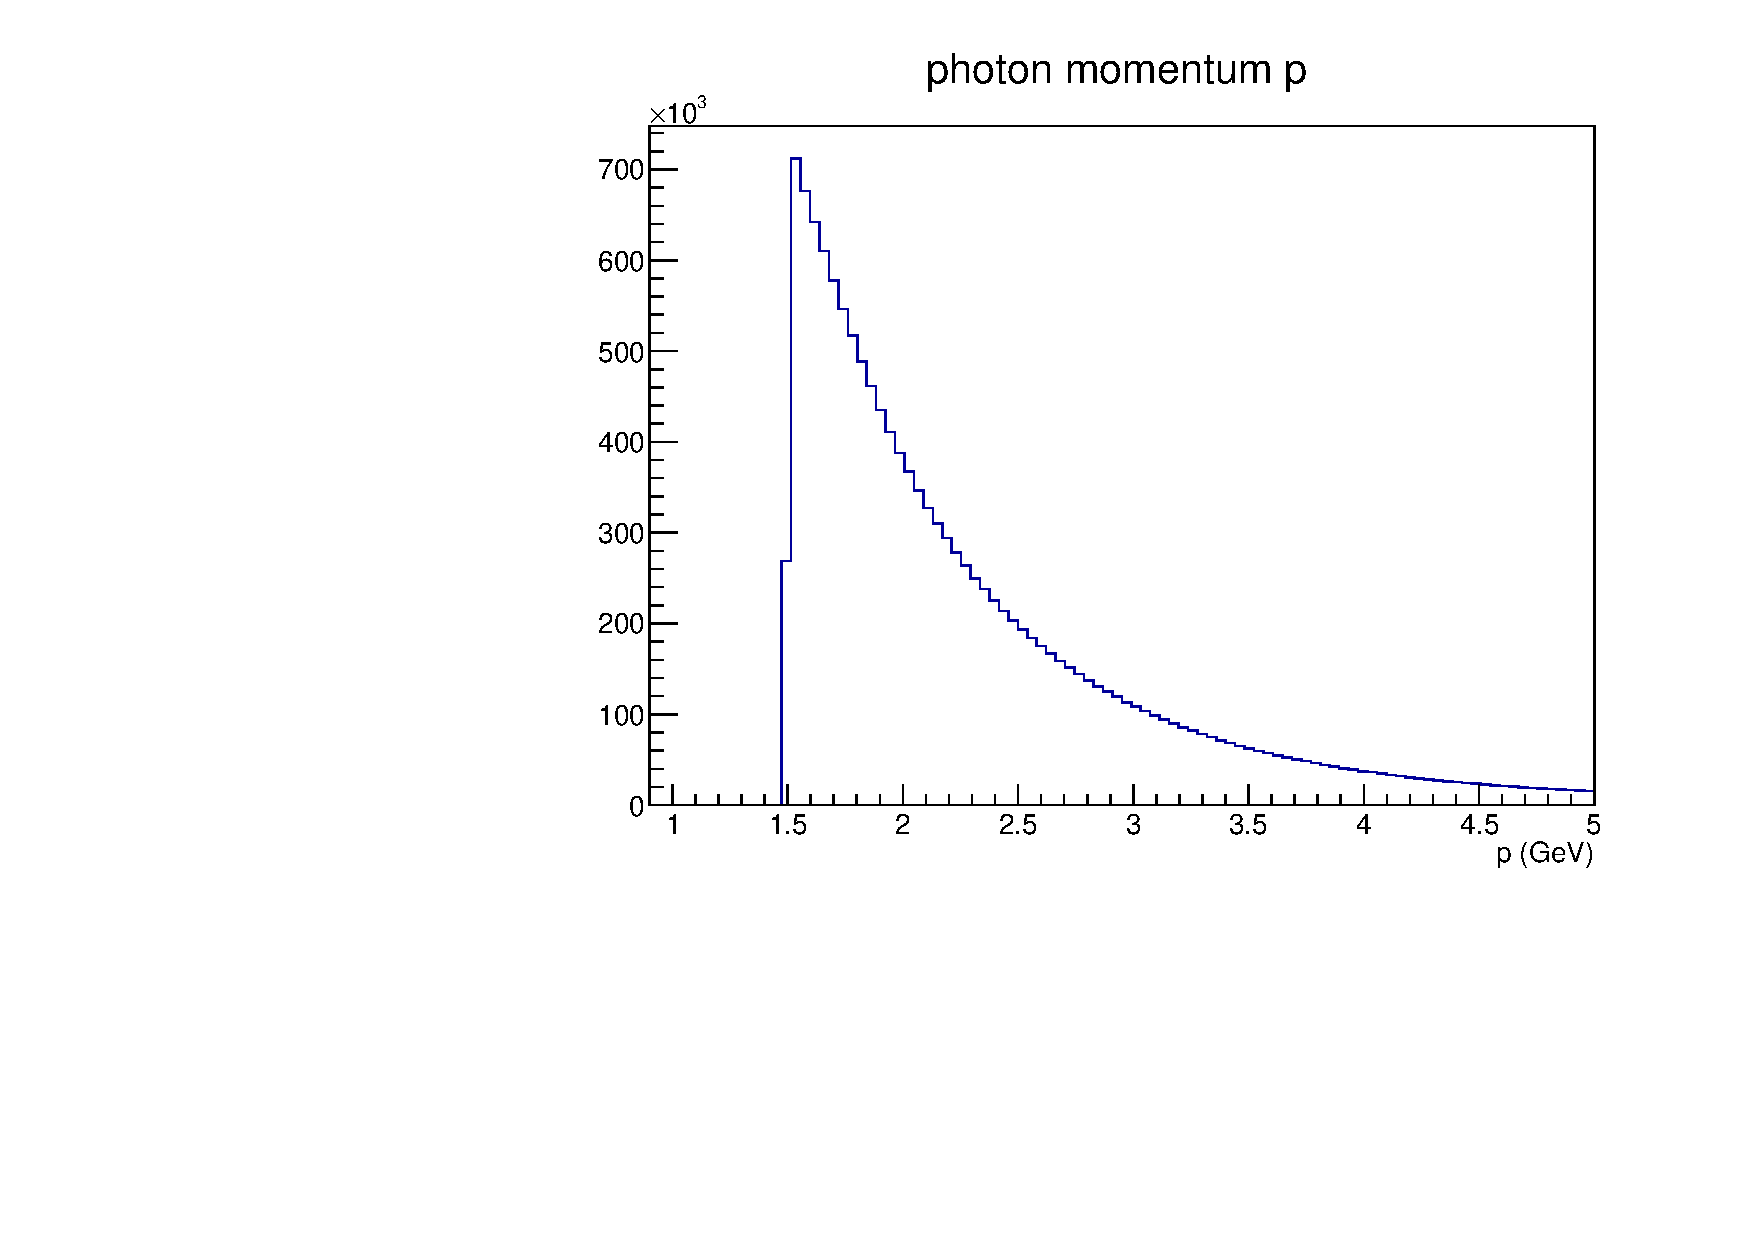
\includegraphics[width=\linewidth]{figures/photon_p_elecmom_cut.pdf}
    \end{minipage}
    \begin{minipage}{0.3\linewidth}
        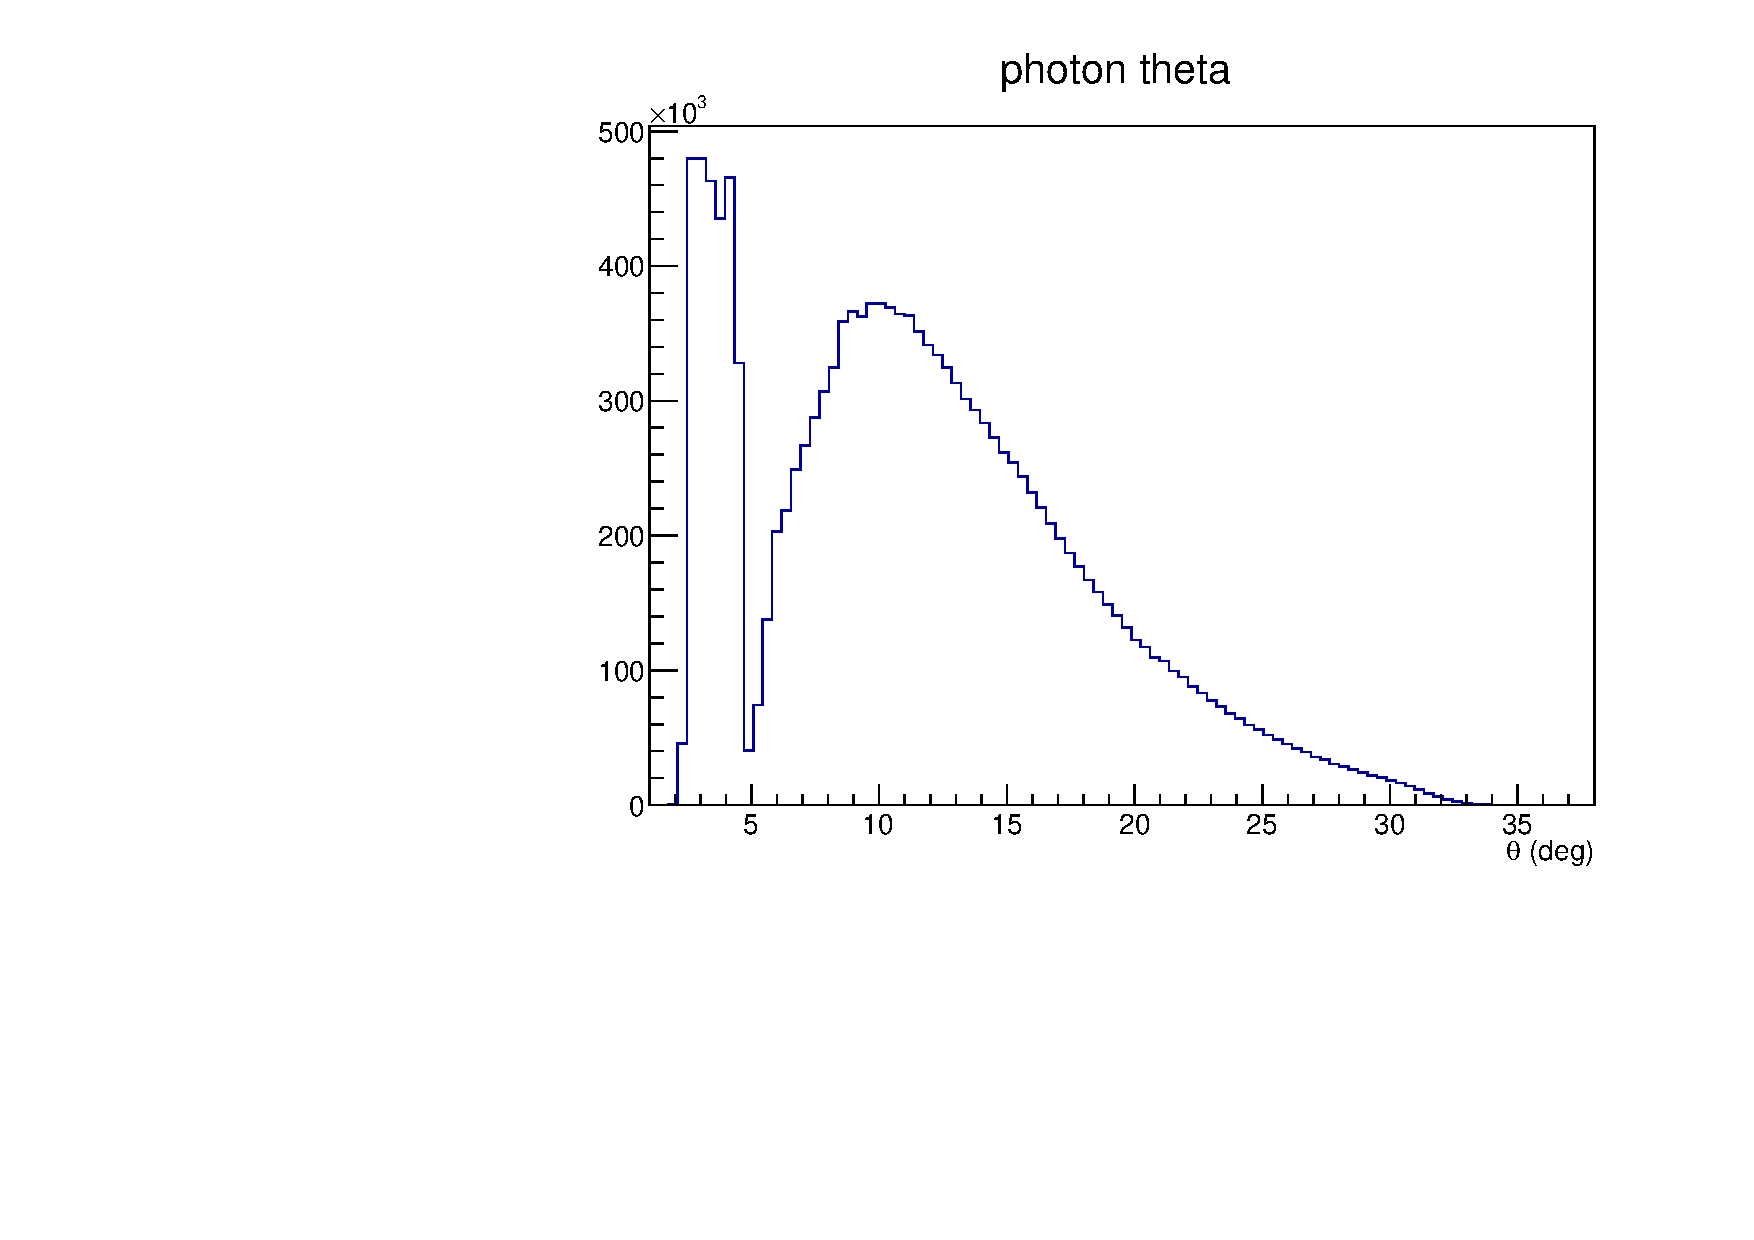
\includegraphics[width=\linewidth]{figures/photon_theta_elecmom_cut.pdf}
    \end{minipage}
    \begin{minipage}{0.3\linewidth}
        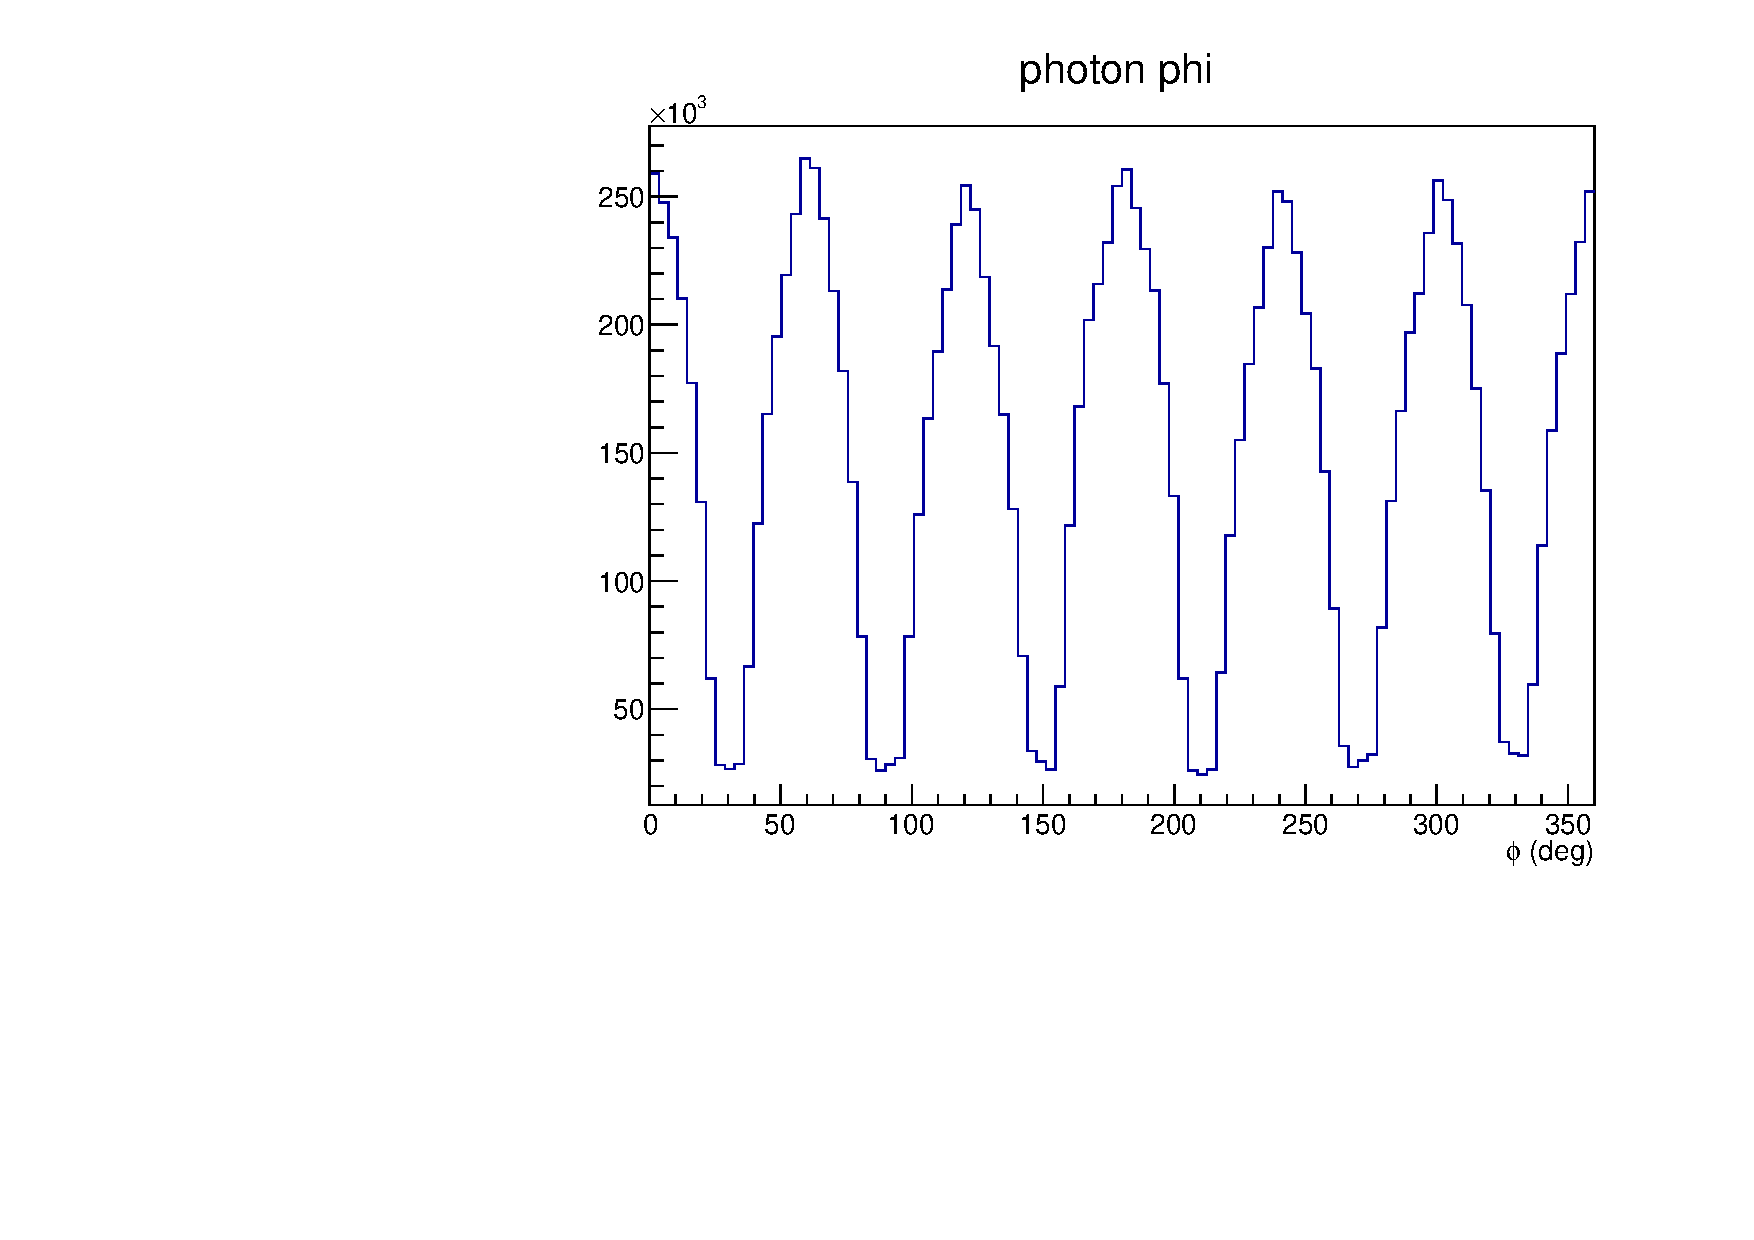
\includegraphics[width=\linewidth]{figures/photon_phi_elecmom_cut.pdf}
    \end{minipage}
\end{frame}


\begin{frame}{AHDC track selection}
    \begin{itemize}
        \item We require the detection of 1 electron and 1 photon
        \item The track quality should be good : $\mbox{nb. hits } \ge 7$, $\chi^2 < 8$
        \item The AHDC is not in the Event Builder yet, so we select $^4\mbox{He}$ based on their big deposited energy : $\Sigma \mbox{\footnotesize ADC} > 10000 $
    \end{itemize}

    \centering
    \vspace{0.2cm}

    
    \begin{minipage}{0.3\linewidth}
        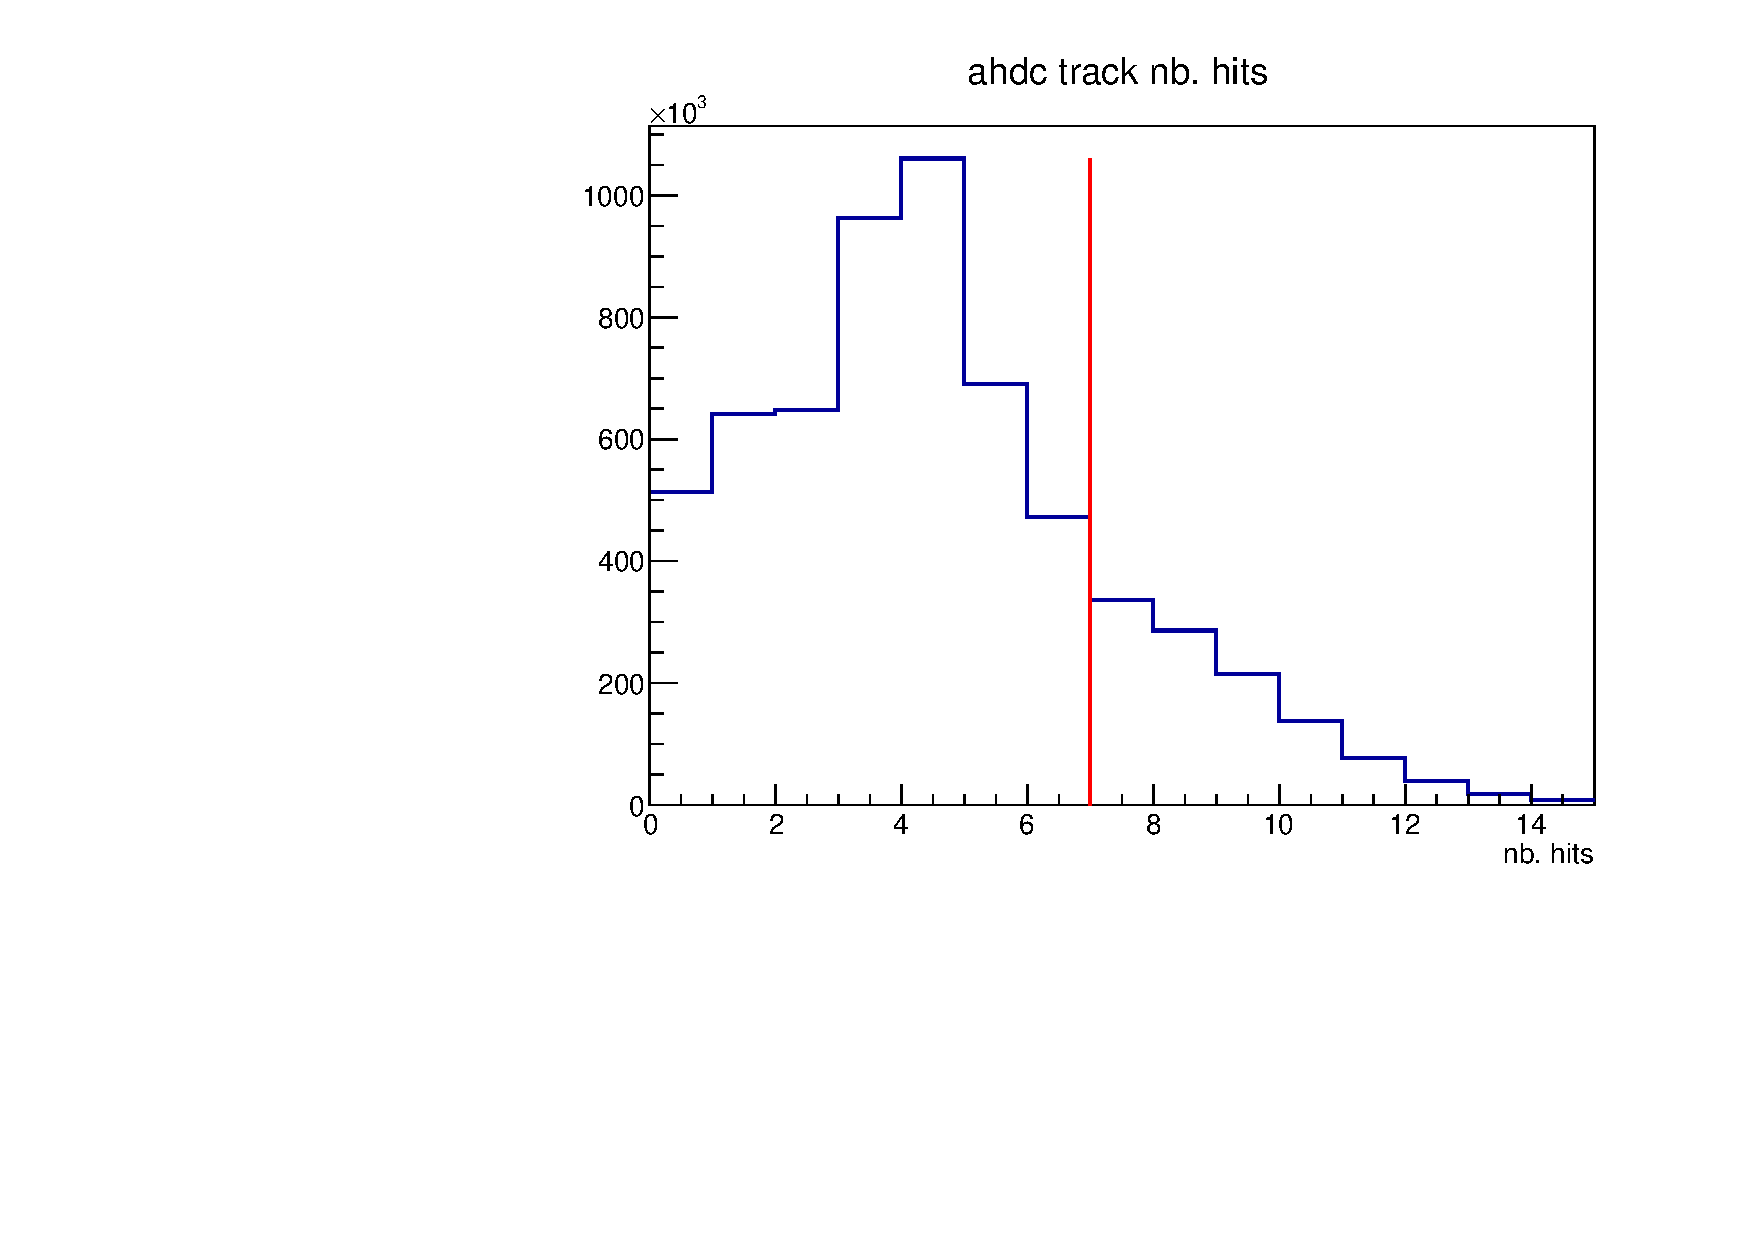
\includegraphics[width=\linewidth]{figures/dvcs_candidate_ahdc_track_nhits.pdf}
    \end{minipage}
    \begin{minipage}{0.3\linewidth}
        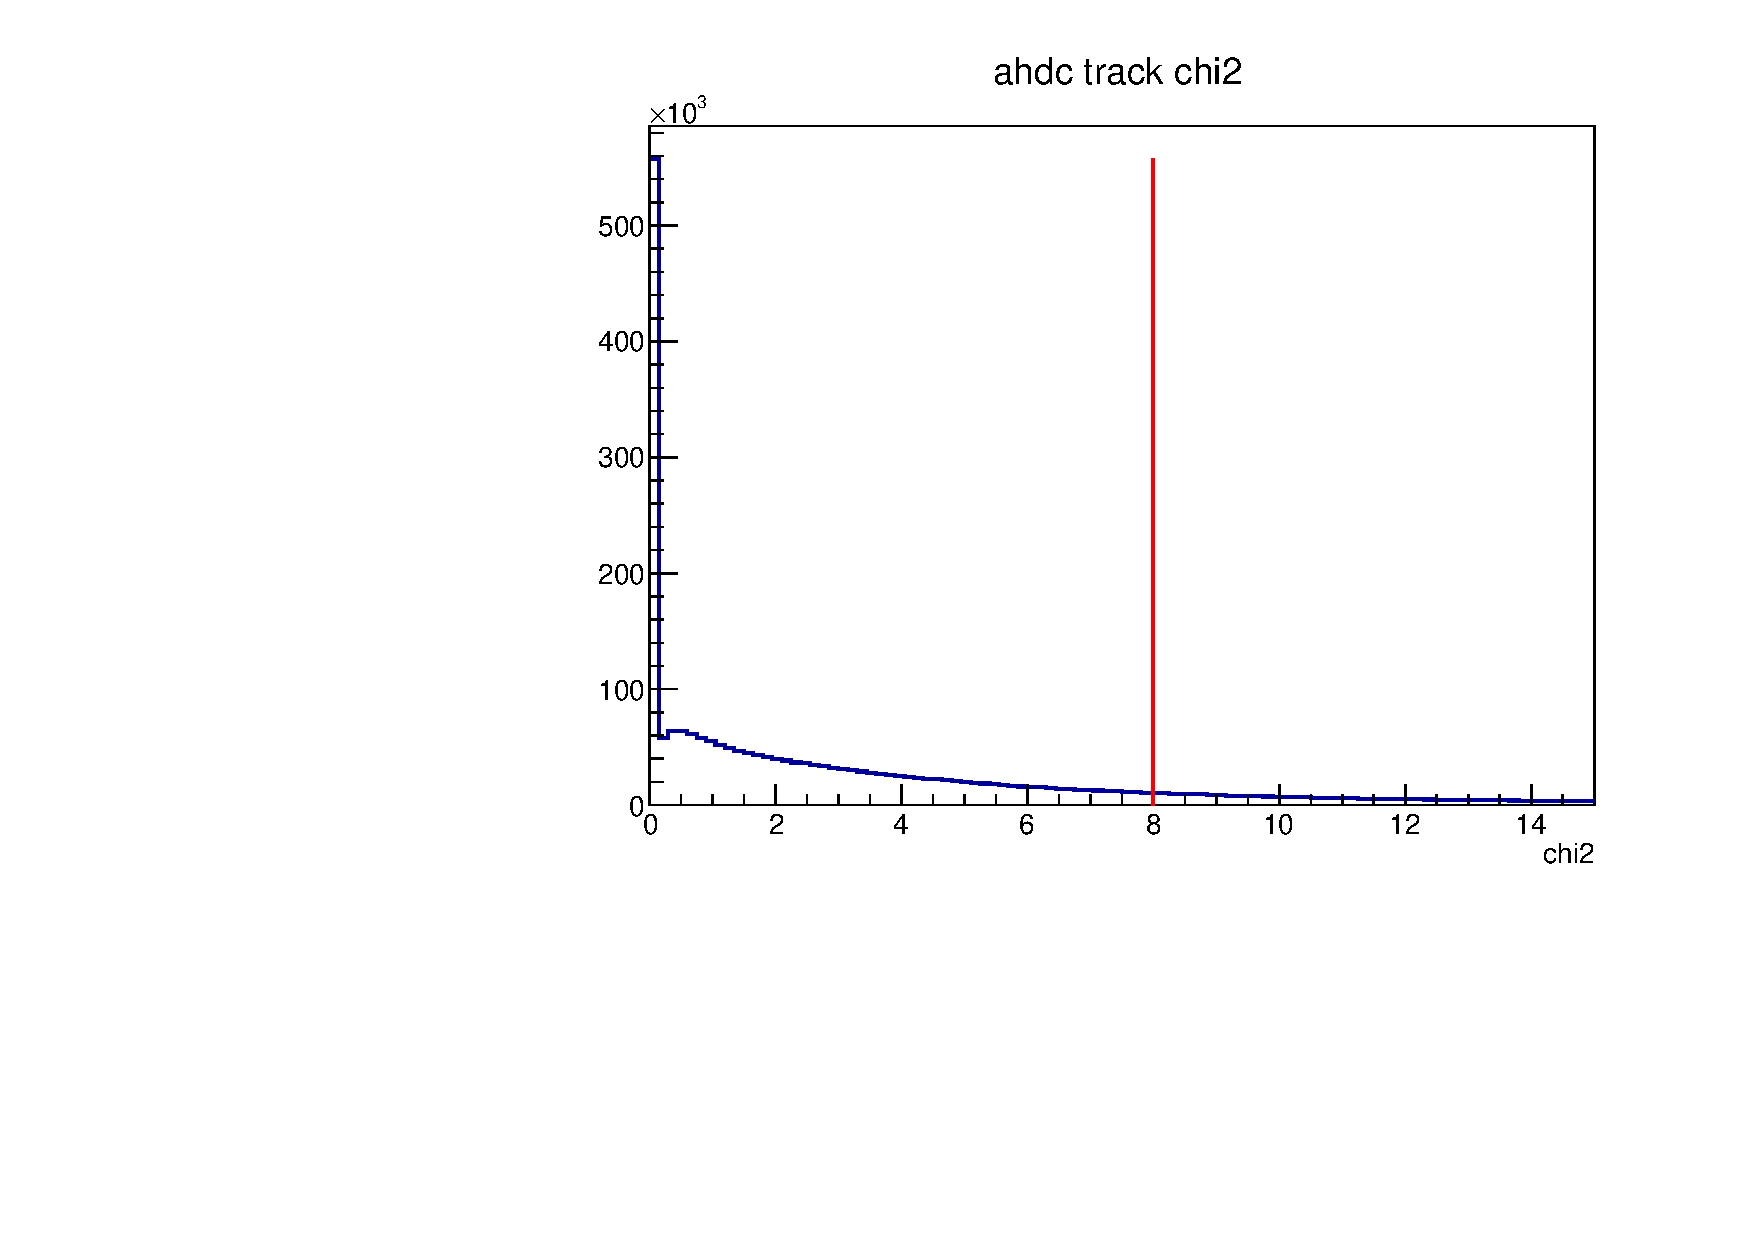
\includegraphics[width=\linewidth]{figures/dvcs_candidate_ahdc_track_chi2.pdf}
    \end{minipage}
    \begin{minipage}{0.3\linewidth}
        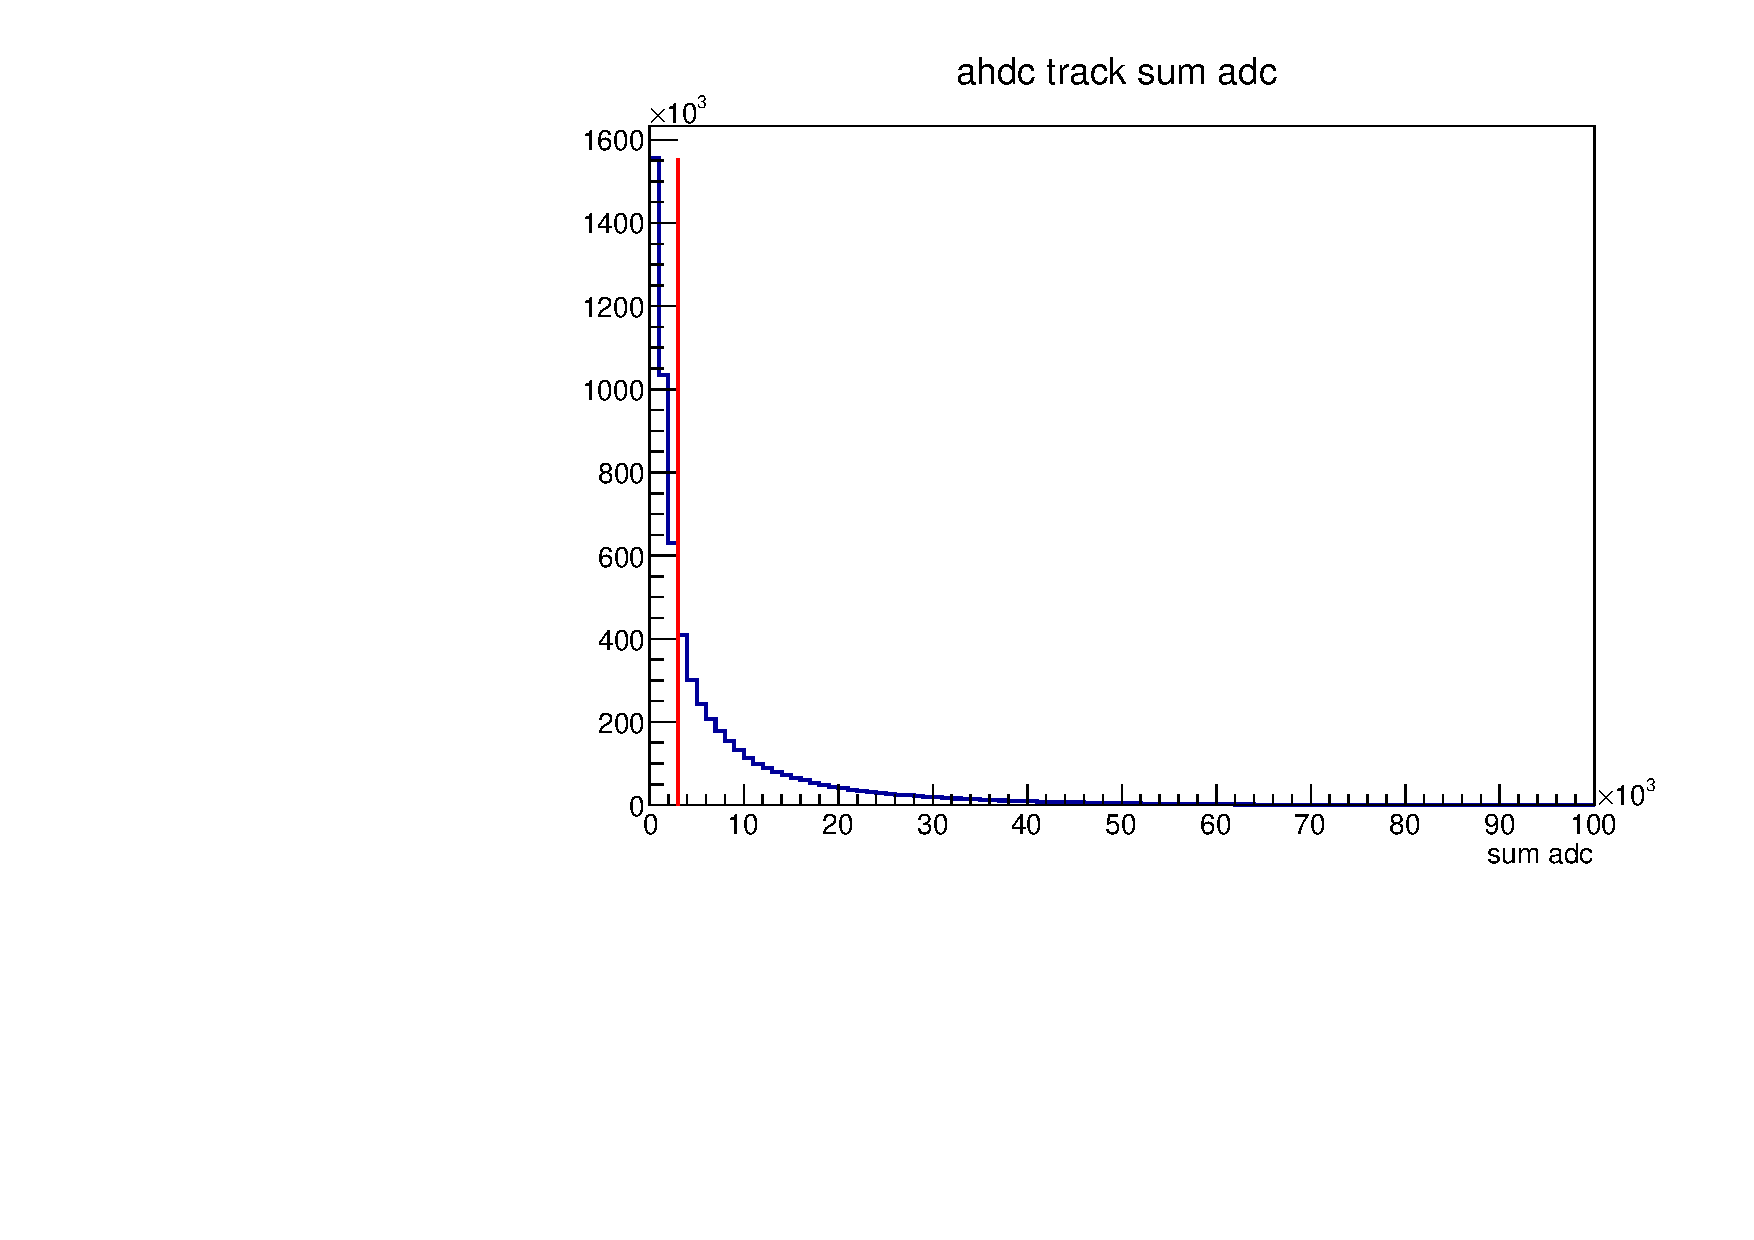
\includegraphics[width=\linewidth]{figures/dvcs_candidate_ahdc_track_sum_adc.pdf}
    \end{minipage}
    \begin{minipage}{0.3\linewidth}
        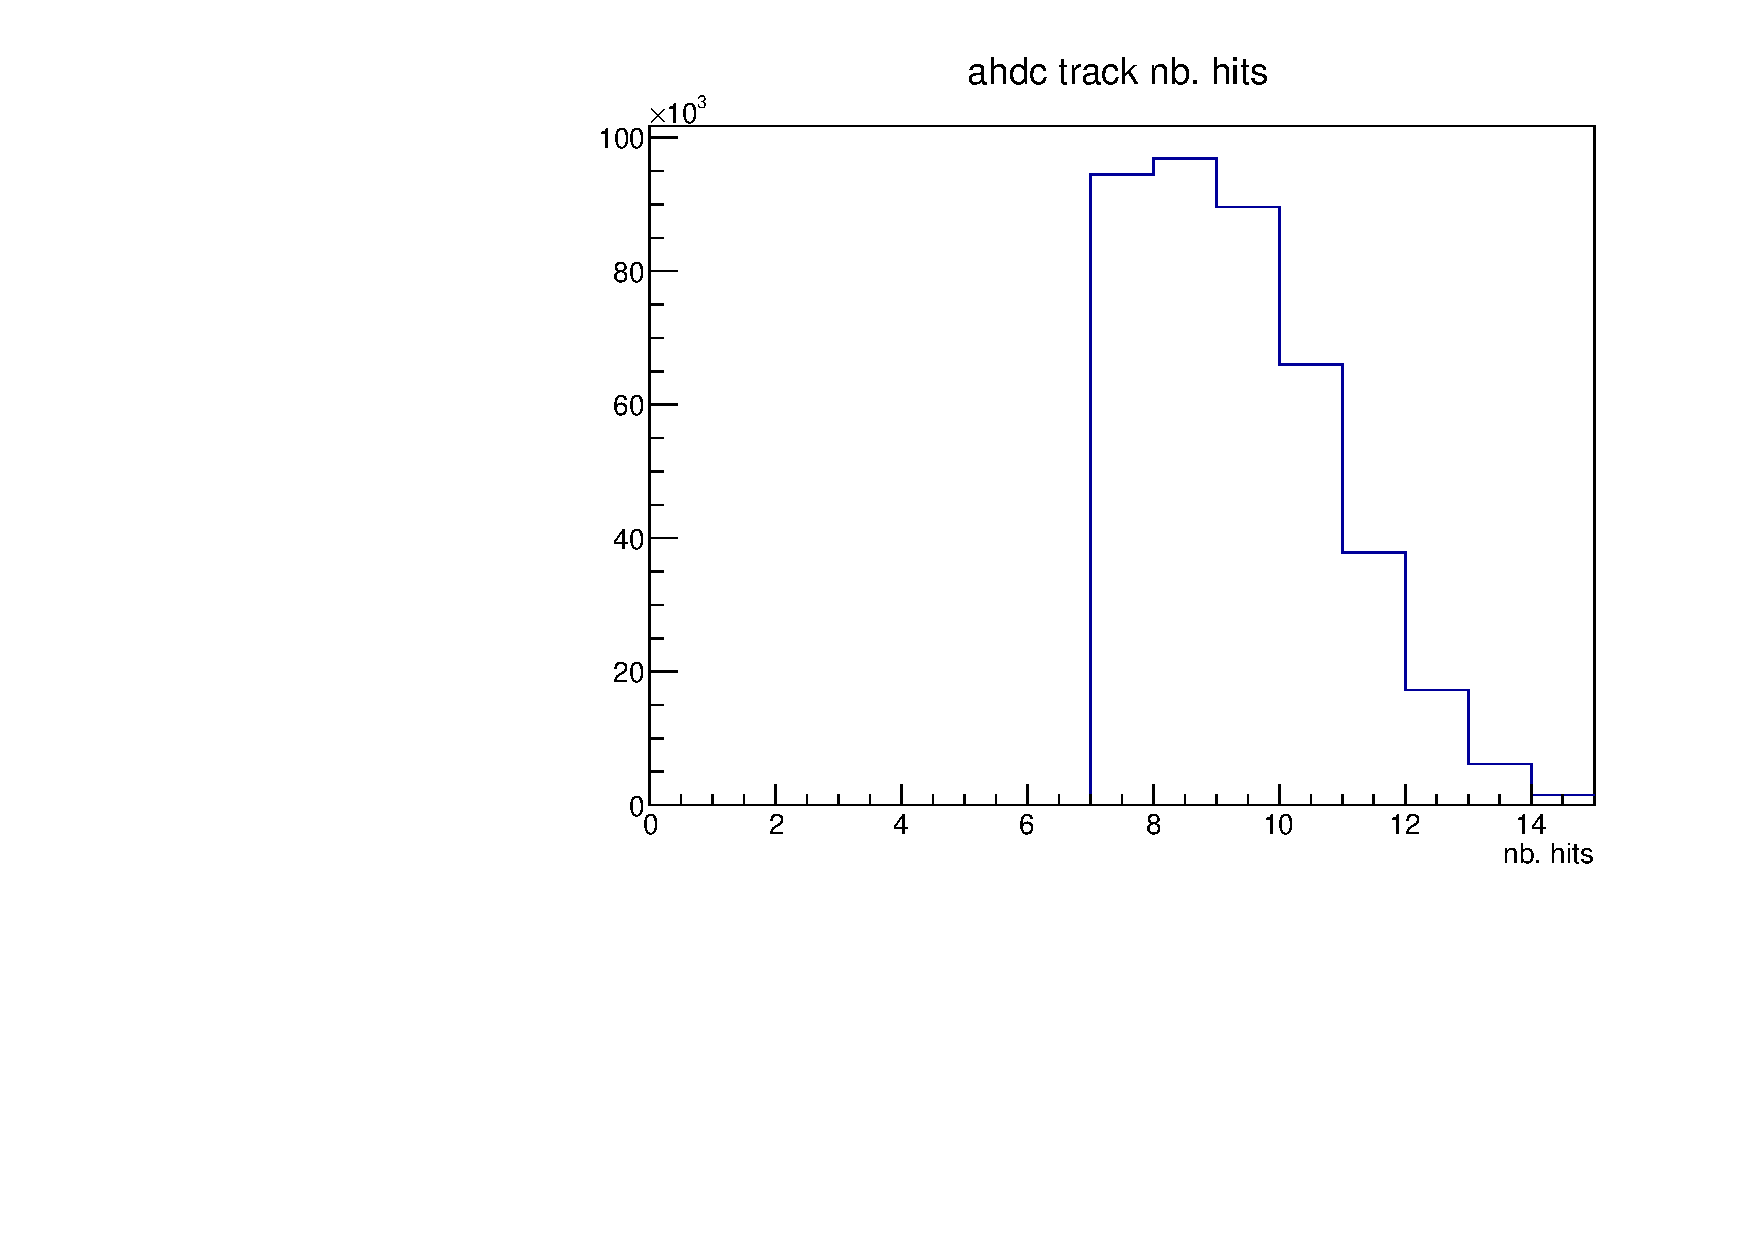
\includegraphics[width=\linewidth]{figures/ahdc_track_nb_hits_quality_cut.pdf}
    \end{minipage}
    \begin{minipage}{0.3\linewidth}
        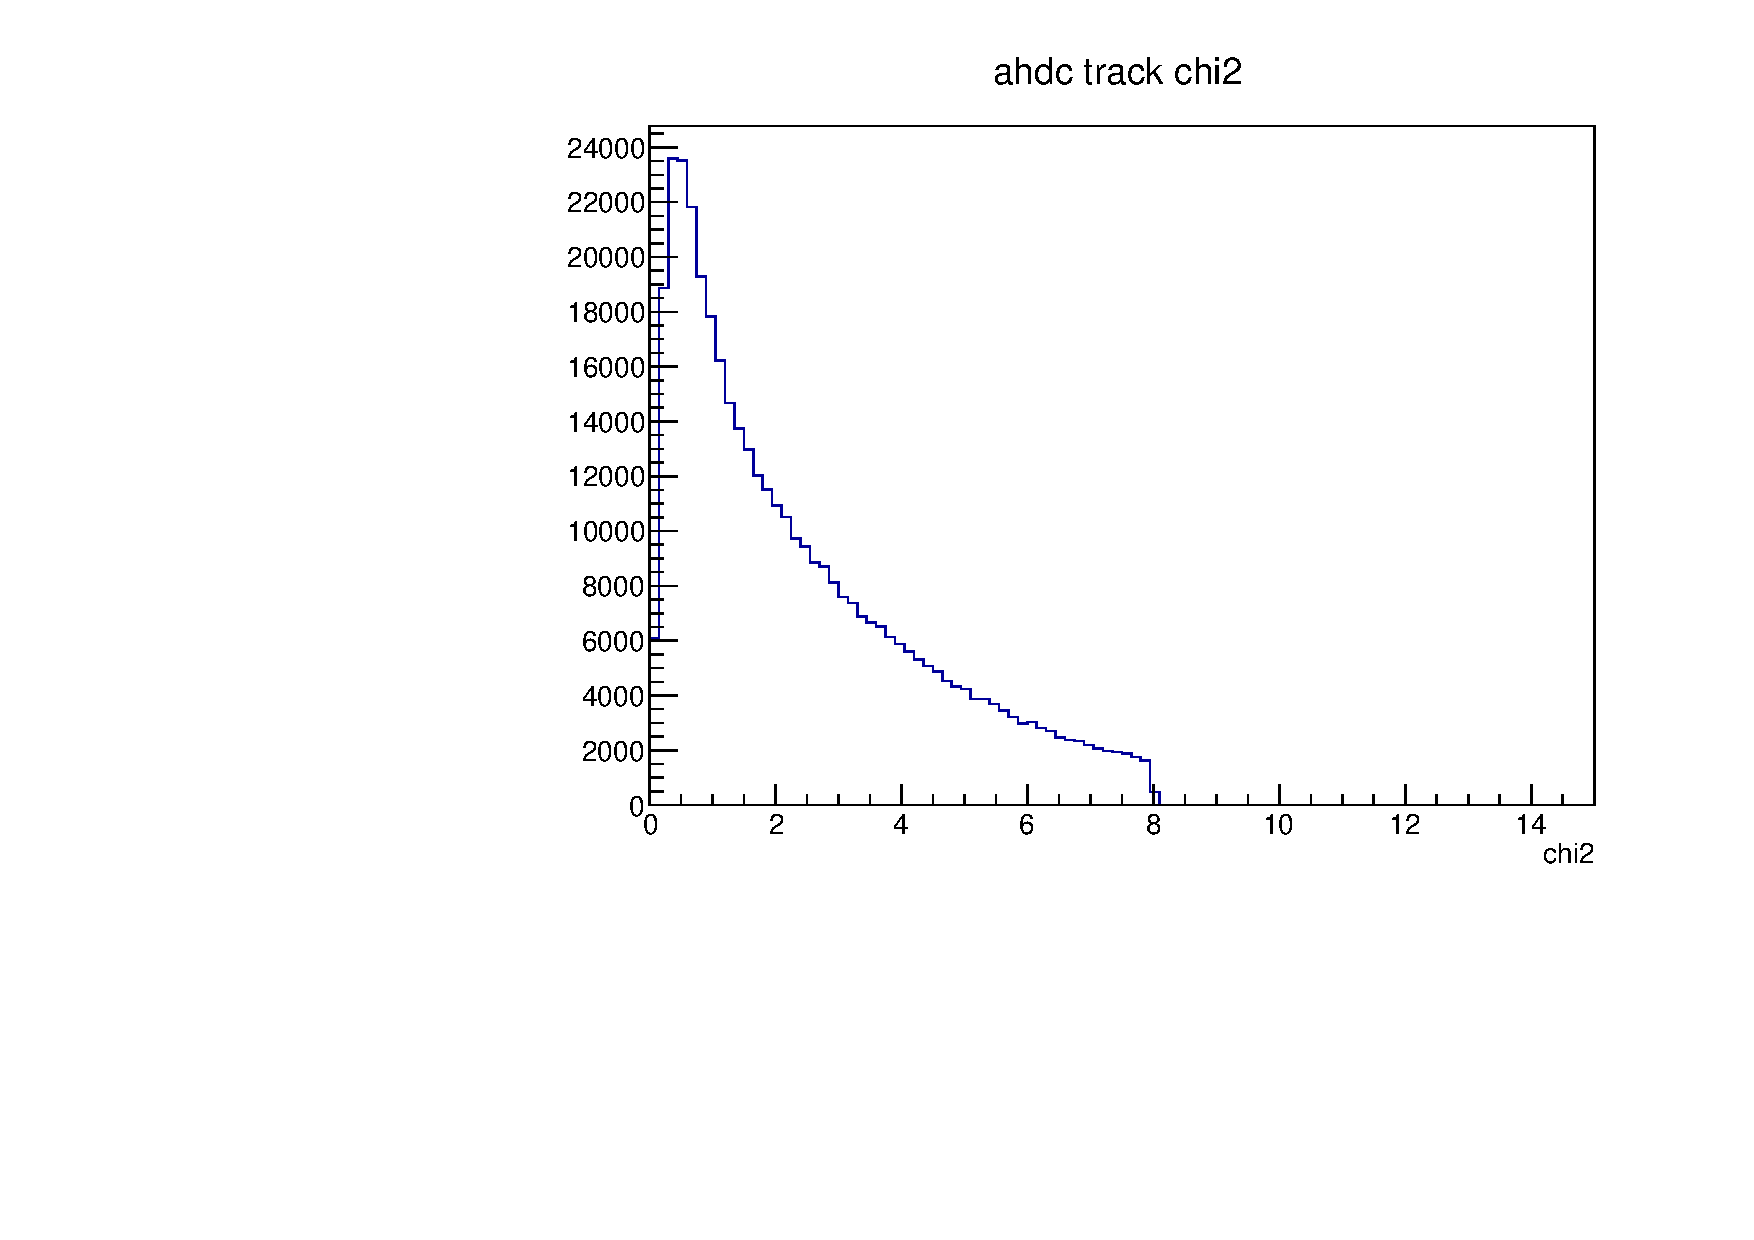
\includegraphics[width=\linewidth]{figures/ahdc_track_chi2_quality_cut.pdf}
    \end{minipage}
    \begin{minipage}{0.3\linewidth}
        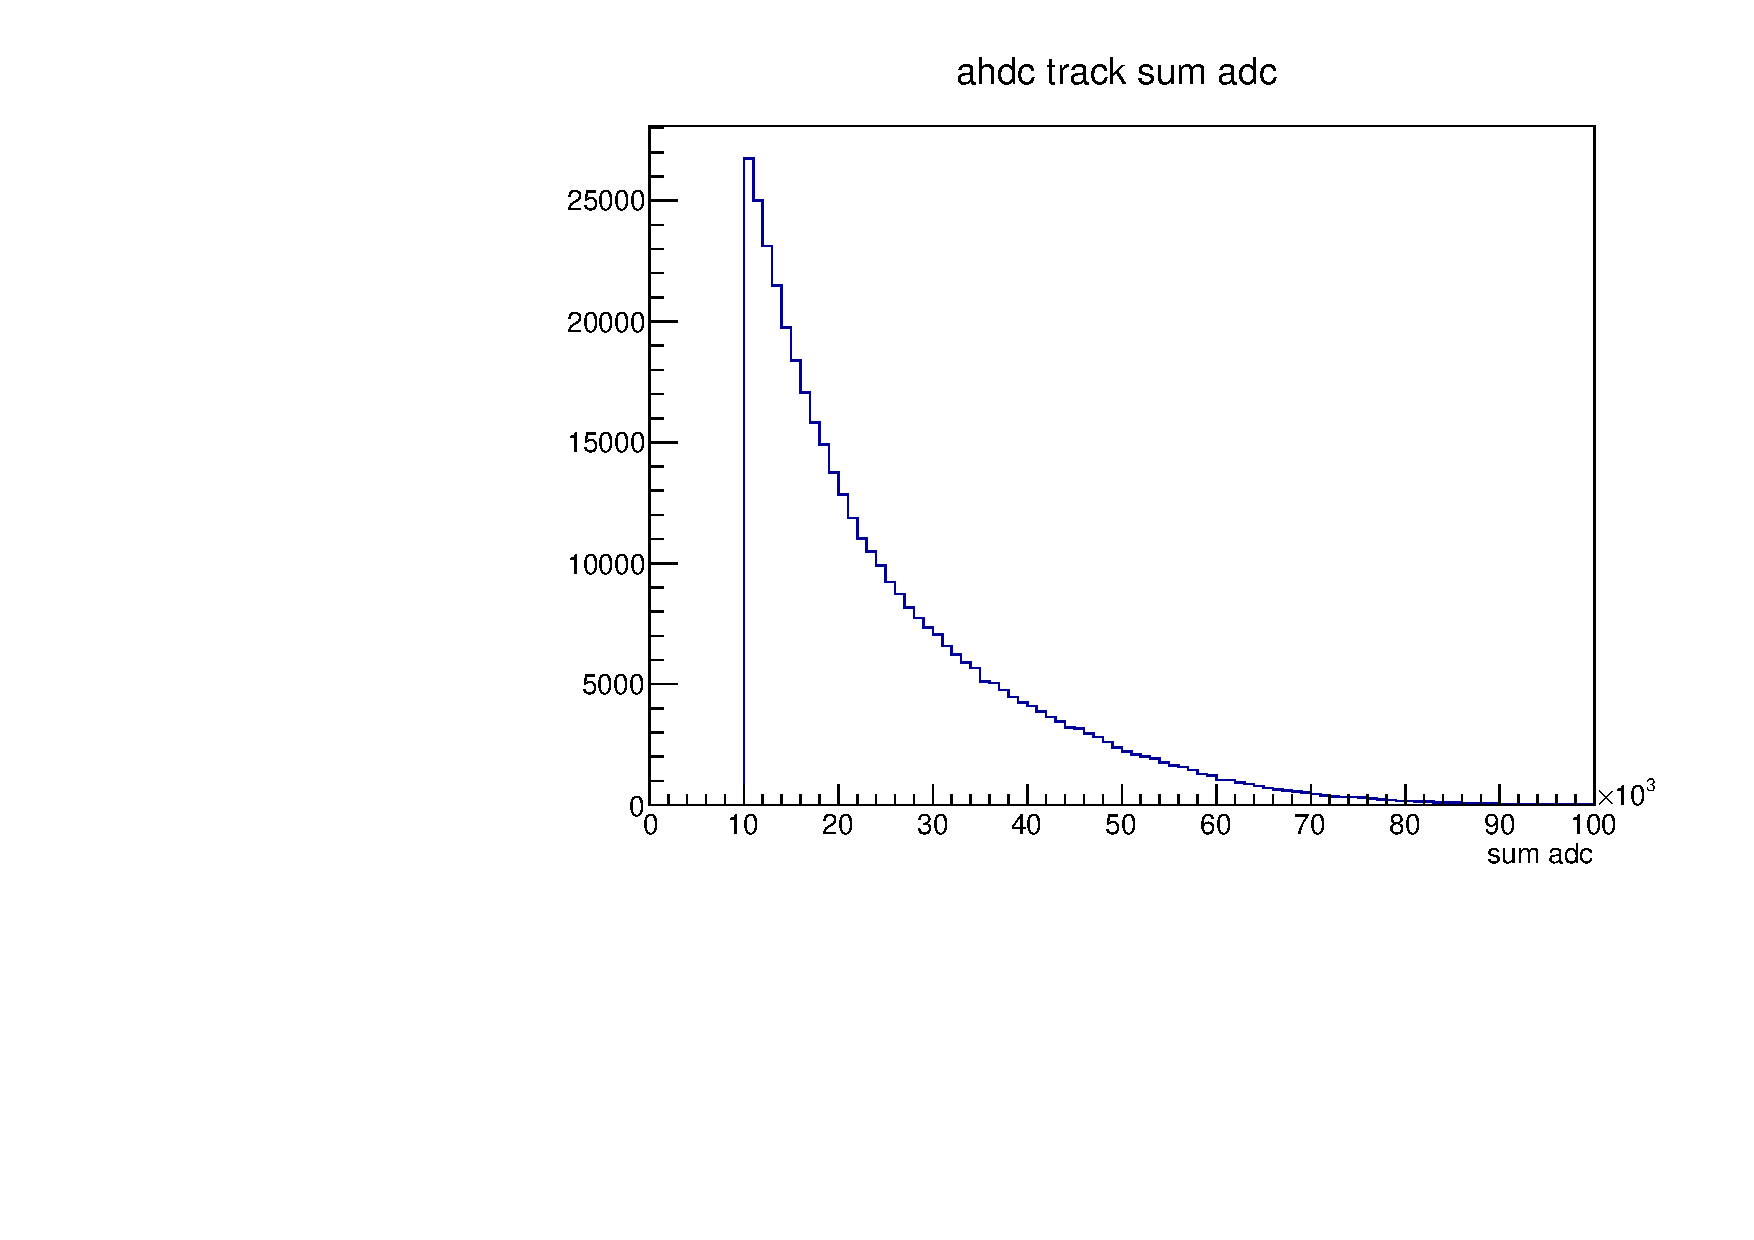
\includegraphics[width=\linewidth]{figures/ahdc_track_sum_adc_quality_cut.pdf}
    \end{minipage}
    
\end{frame}

\begin{frame}{AHDC track kinematics}

    \begin{itemize}
        \item The AHDC currently reconstructs p/q, so we correct the momentum by multiplying it by 2 (the charge of $^4\mbox{He}$)
        \item The theta reconstruction is not very precise, so we don't use it here
    \end{itemize}

    \centering
    \vspace{0.4cm}

    \begin{minipage}{0.3\linewidth}
        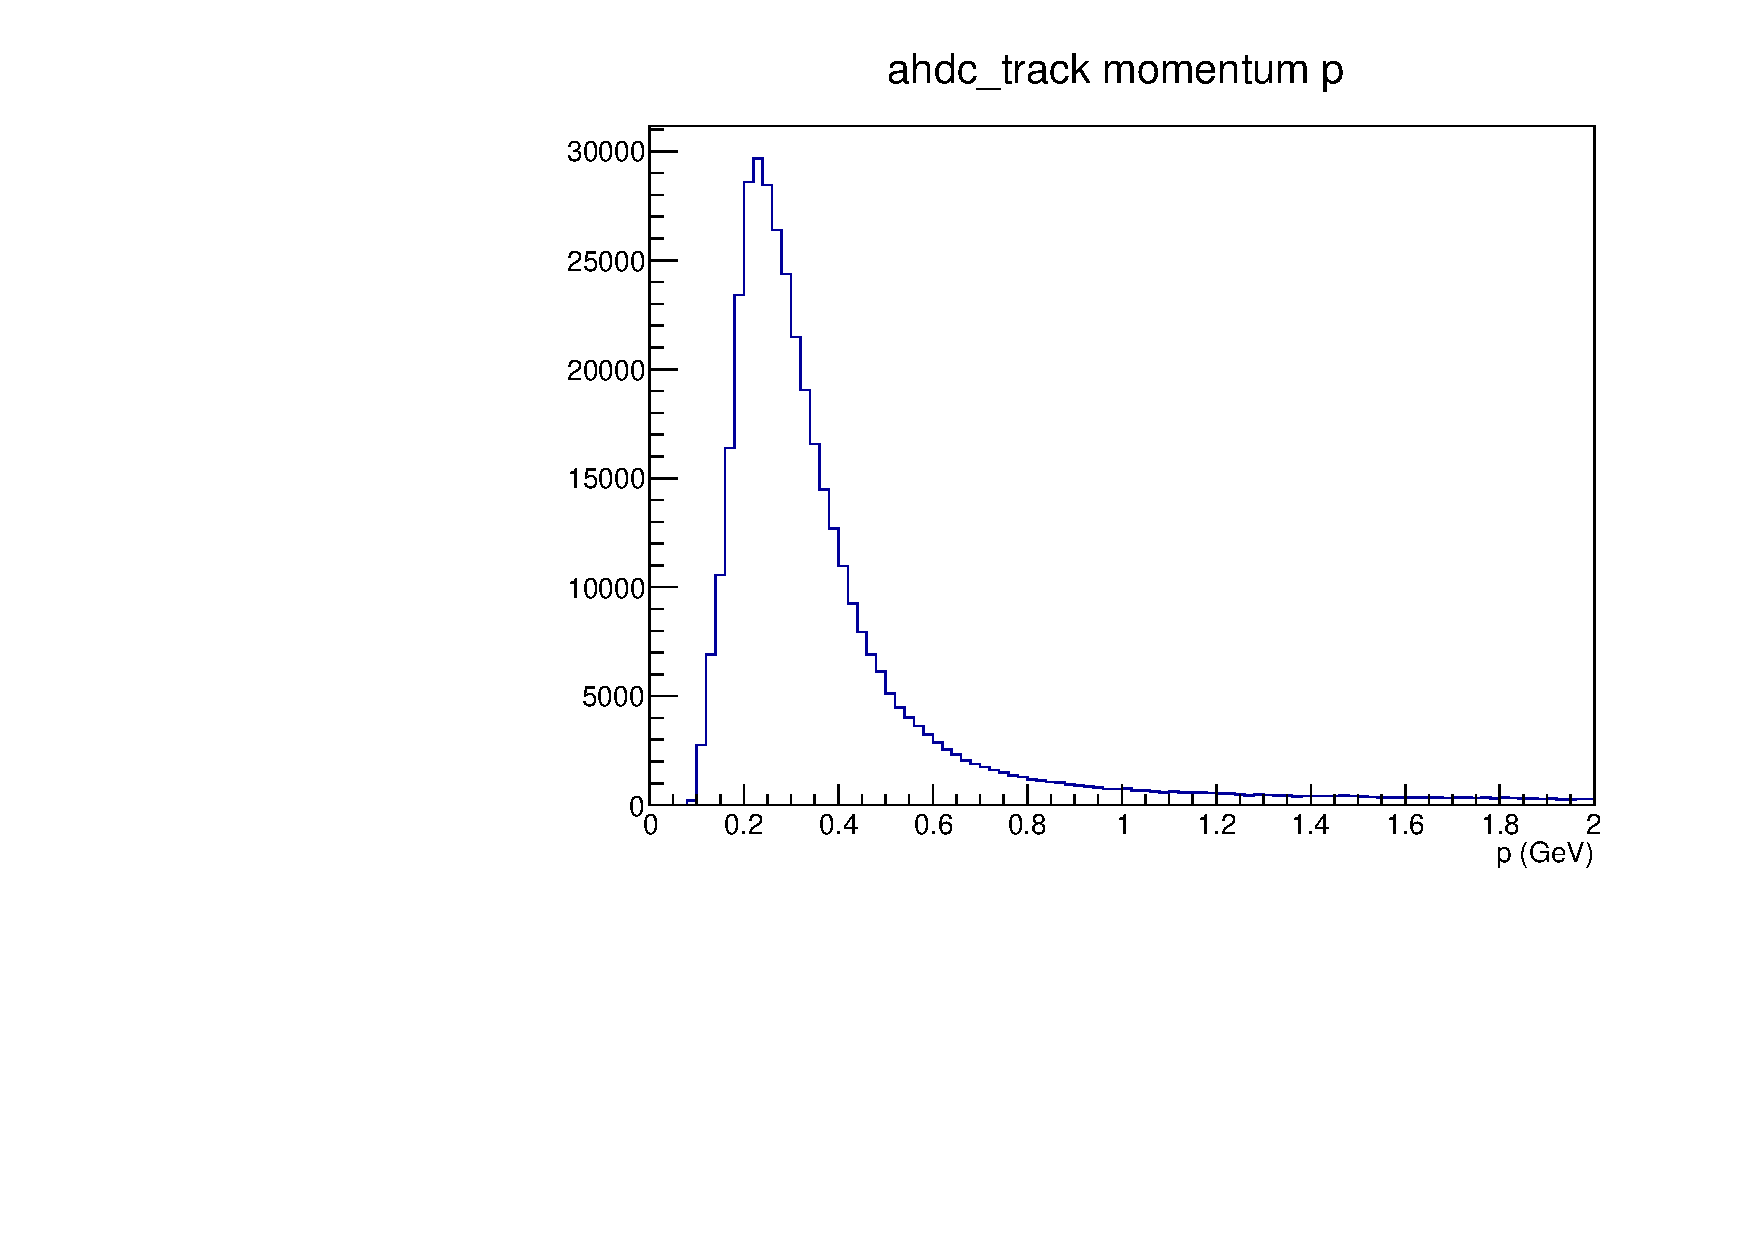
\includegraphics[width=\linewidth]{figures/ahdc_track_p_quality_cut.pdf}
    \end{minipage}
    \begin{minipage}{0.3\linewidth}
        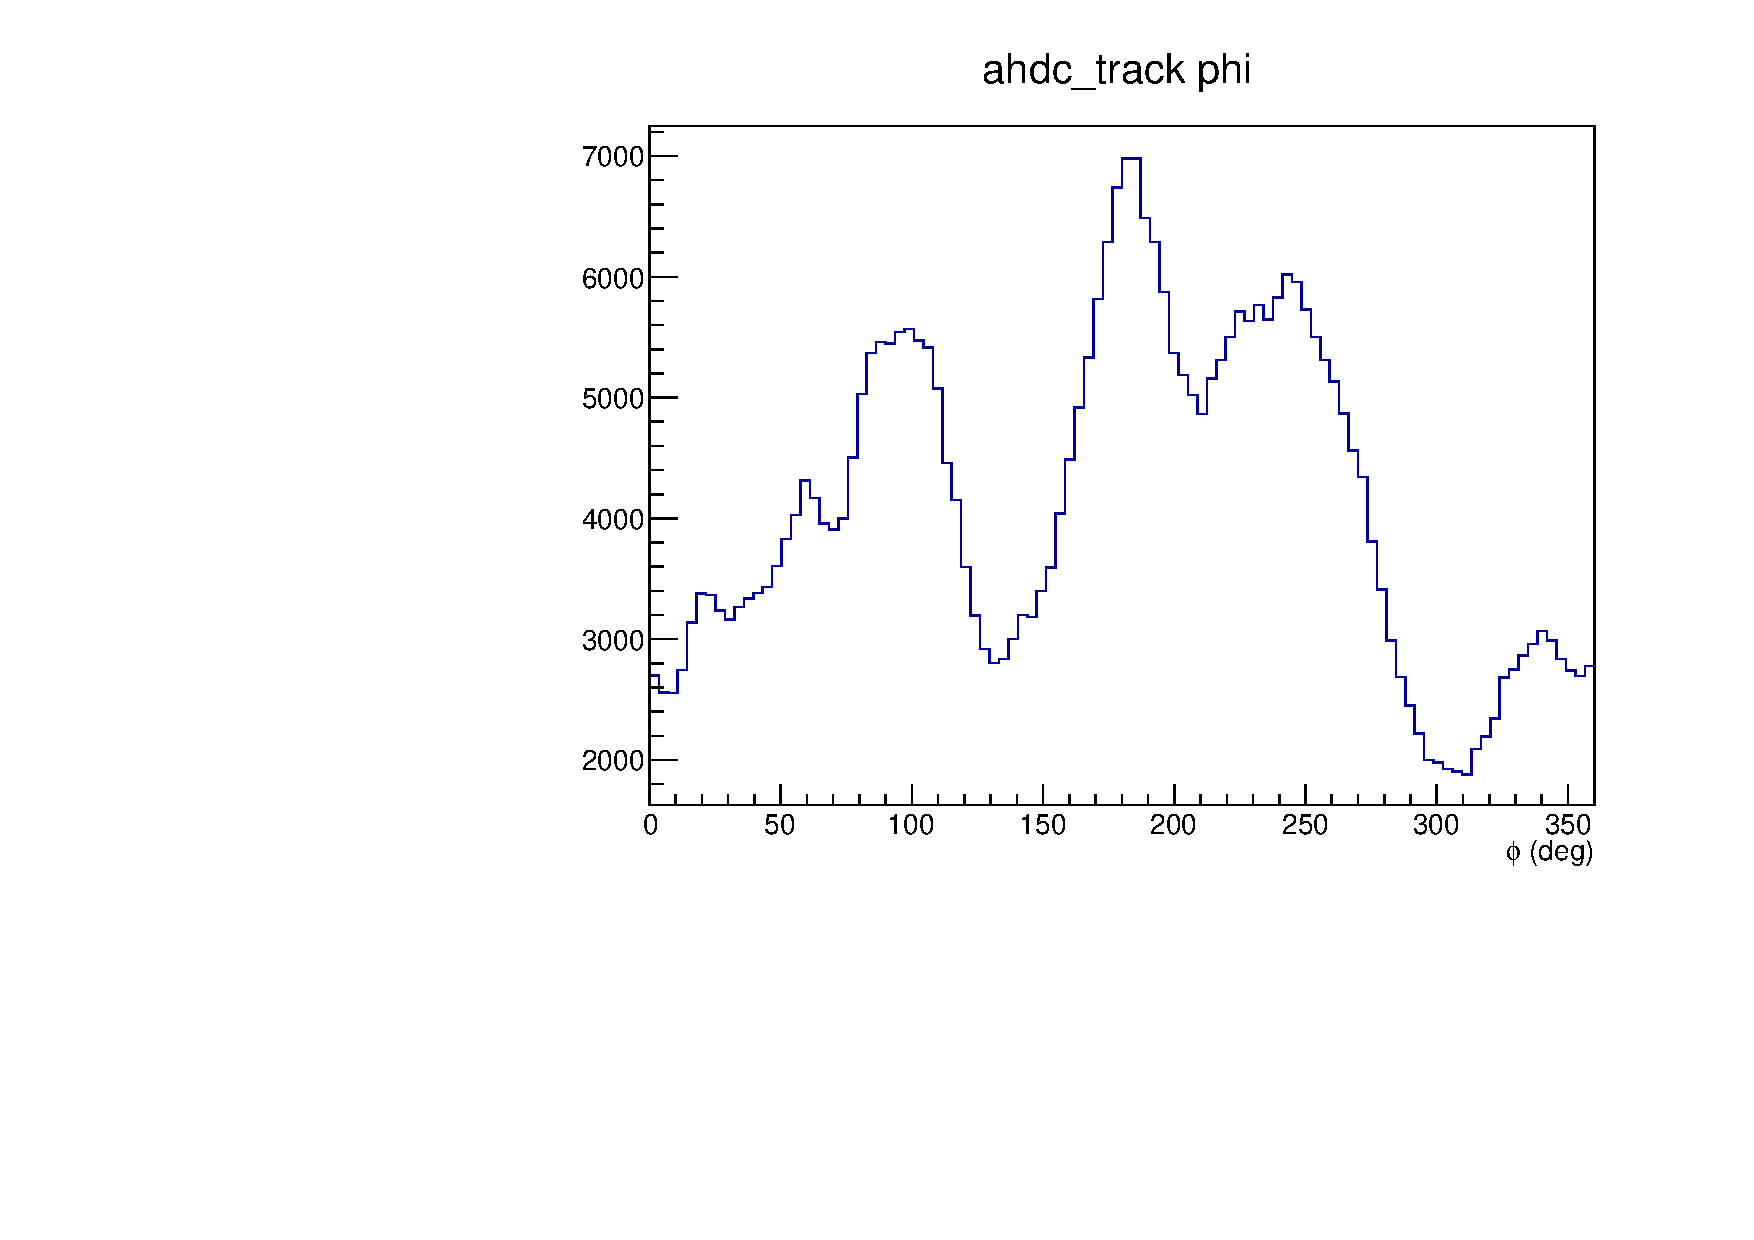
\includegraphics[width=\linewidth]{figures/ahdc_track_phi_quality_cut.pdf}
    \end{minipage}
    \begin{minipage}{0.3\linewidth}
        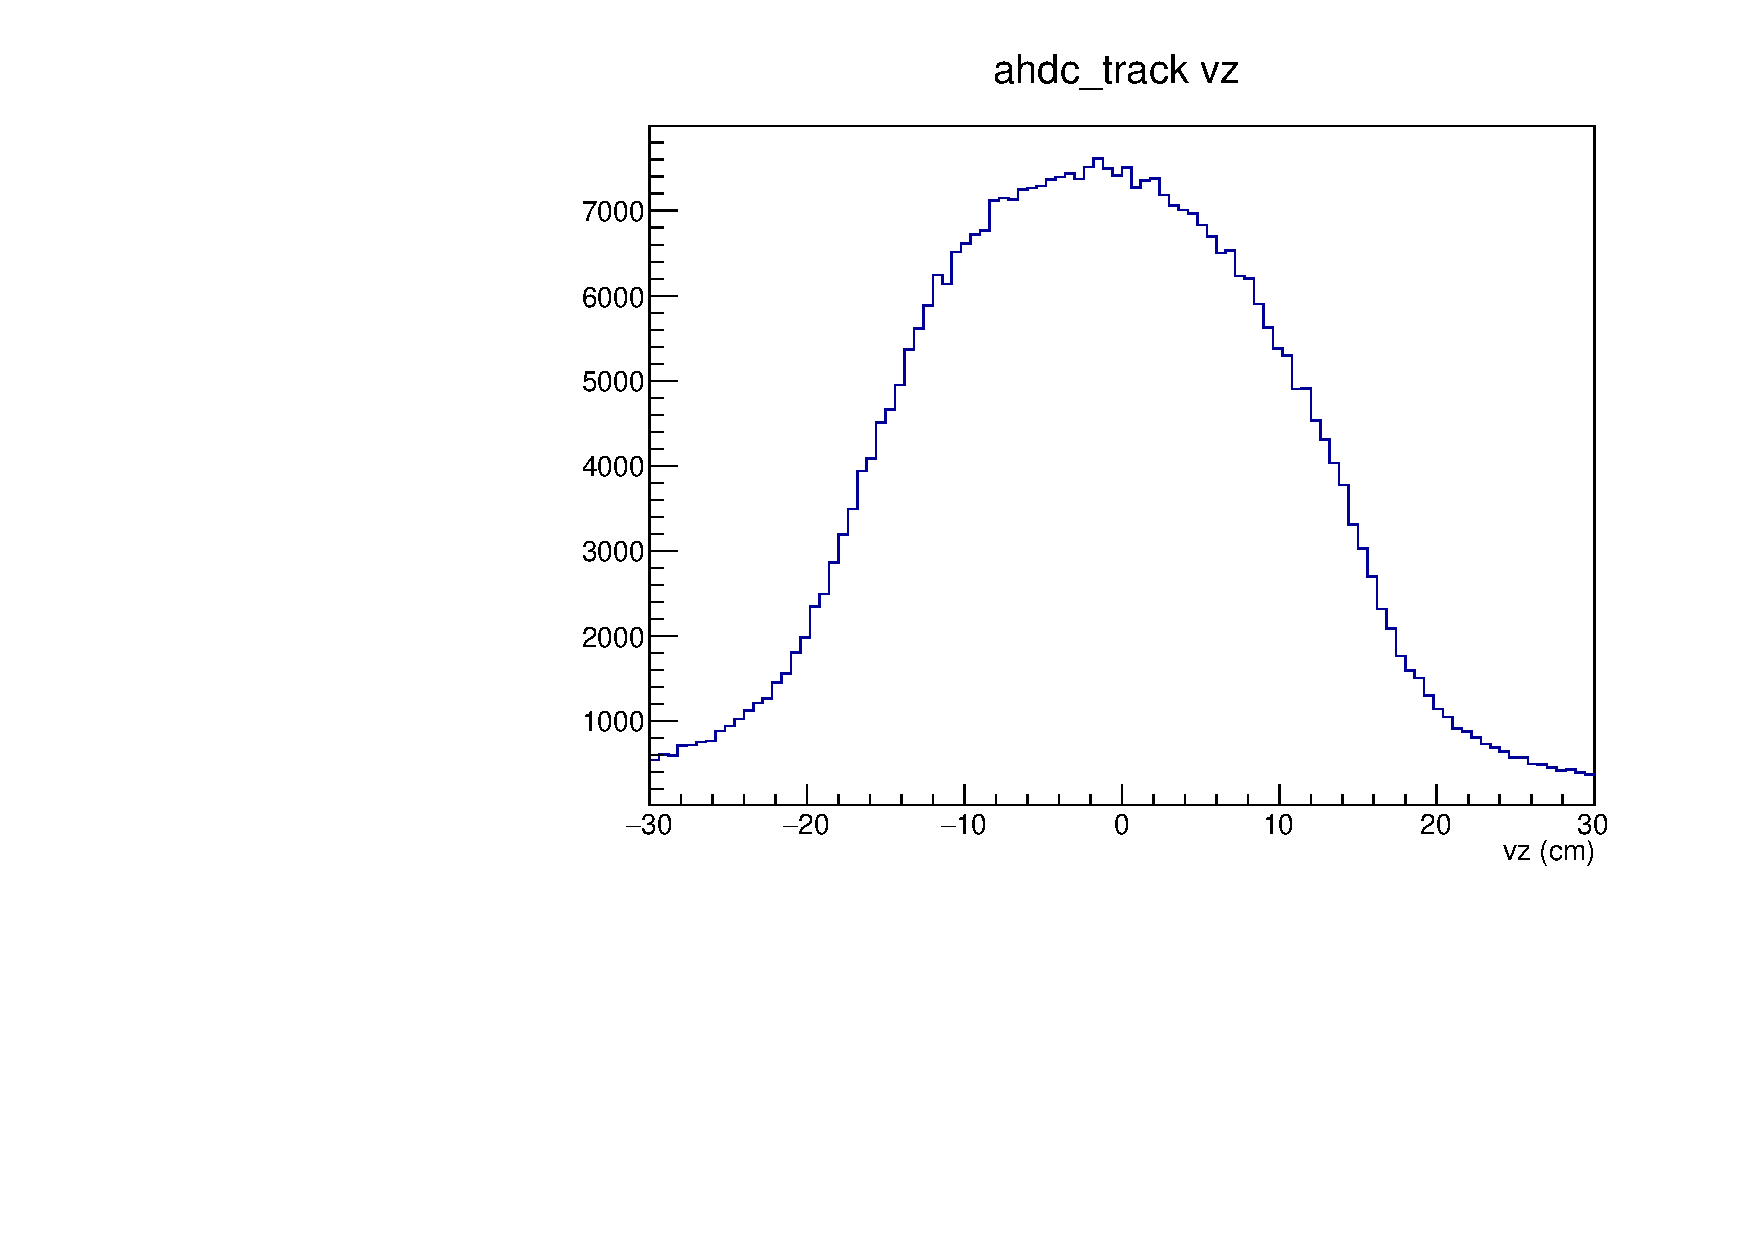
\includegraphics[width=\linewidth]{figures/ahdc_track_vz_quality_cut.pdf}
    \end{minipage}


\end{frame}

\begin{frame}{DVCS candidates}
    \begin{itemize}
        \item After selecting 1 electron, 1 photon and 1 AHDC track, we still need to verify the DVCS exclusivity distribution
        \item At this stage, only $\Delta \Phi$ has a clear peak
        \item I will apply : $|\Delta \Phi| < 15^\circ$
    \end{itemize}

    \centering
    \vspace{0.2cm}

    \begin{minipage}{0.3\linewidth}
        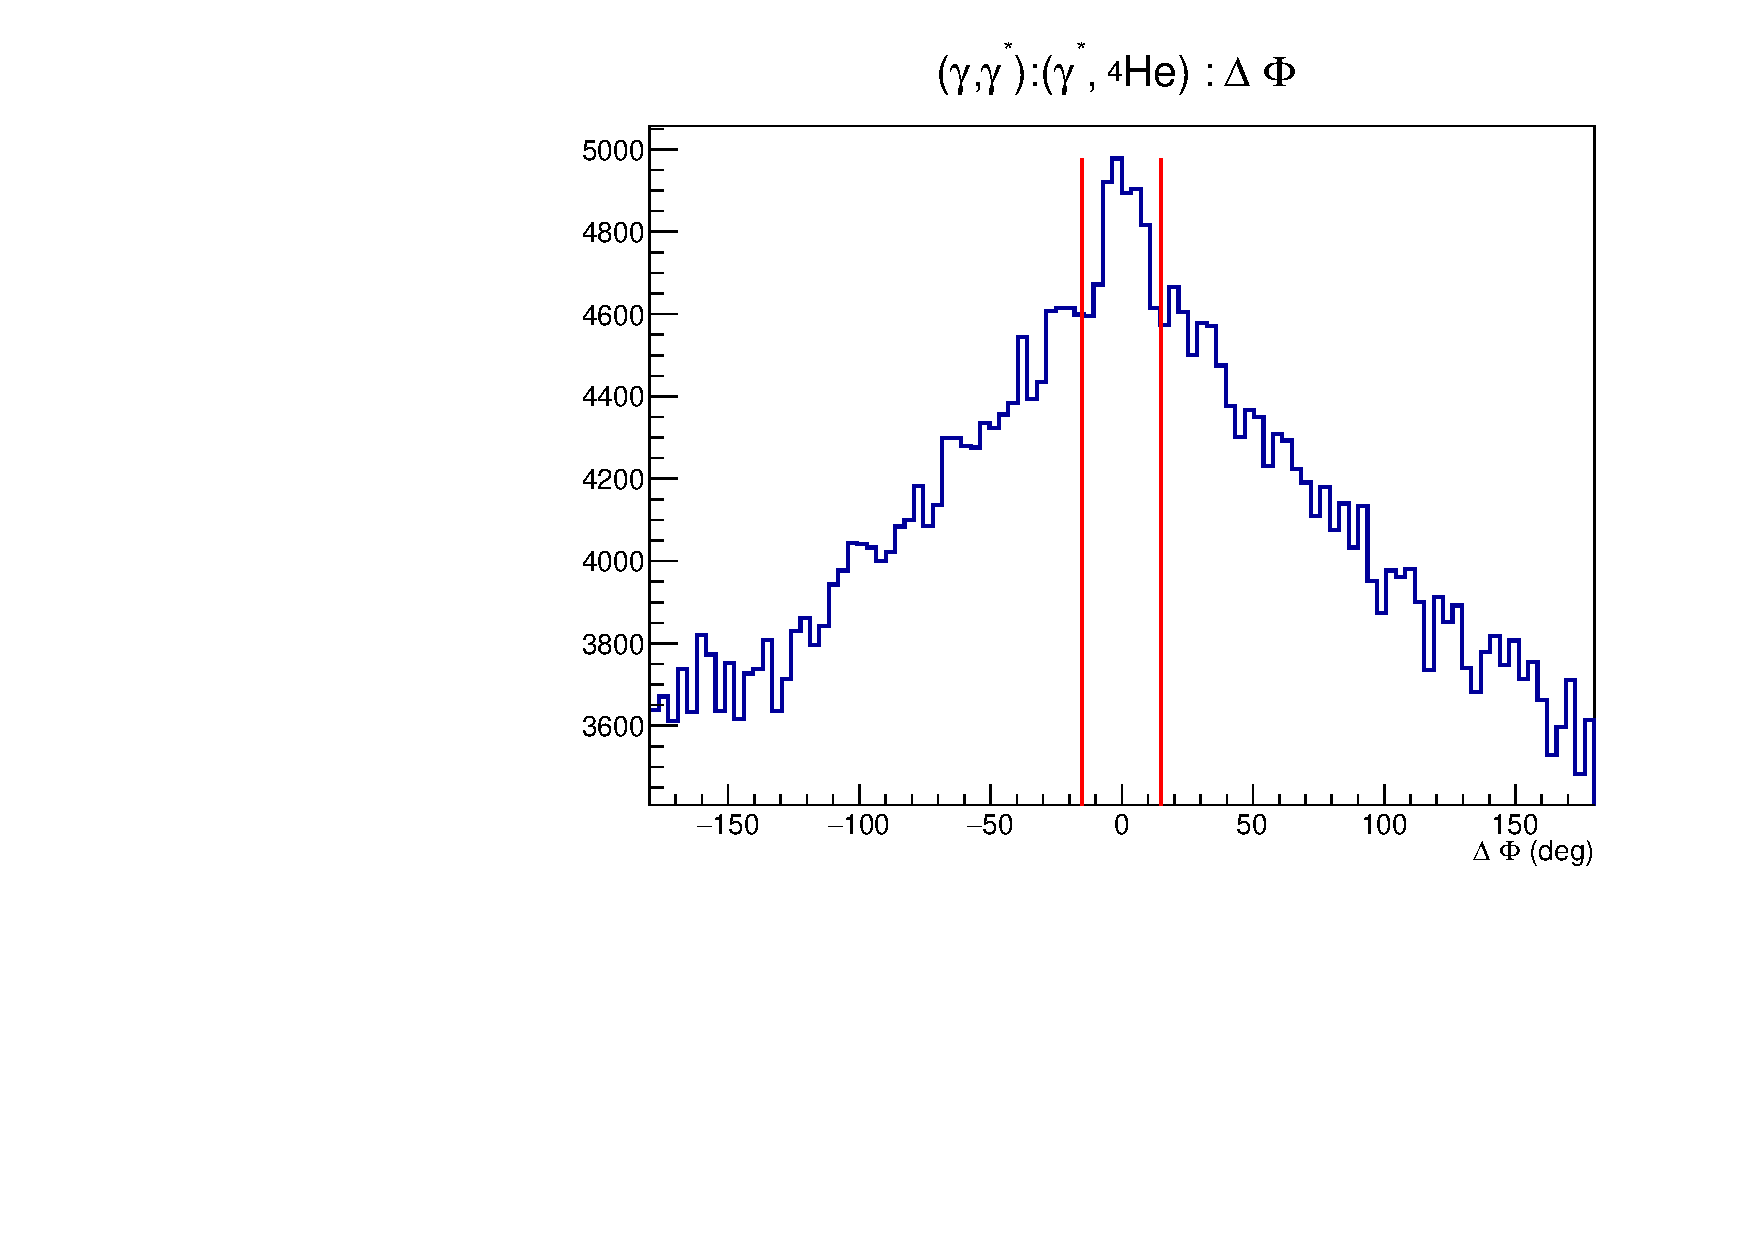
\includegraphics[width=\linewidth]{figures/dvcs_exclusivity_delta_phi.pdf}
    \end{minipage}
    \begin{minipage}{0.3\linewidth}
        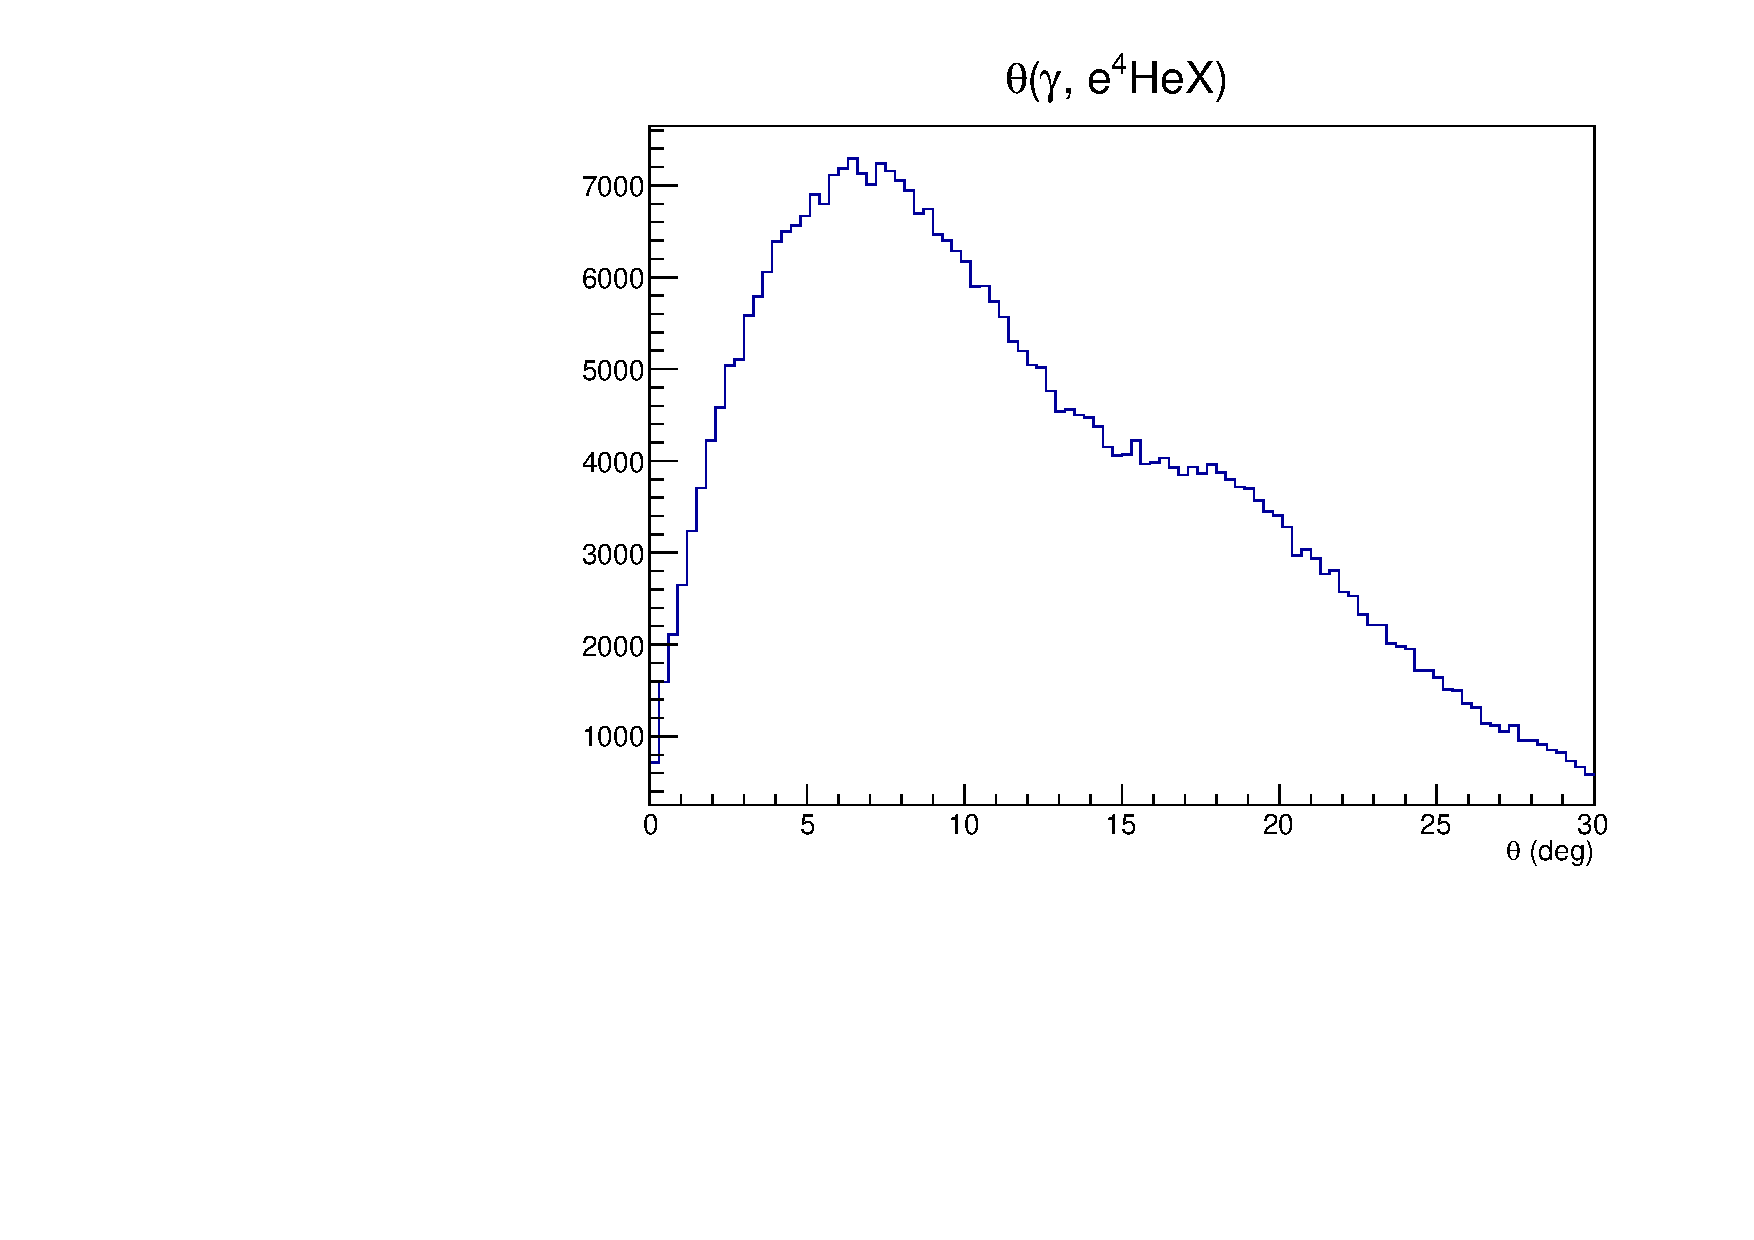
\includegraphics[width=\linewidth]{figures/dvcs_cone_angle_raw.pdf}
    \end{minipage}
    \begin{minipage}{0.3\linewidth}
        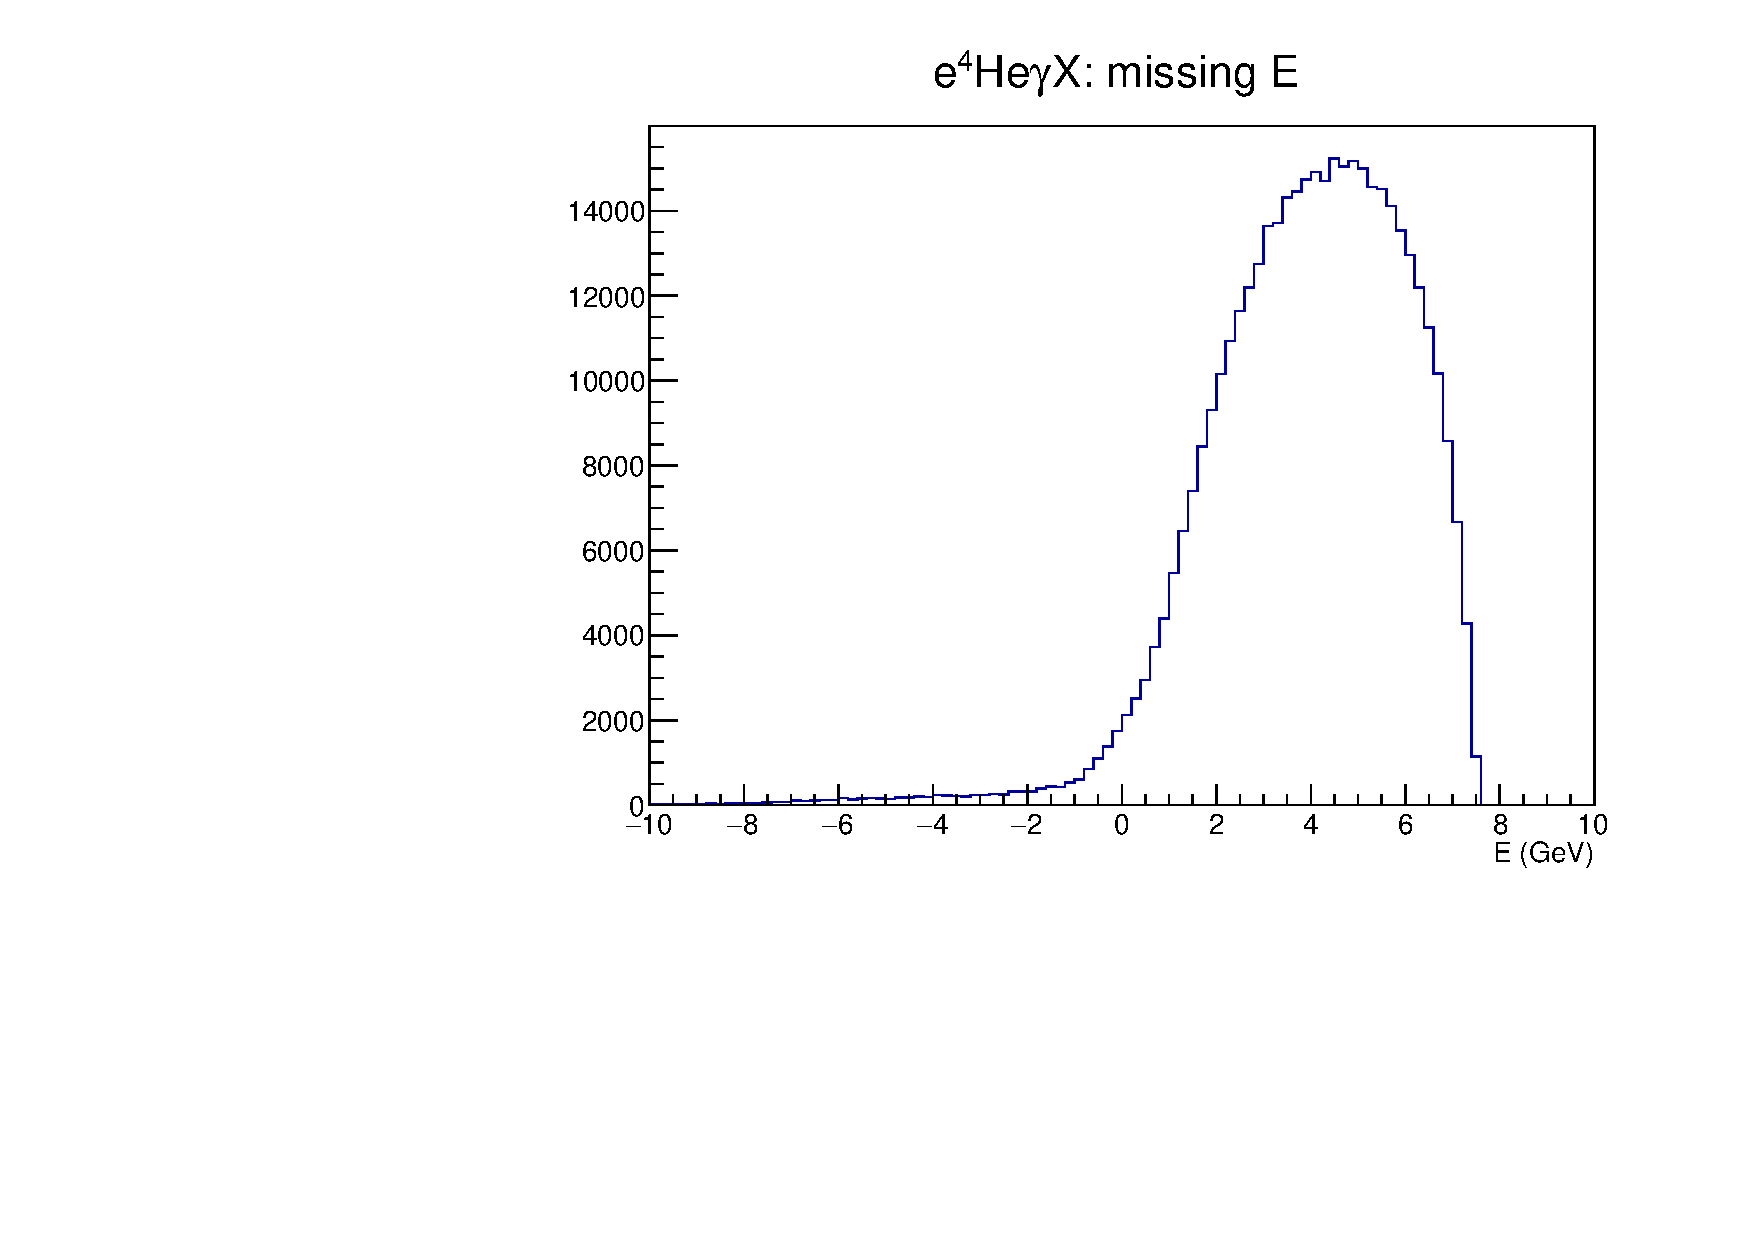
\includegraphics[width=\linewidth]{figures/dvcs_e4HegX_missing_E_raw.pdf}
    \end{minipage}
    \begin{minipage}{0.3\linewidth}
        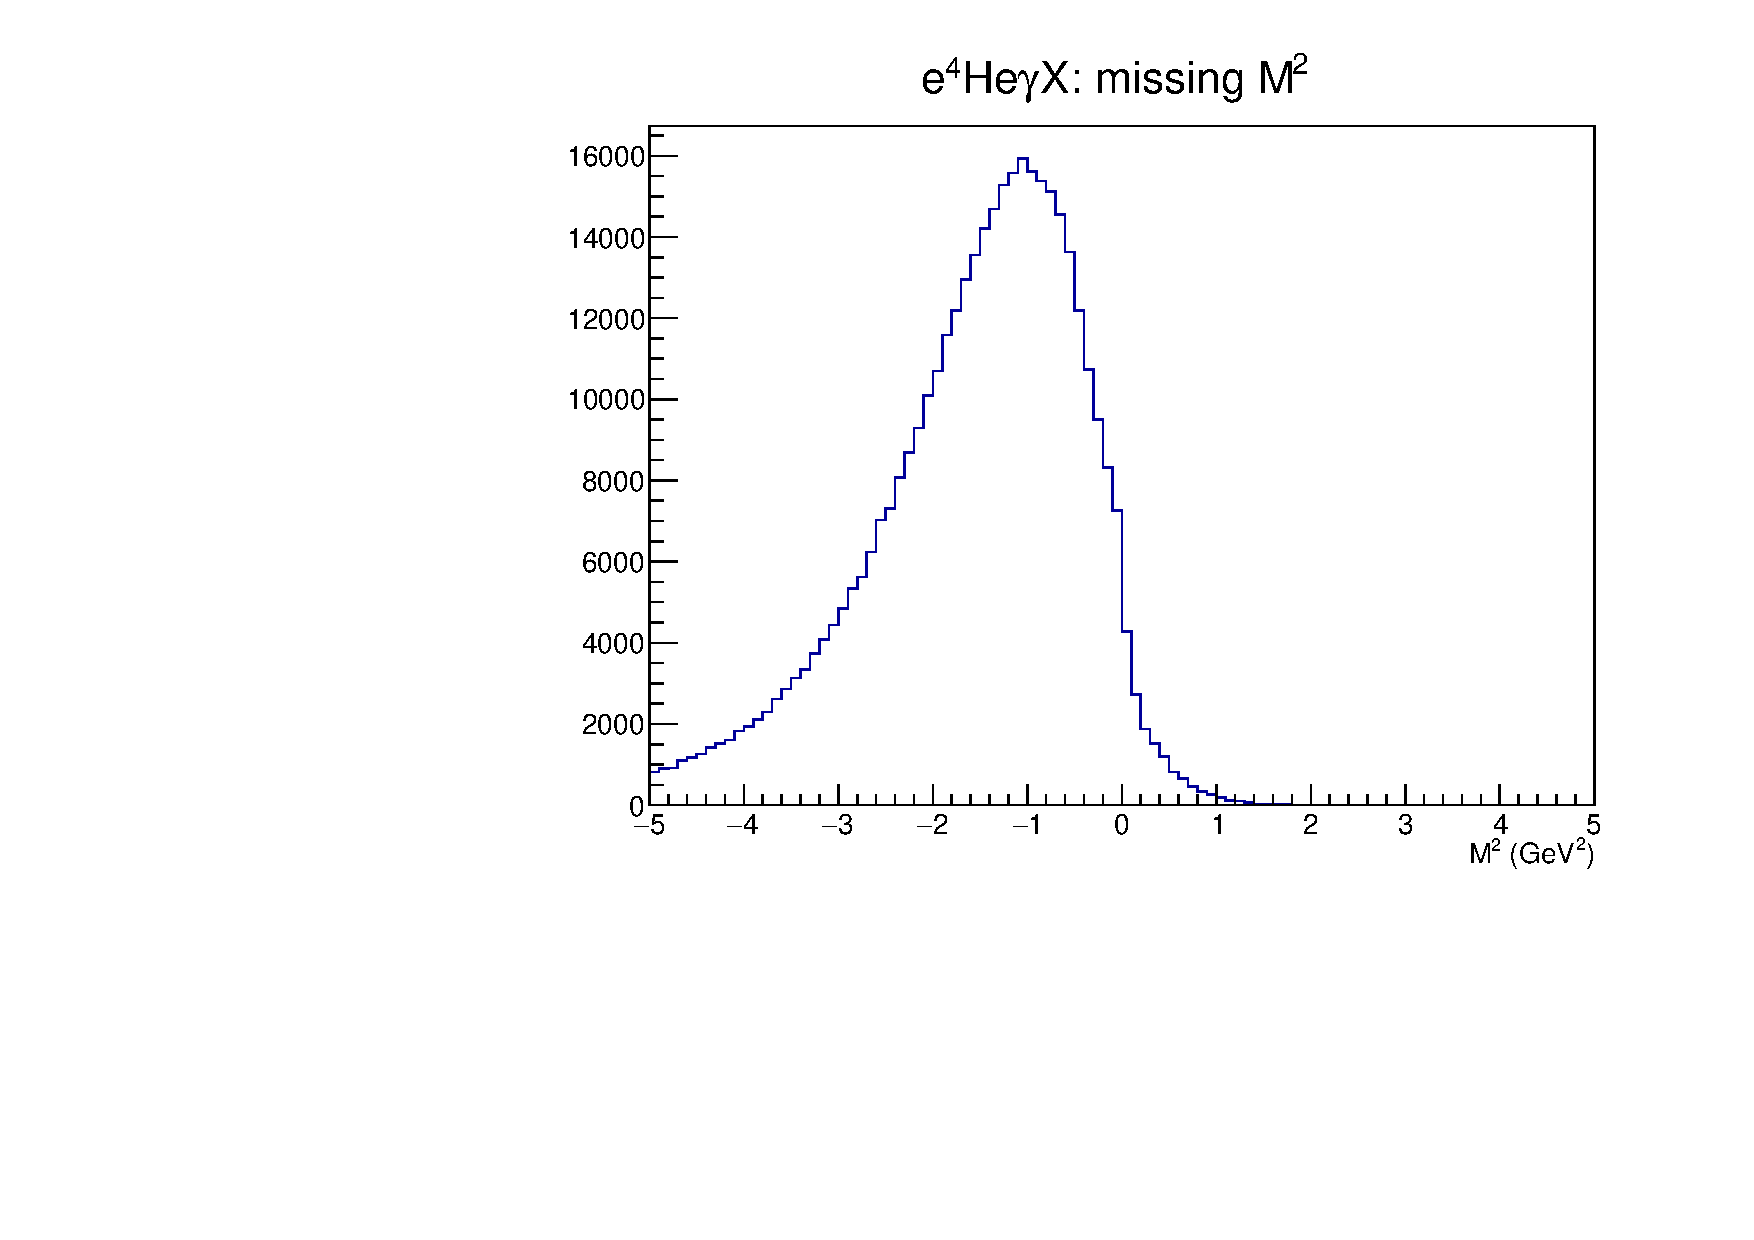
\includegraphics[width=\linewidth]{figures/dvcs_e4HegX_missing_M2_raw.pdf}
    \end{minipage}
    \begin{minipage}{0.3\linewidth}
        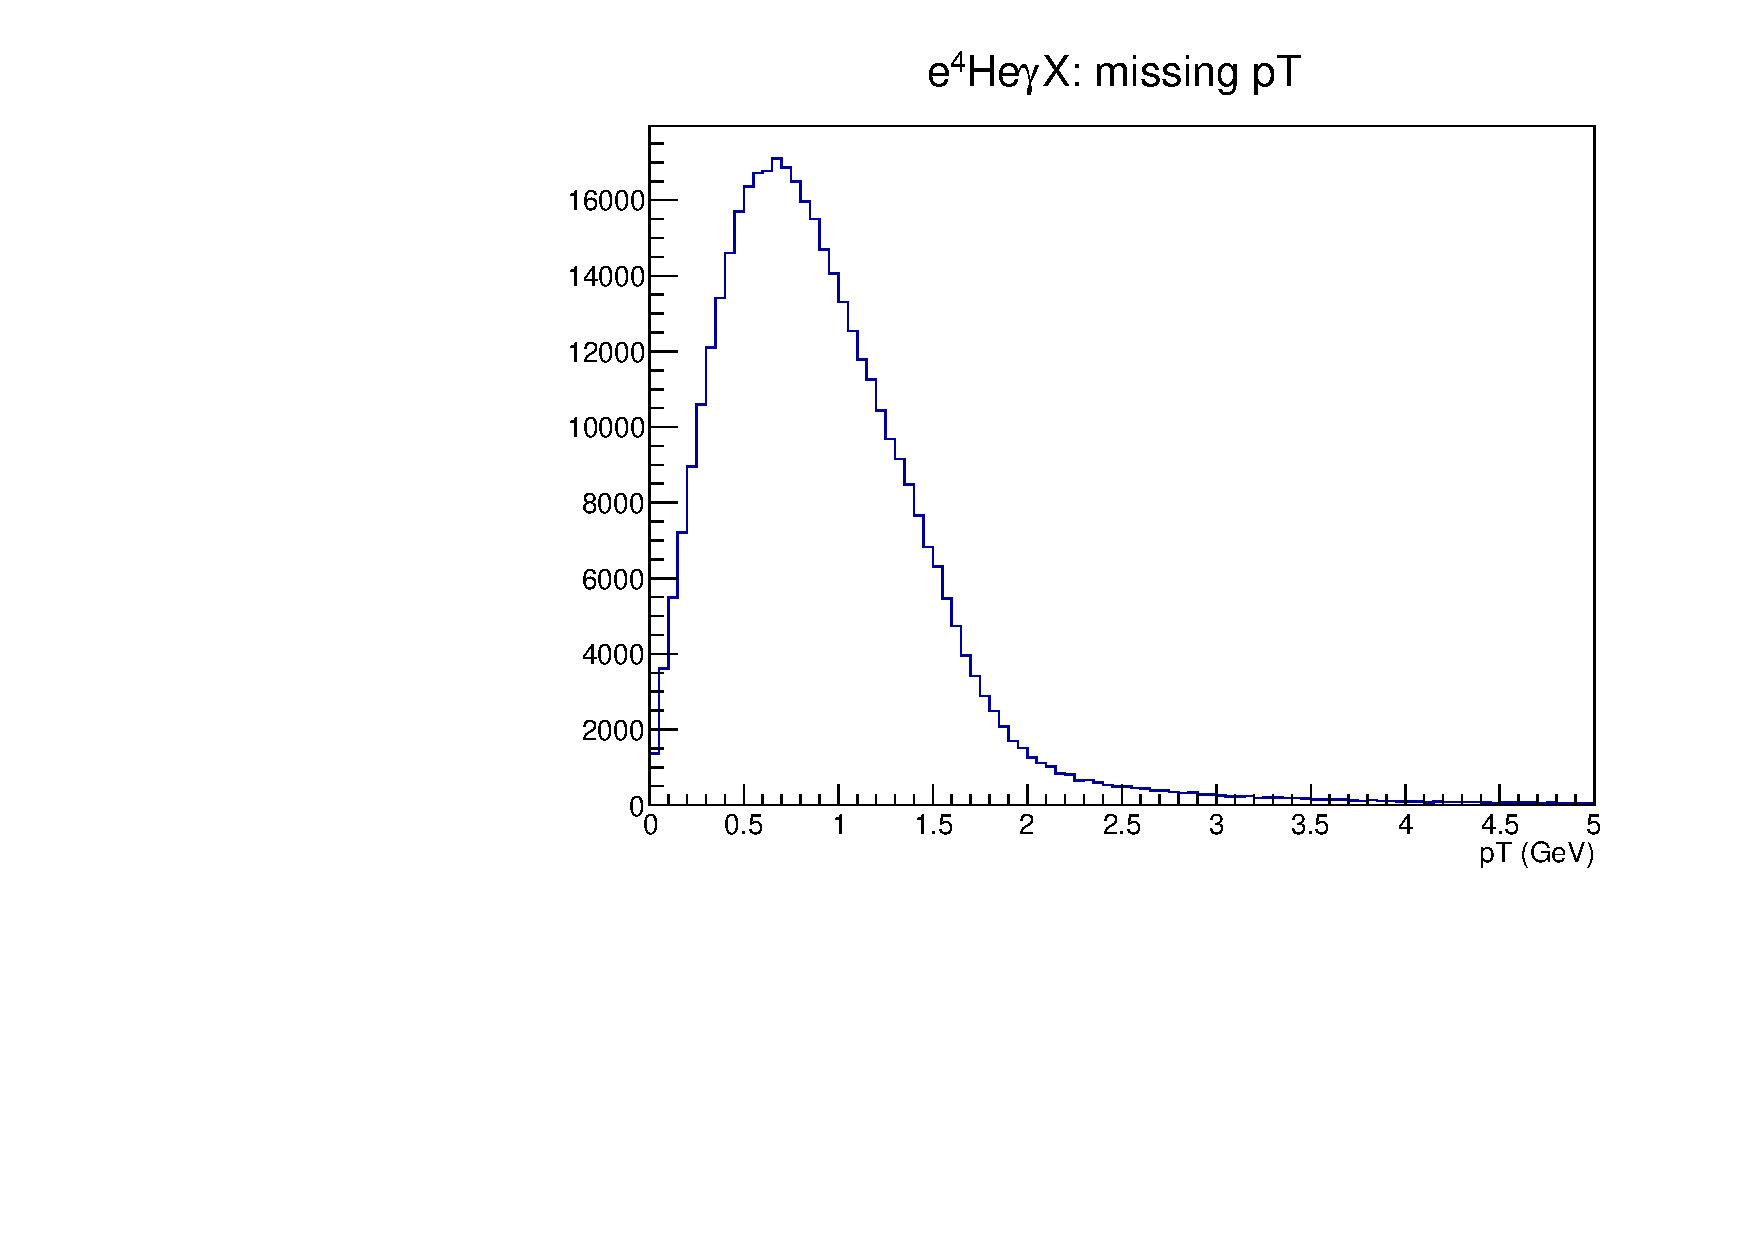
\includegraphics[width=\linewidth]{figures/dvcs_e4HegX_missing_pT_raw.pdf}
    \end{minipage}
    \begin{minipage}{0.3\linewidth}
        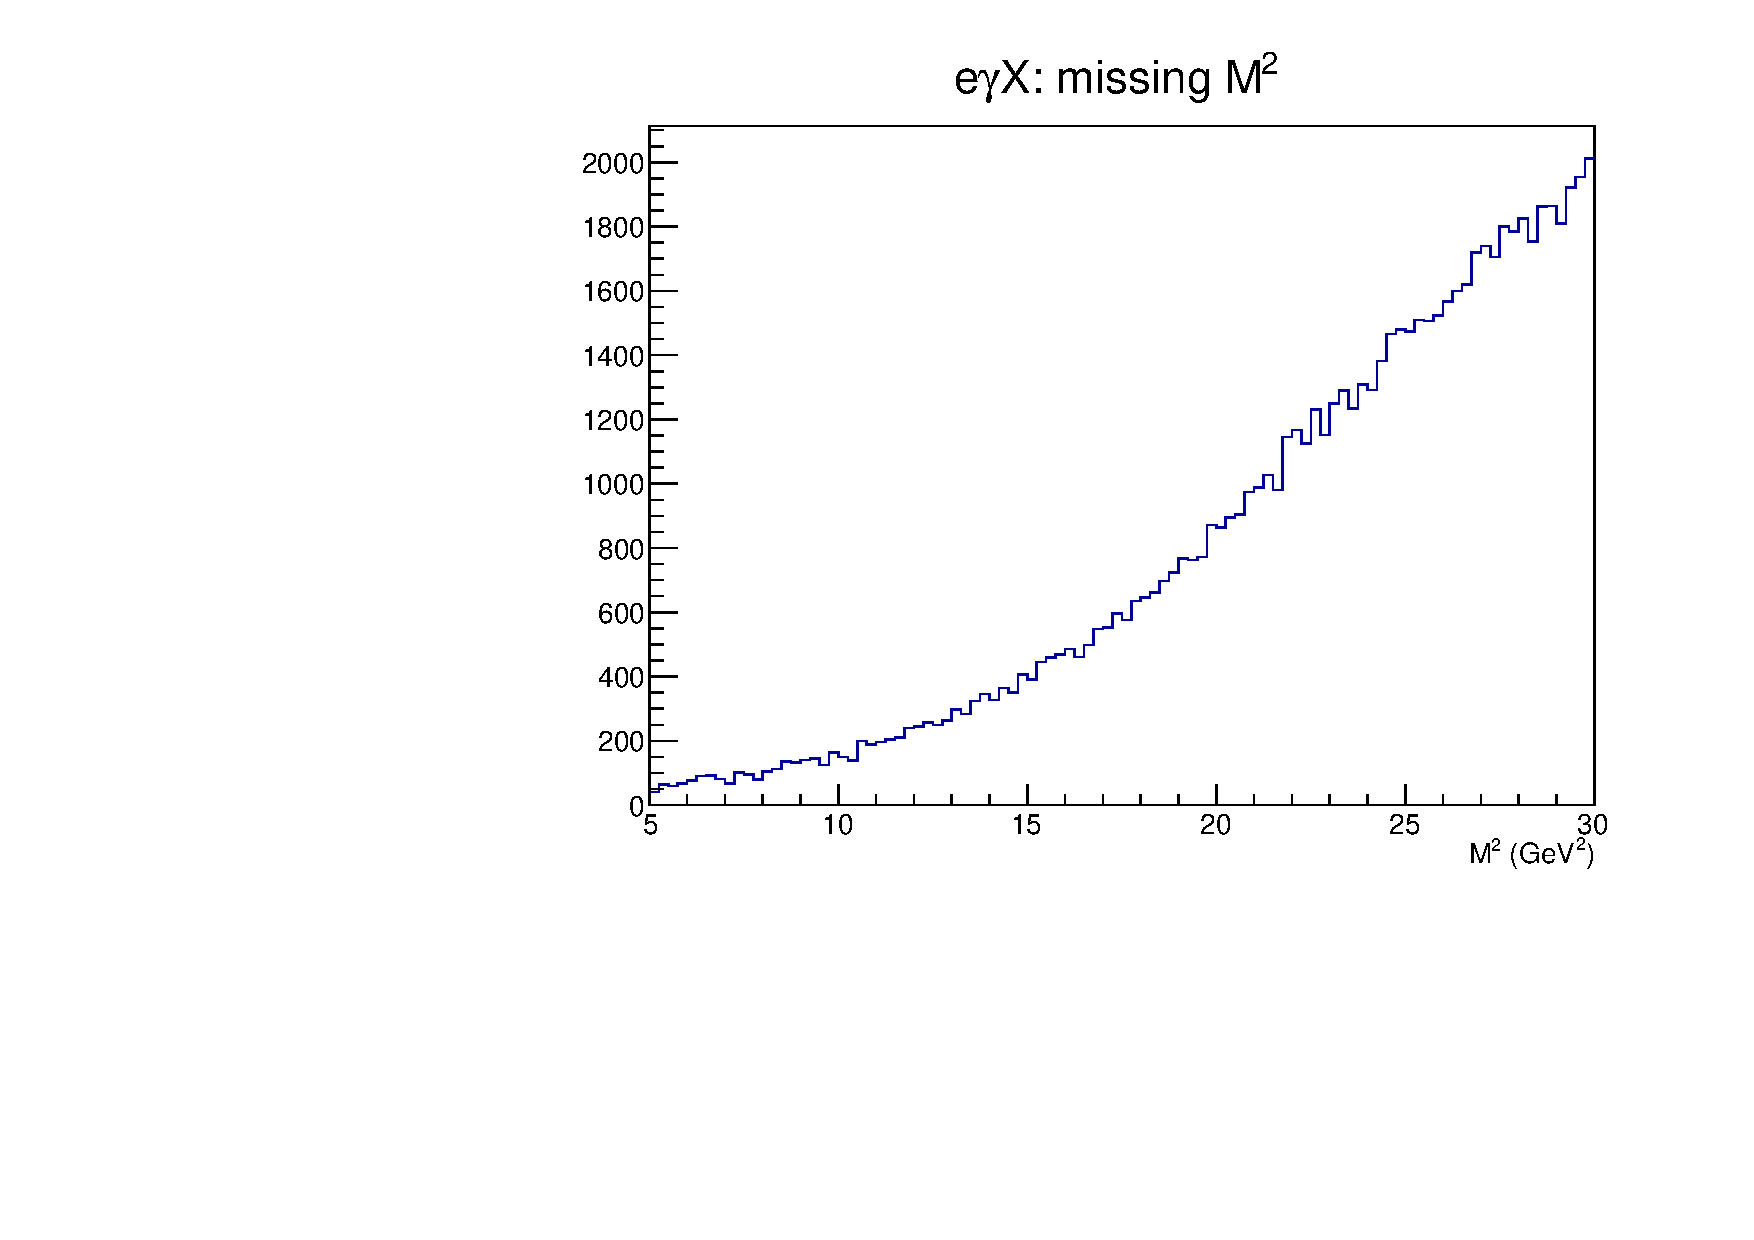
\includegraphics[width=\linewidth]{figures/dvcs_egX_missing_M2_raw.pdf}
    \end{minipage}

\end{frame}


\begin{frame}{DVCS candidates after $\Delta \Phi$ cut}
    \begin{itemize}
        \item After the cut on $\Delta \Phi$, others peaks appear
        \item The others cuts are : 
    \end{itemize}

    \centering
    \begin{minipage}{0.4\linewidth}
        \begin{itemize}
            \item[{\color{blue} $\circ$}] cone angle $< 2^{\circ}$
            \item[{\color{blue} $\circ$}] $e^4\mbox{He}gX.\mbox{M2} < 0.05 \mbox{ GeV}^2$ 
        \end{itemize}
    \end{minipage}
    \begin{minipage}{0.4\linewidth}
        \begin{itemize}
            \item[{\color{blue} $\circ$}] pT $<$ 0.25 GeV
            \item[{\color{blue} $\circ$}] $egX.\mbox{M2} < 20 \mbox{ GeV}^2$ 
        \end{itemize}
    \end{minipage}

    \centering
    \vspace{0.3cm}

    \begin{minipage}{0.3\linewidth}
        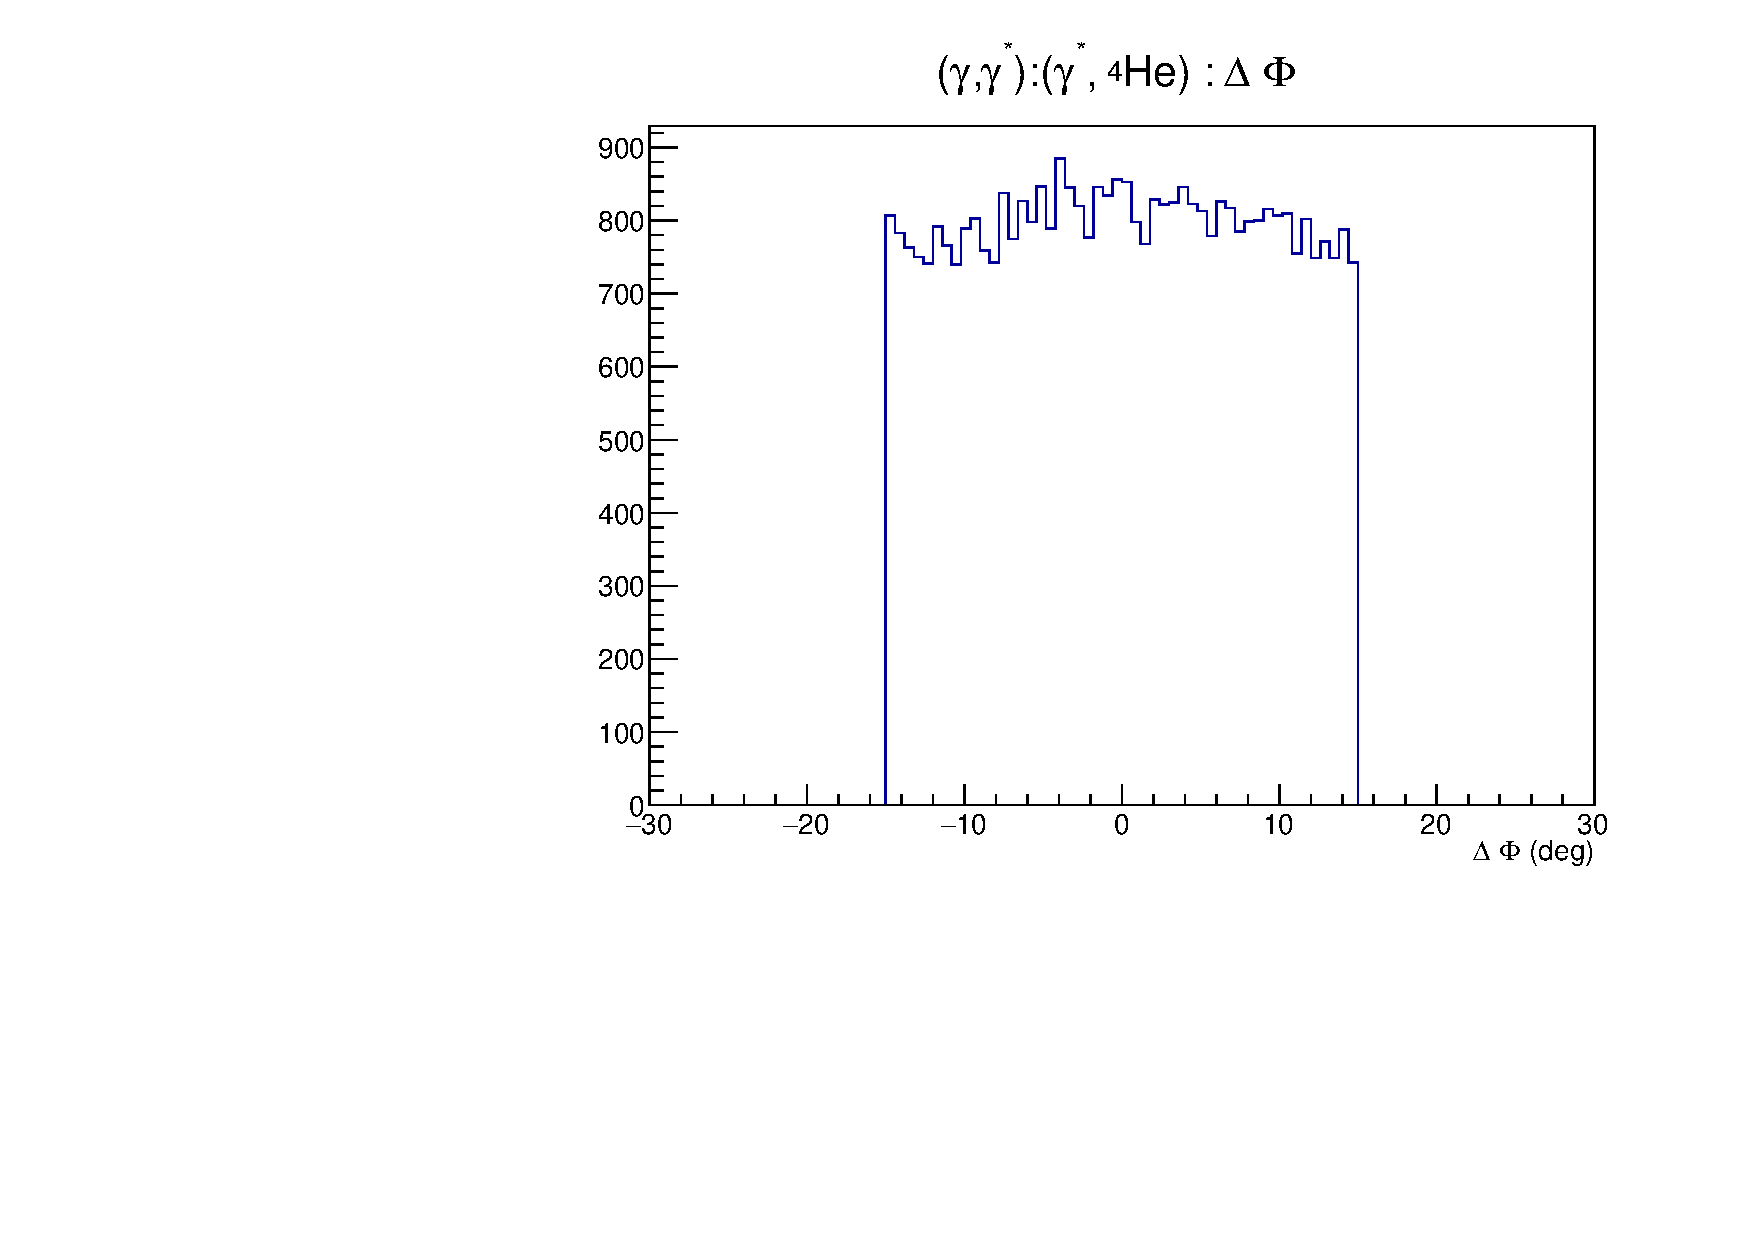
\includegraphics[width=\linewidth]{figures/dvcs_delta_phi_dphi_cut.pdf}
    \end{minipage}
    \begin{minipage}{0.3\linewidth}
        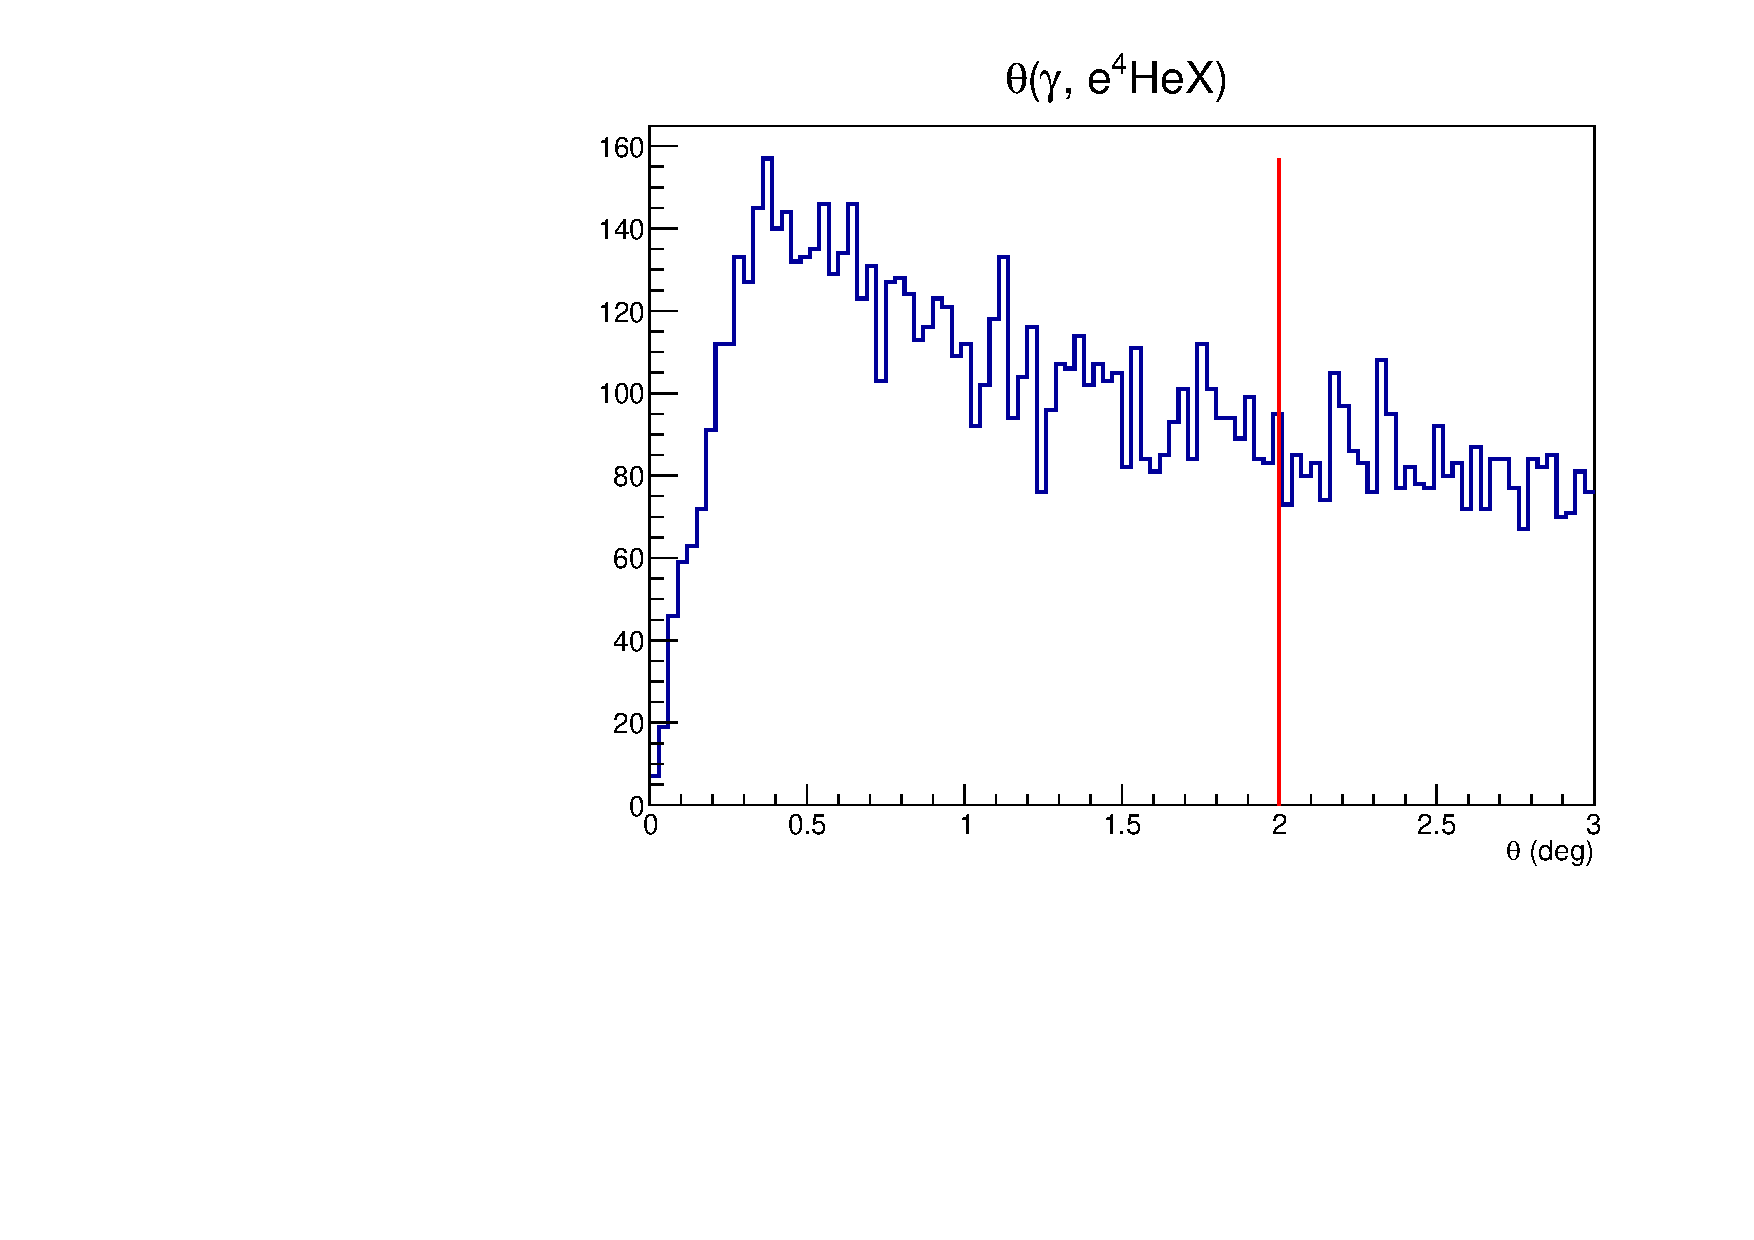
\includegraphics[width=\linewidth]{figures/dvcs_exclusivity_cone_angle.pdf}
    \end{minipage}
    \begin{minipage}{0.3\linewidth}
        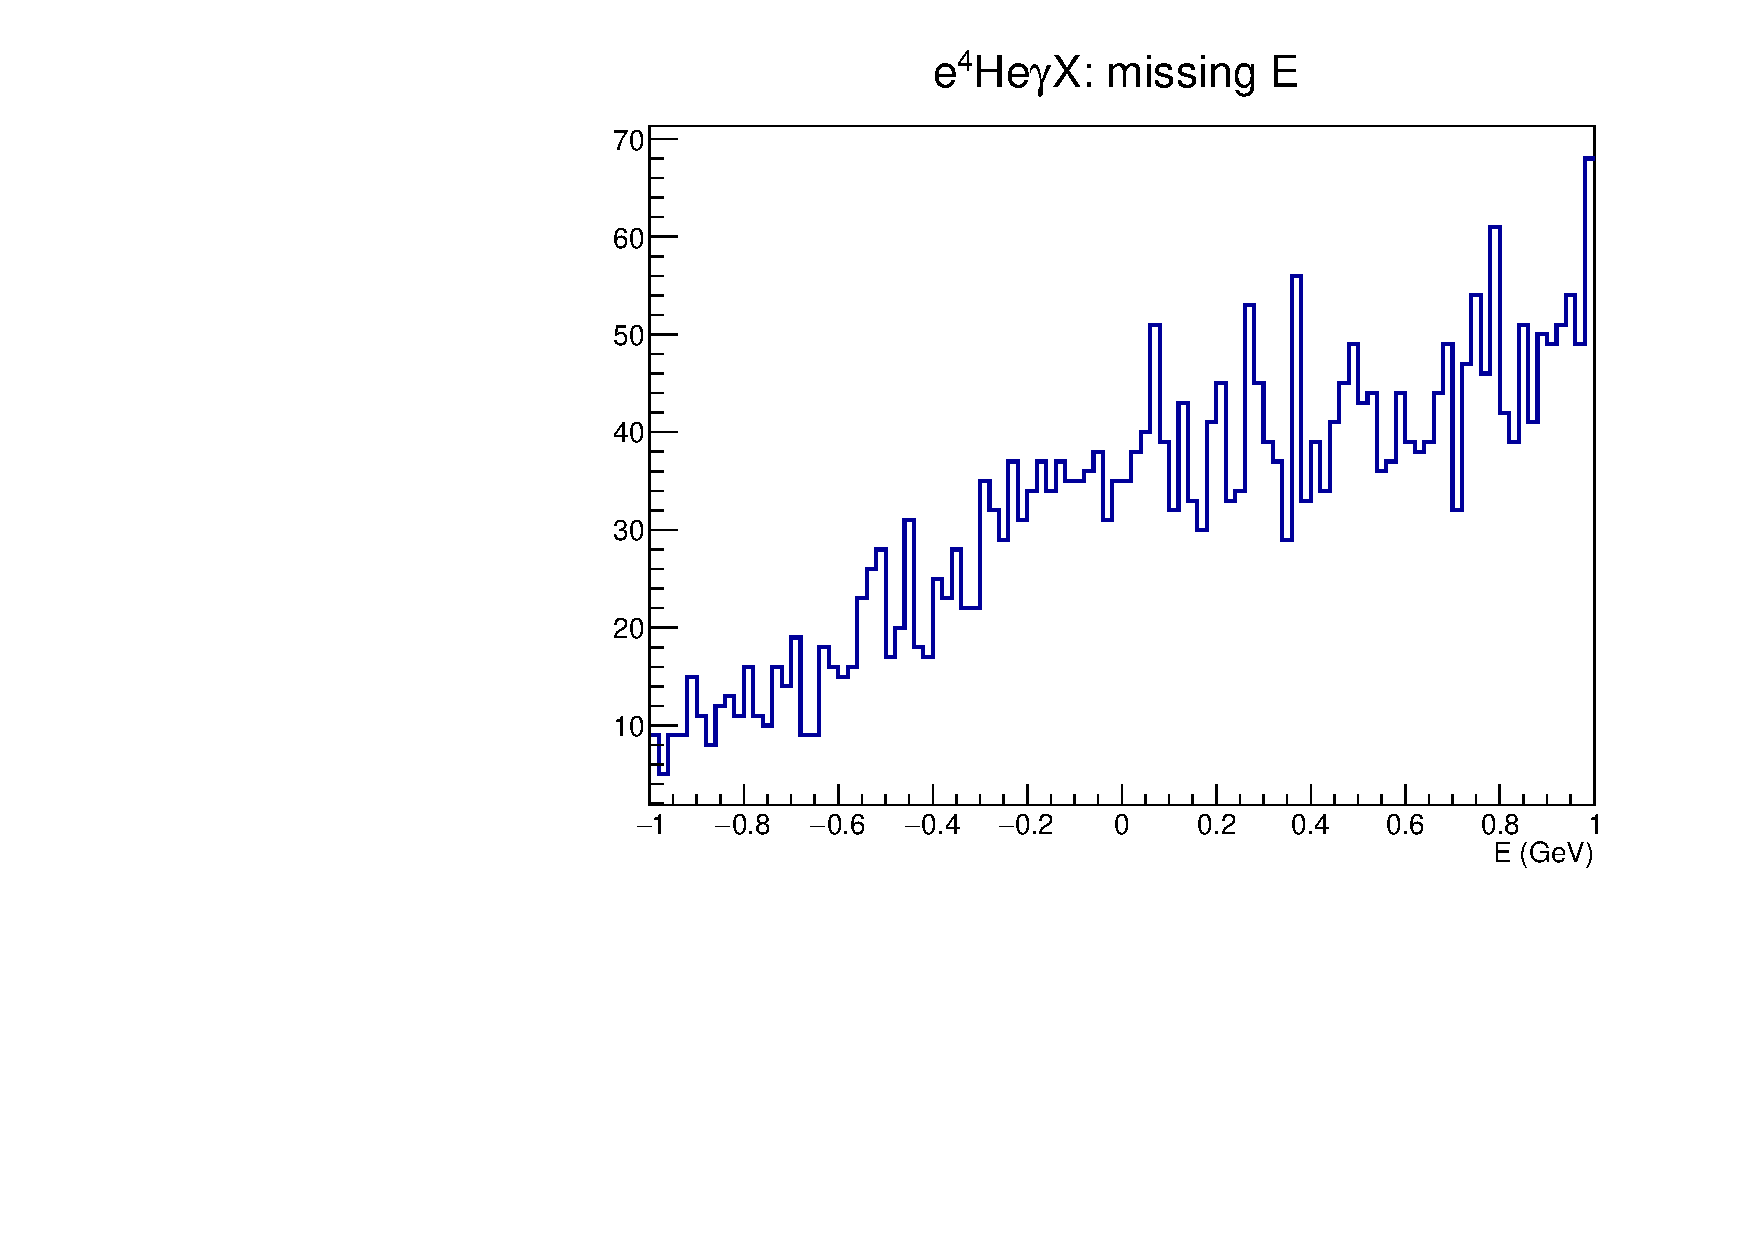
\includegraphics[width=\linewidth]{figures/dvcs_exclusivity_e4HegX_missing_E.pdf}
    \end{minipage}
    \begin{minipage}{0.3\linewidth}
        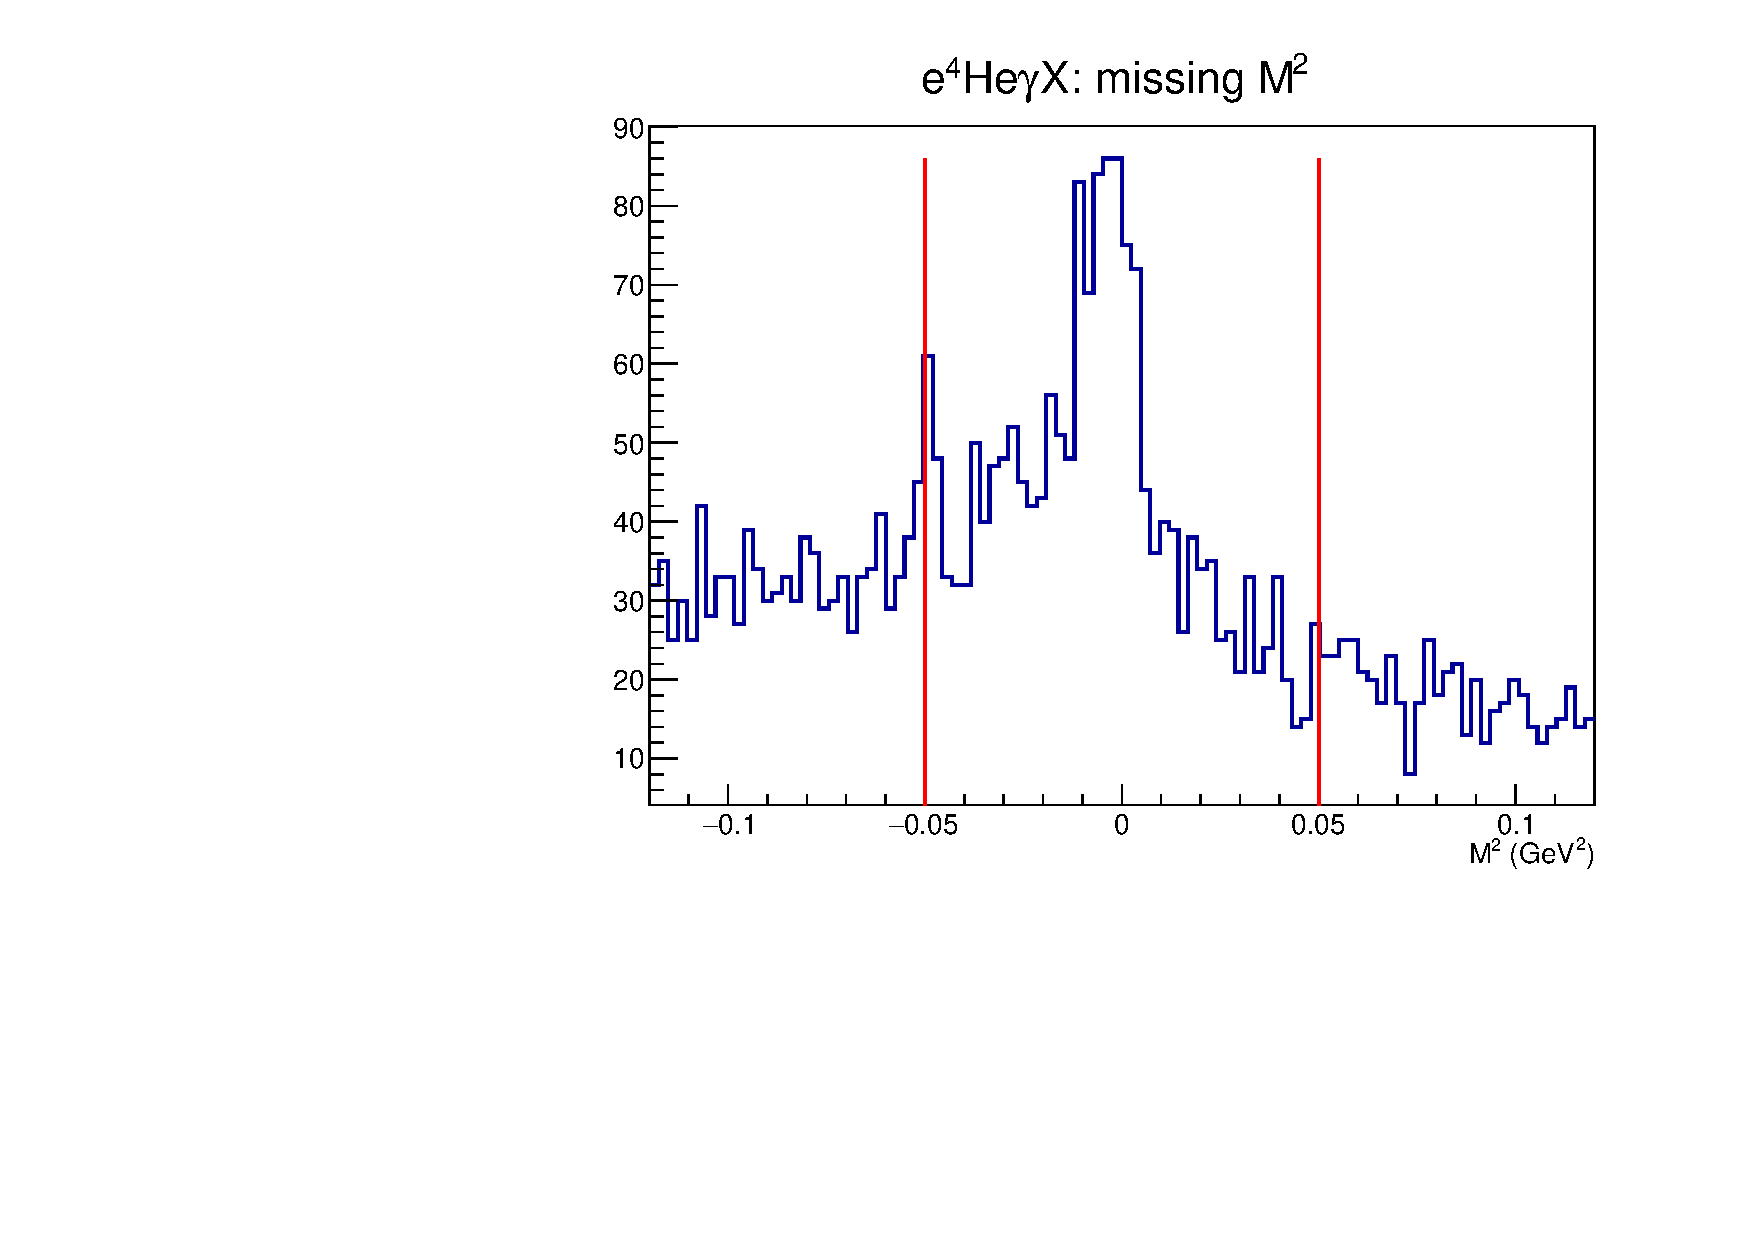
\includegraphics[width=\linewidth]{figures/dvcs_exclusivity_e4HegX_missing_M2.pdf}
    \end{minipage}
    \begin{minipage}{0.3\linewidth}
        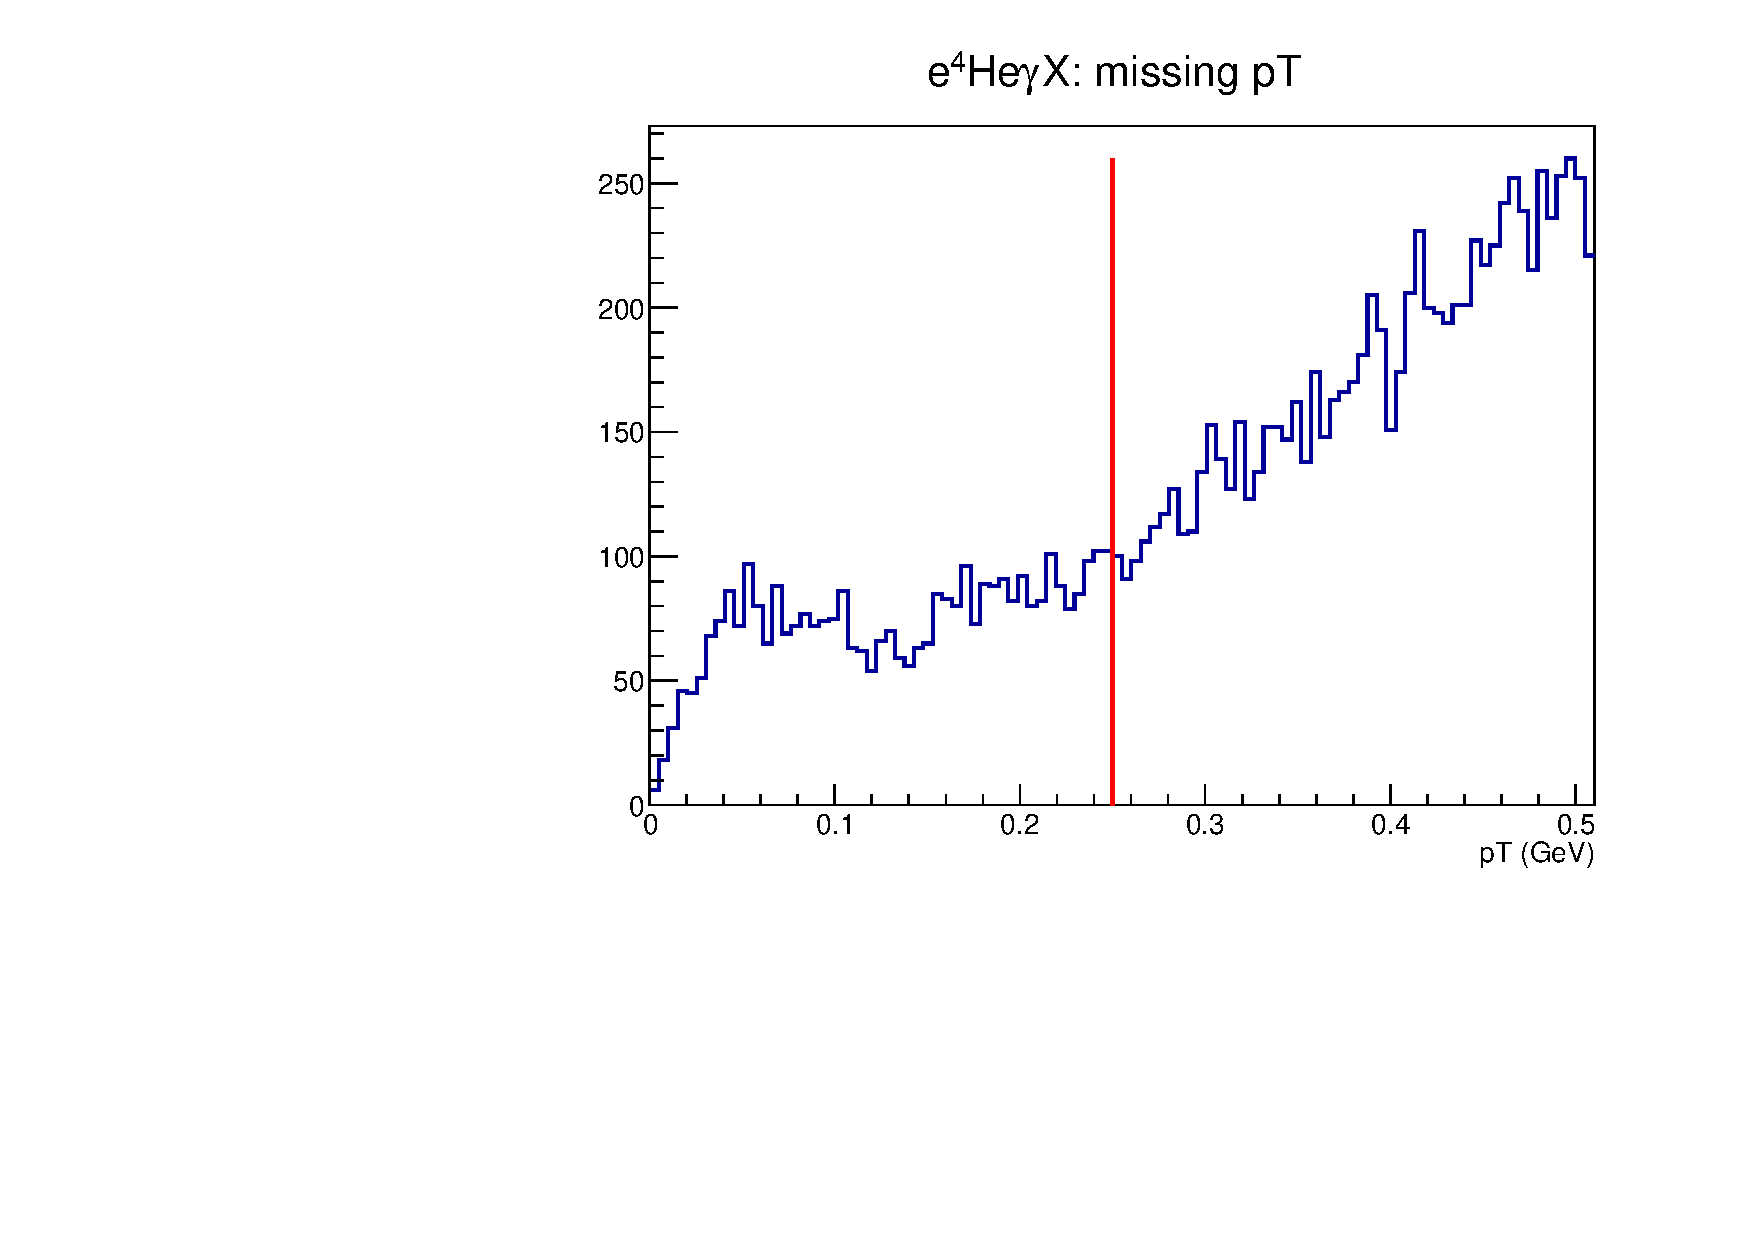
\includegraphics[width=\linewidth]{figures/dvcs_exclusivity_e4HegX_missing_pT.pdf}
    \end{minipage}
    \begin{minipage}{0.3\linewidth}
        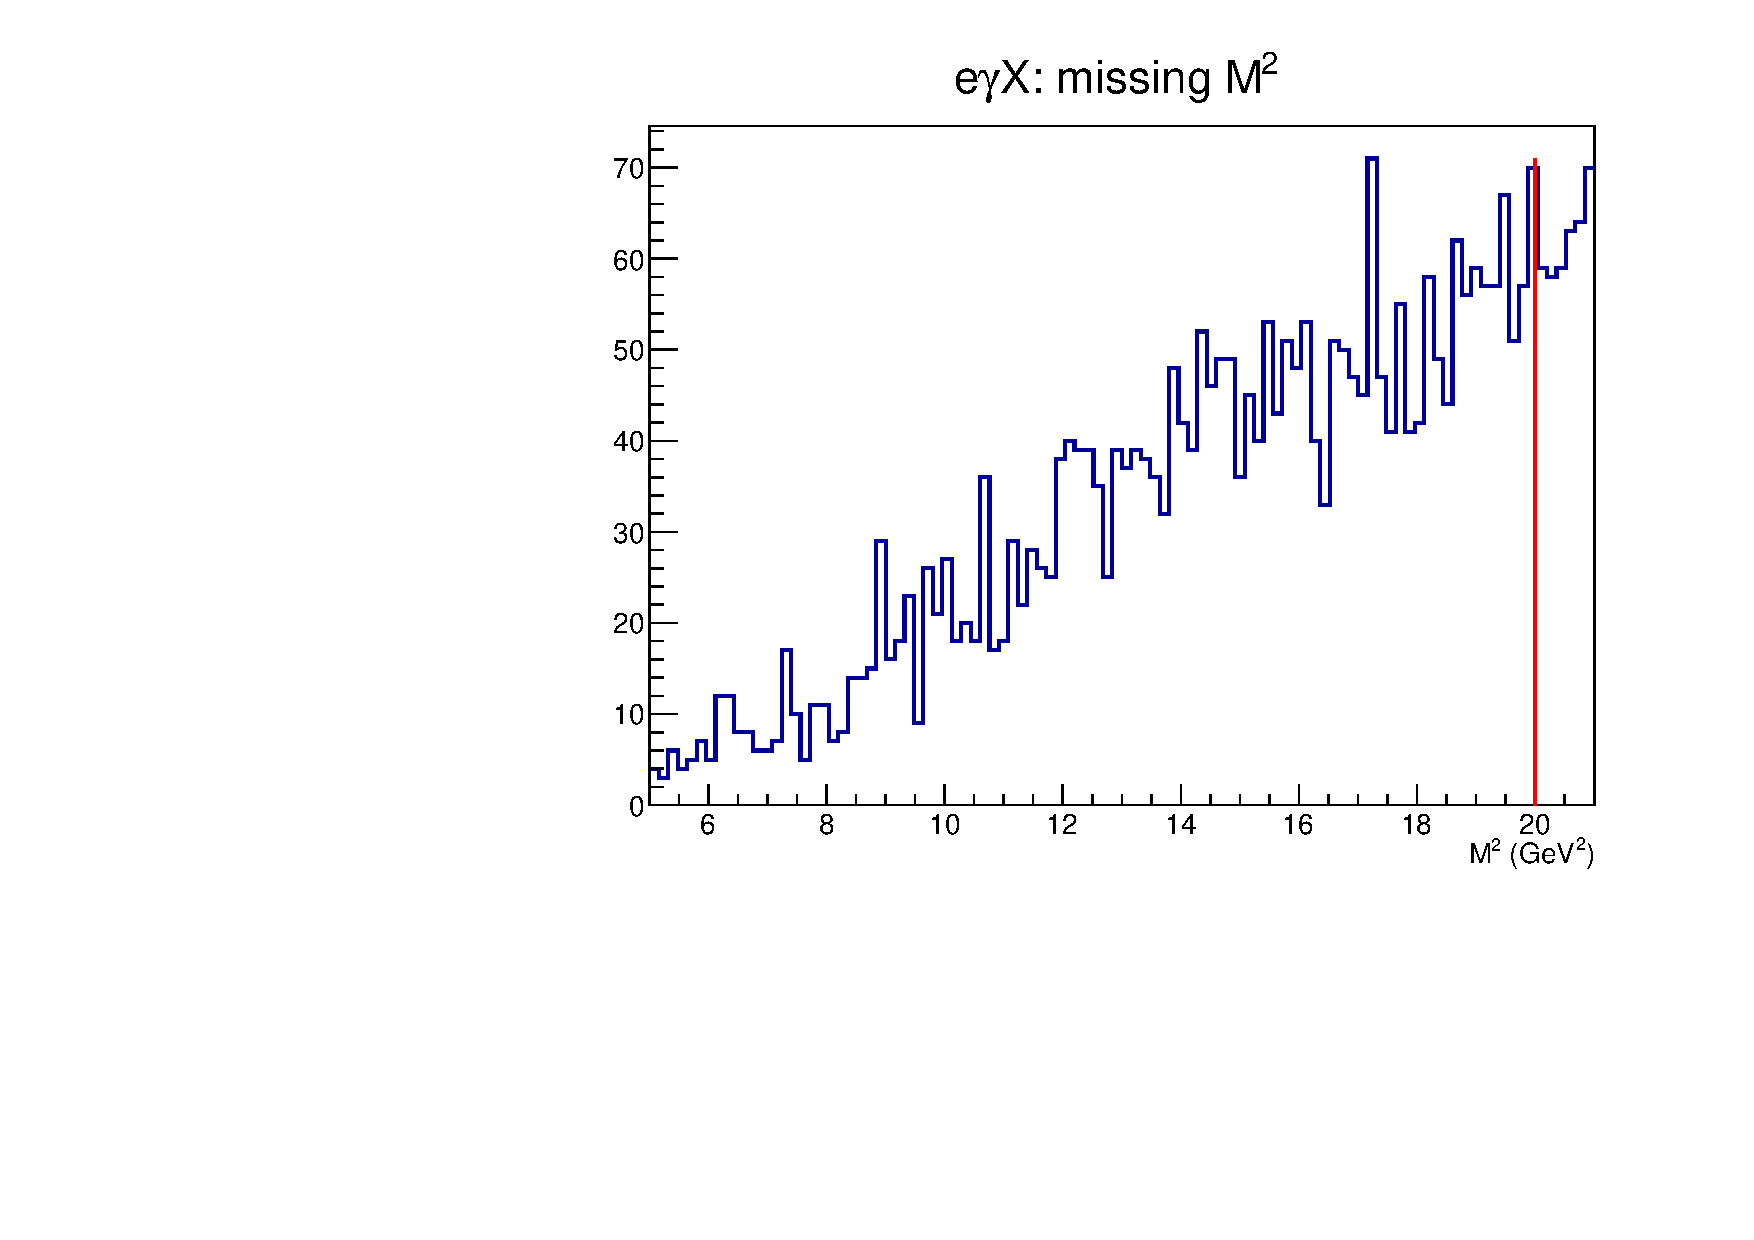
\includegraphics[width=\linewidth]{figures/dvcs_exclusivity_egX_missing_M2.pdf}
    \end{minipage}

\end{frame}

\begin{frame}{DVCS exclusivity cuts}

    \begin{itemize}
        \item Here are the distributions after all exclusivity cuts
        %\item We count 1038 DVCS events for only 7.53 \% of all $^4\mbox{He}$ data at 10.6 GeV
    \end{itemize}

    \centering
    \vspace{0.3cm}

    \begin{minipage}{0.3\linewidth}
        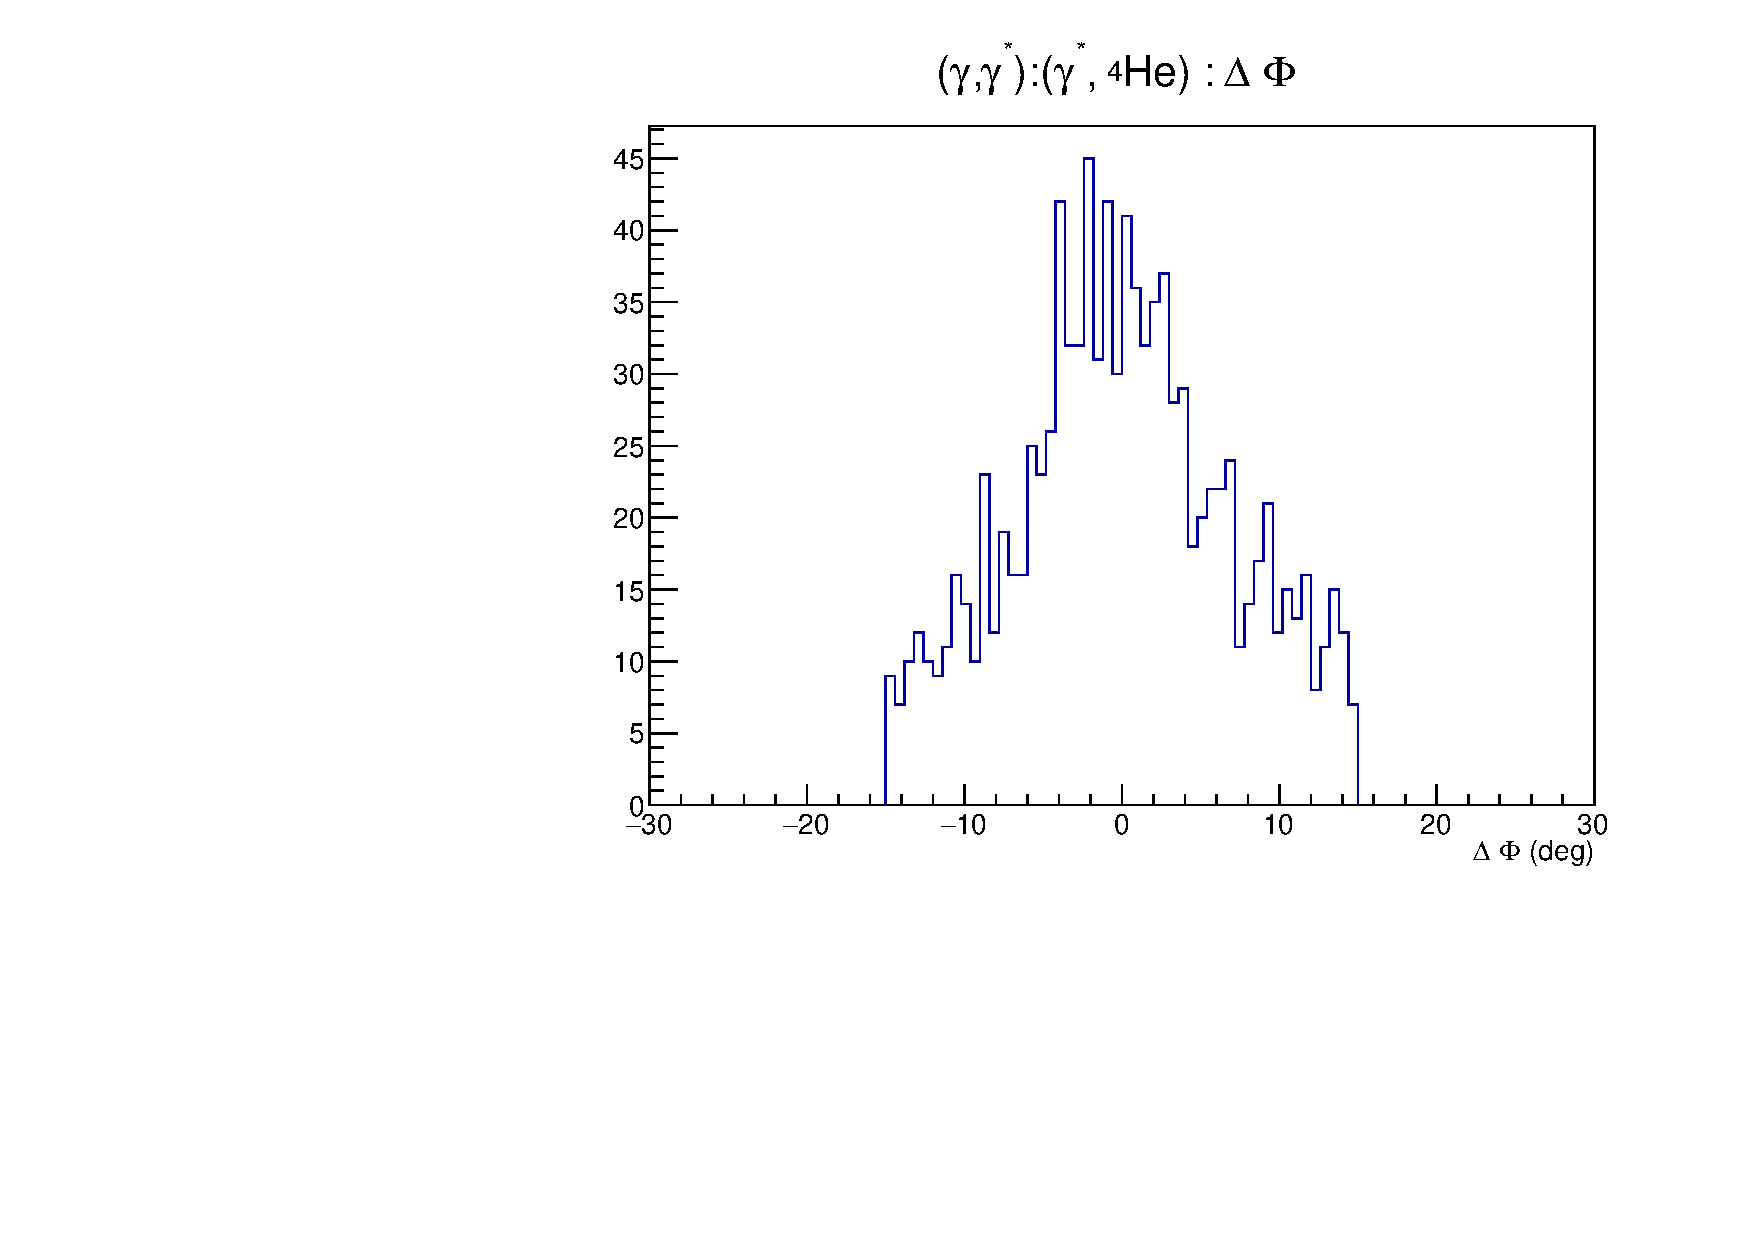
\includegraphics[width=\linewidth]{figures/dvcs_delta_phi.pdf}
    \end{minipage}
    \begin{minipage}{0.3\linewidth}
        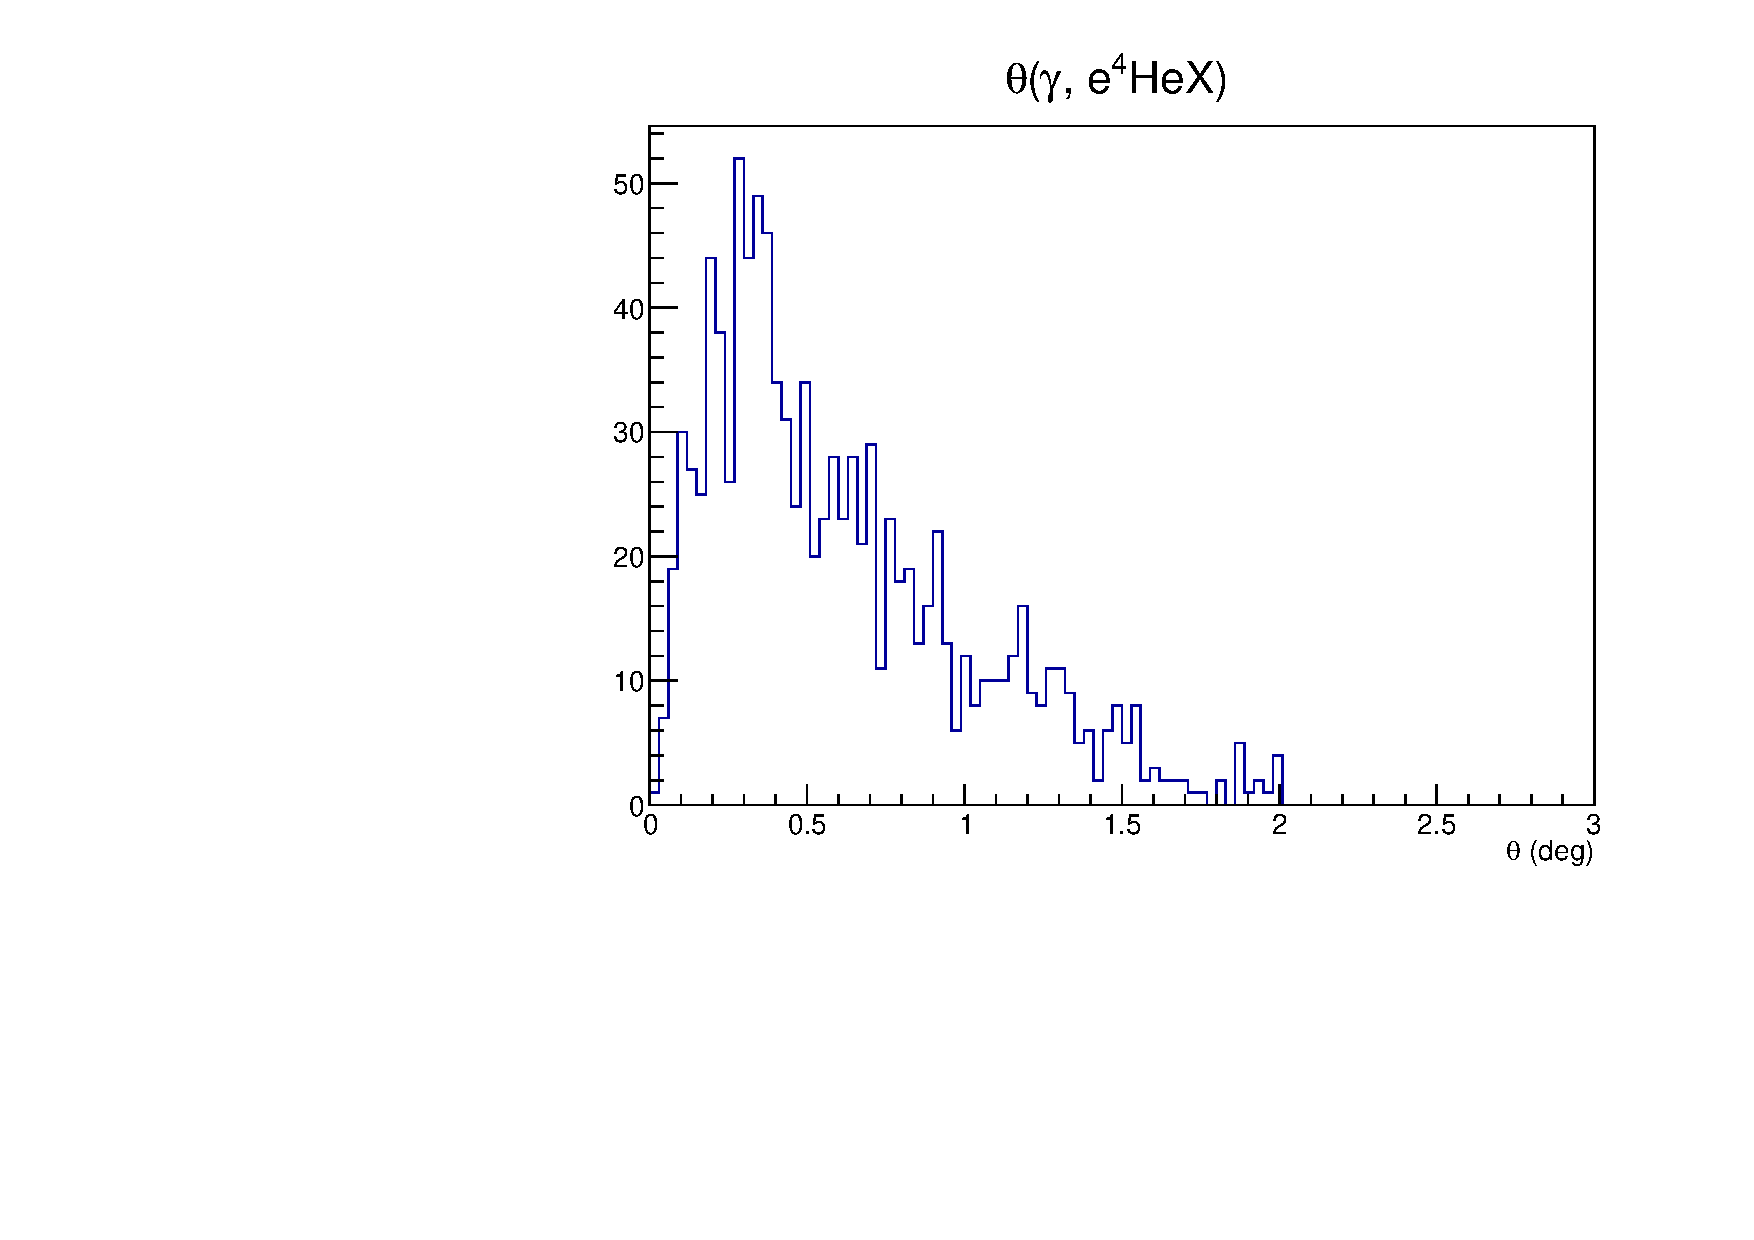
\includegraphics[width=\linewidth]{figures/dvcs_cone_angle.pdf}
    \end{minipage}
    \begin{minipage}{0.3\linewidth}
        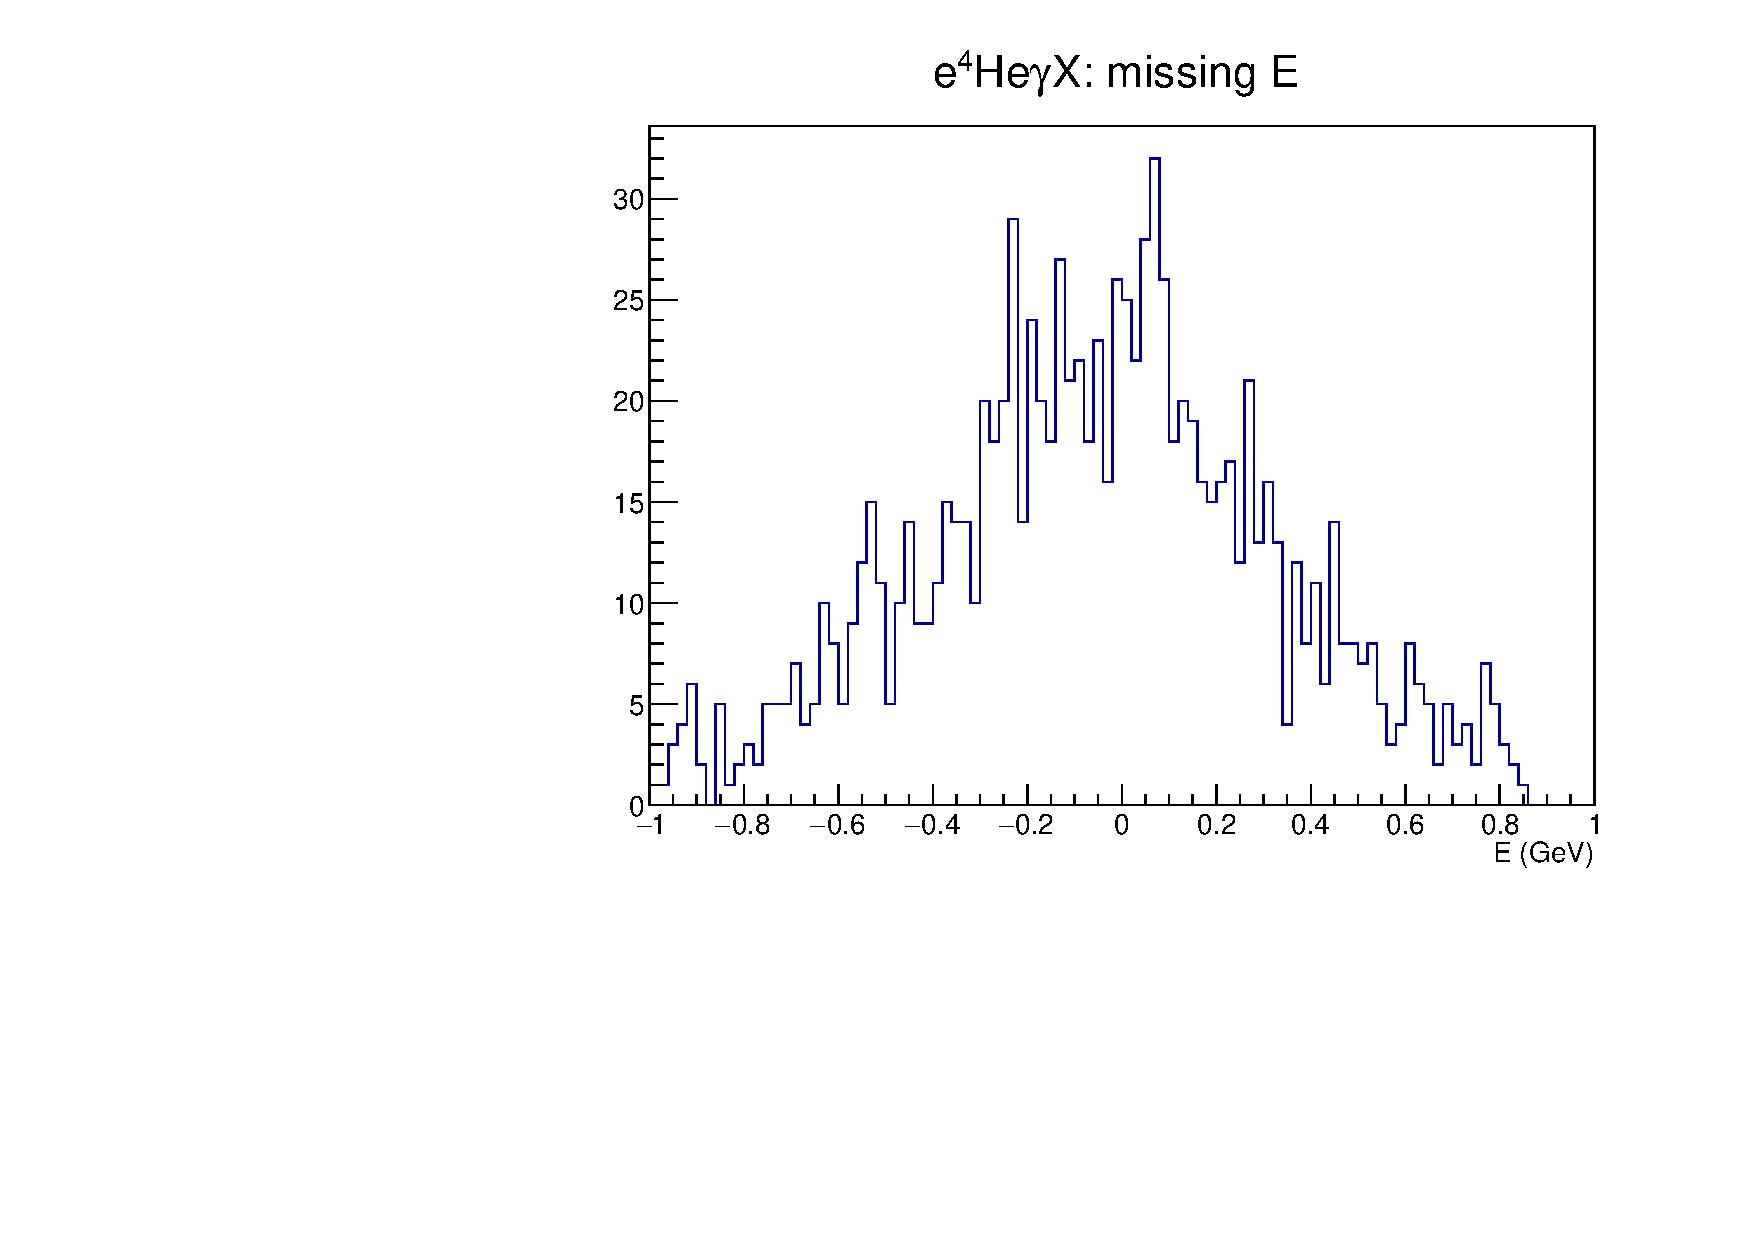
\includegraphics[width=\linewidth]{figures/dvcs_e4HegX_missing_E.pdf}
    \end{minipage}
    \begin{minipage}{0.3\linewidth}
        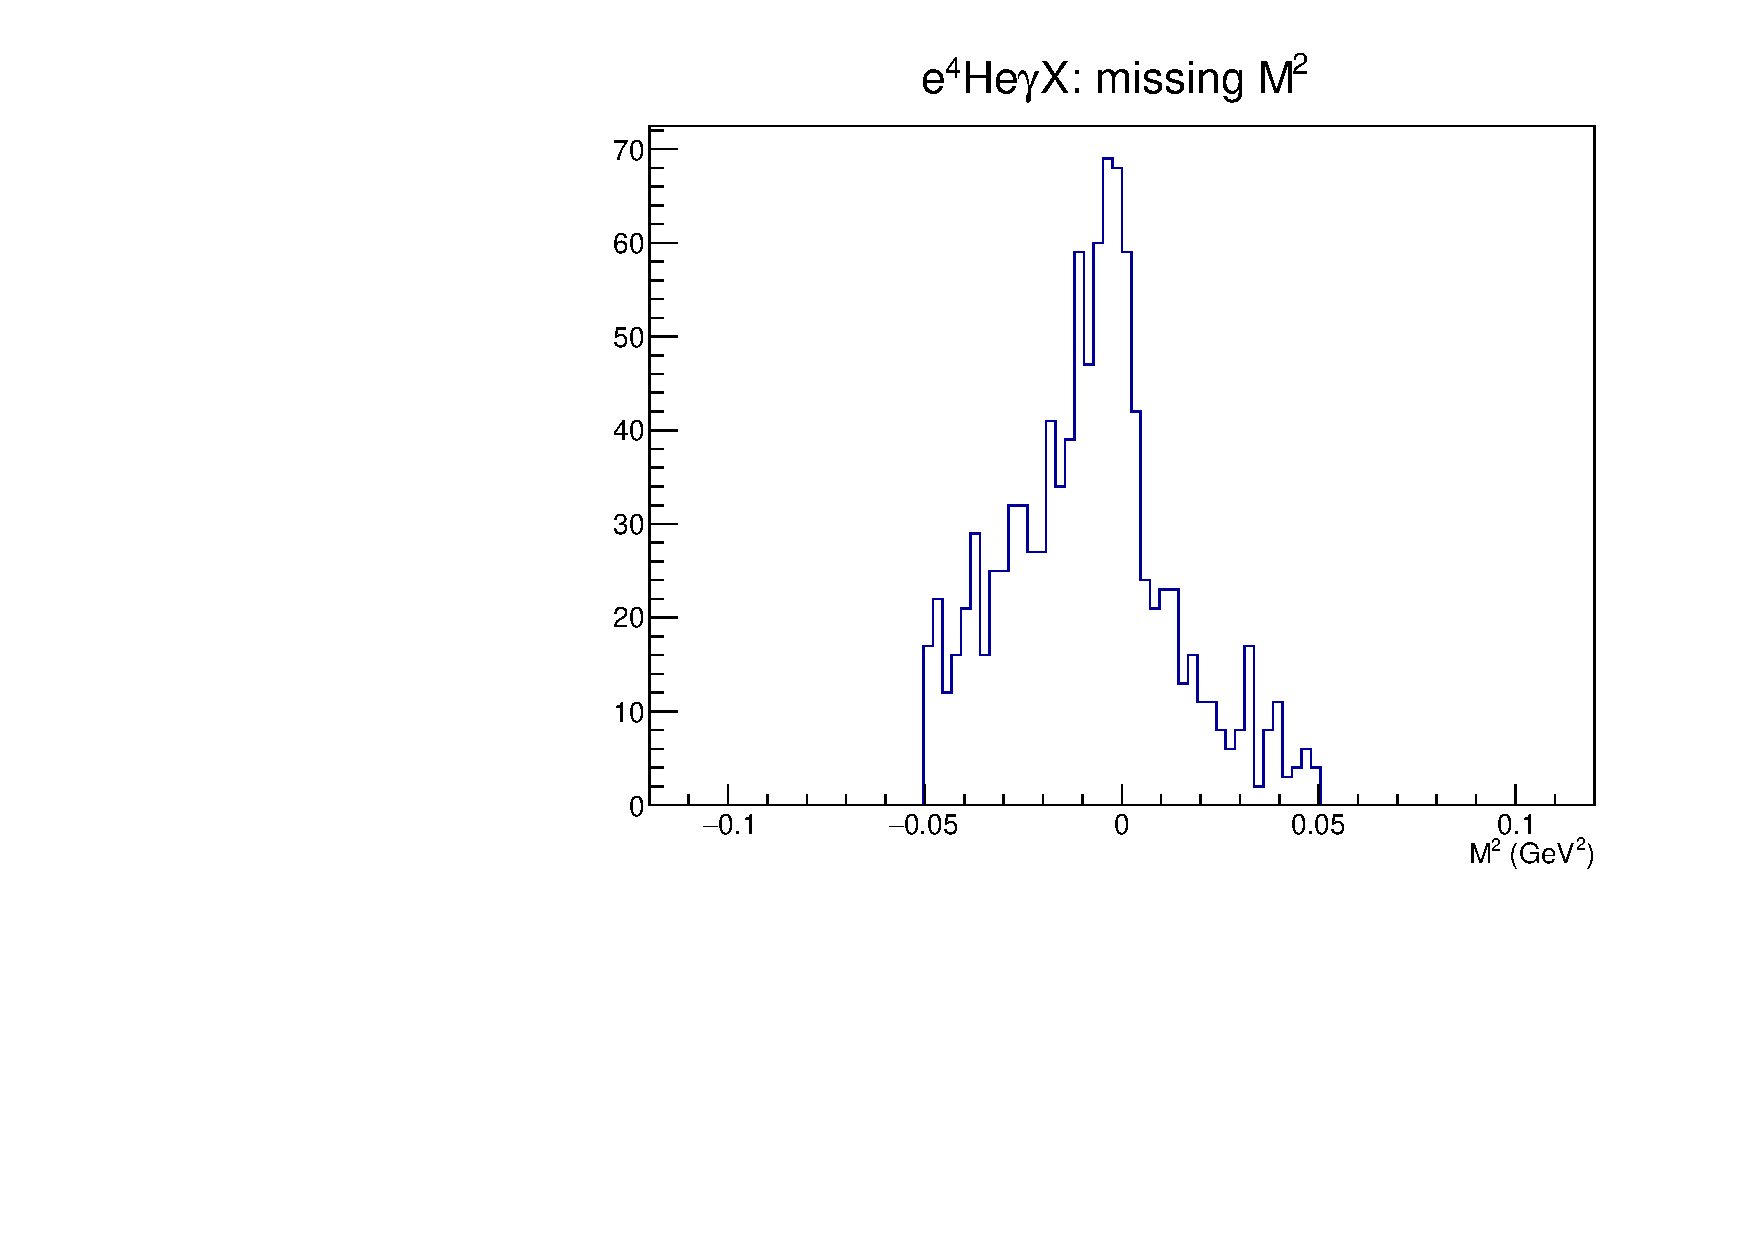
\includegraphics[width=\linewidth]{figures/dvcs_e4HegX_missing_M2.pdf}
    \end{minipage}
    \begin{minipage}{0.3\linewidth}
        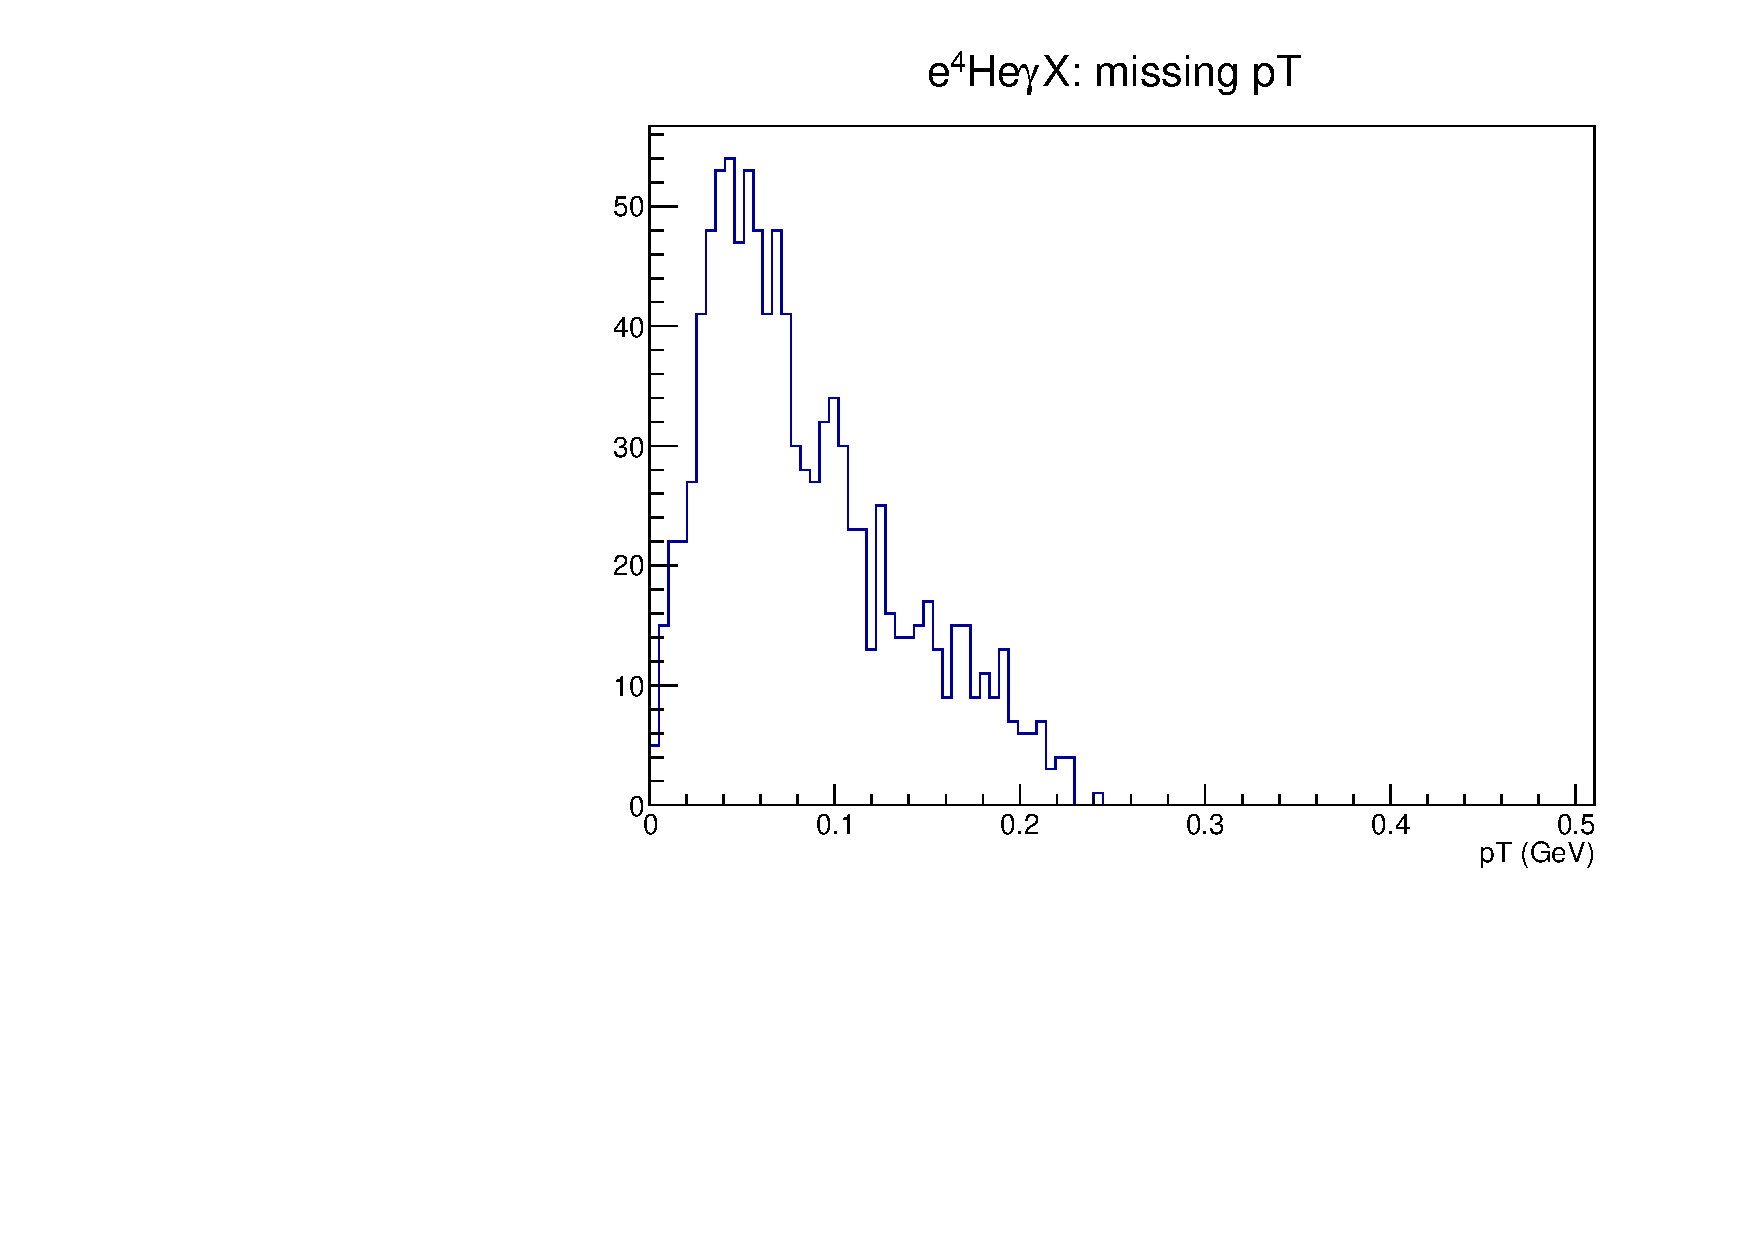
\includegraphics[width=\linewidth]{figures/dvcs_e4HegX_missing_pT.pdf}
    \end{minipage}
    \begin{minipage}{0.3\linewidth}
        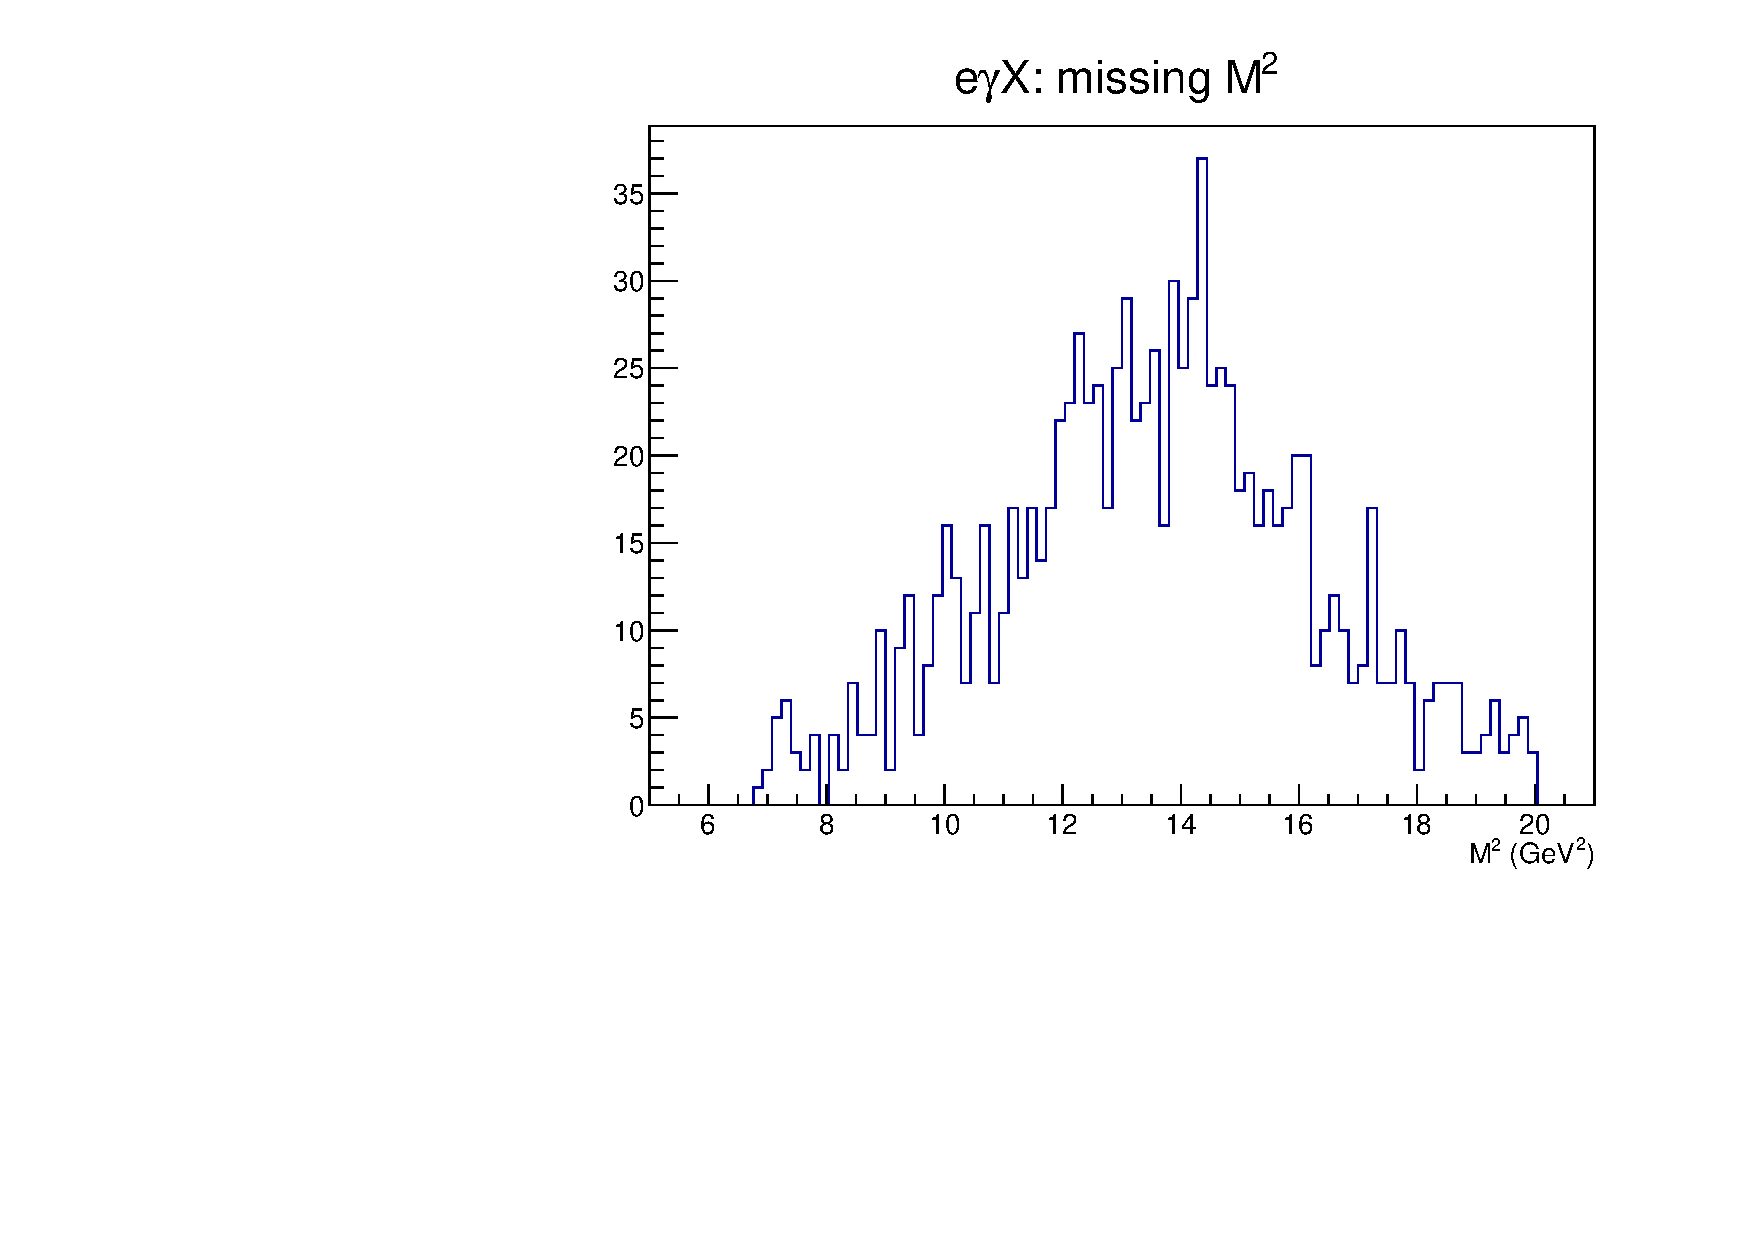
\includegraphics[width=\linewidth]{figures/dvcs_egX_missing_M2.pdf}
    \end{minipage}

    % \begin{minipage}{0.3\linewidth}
    %     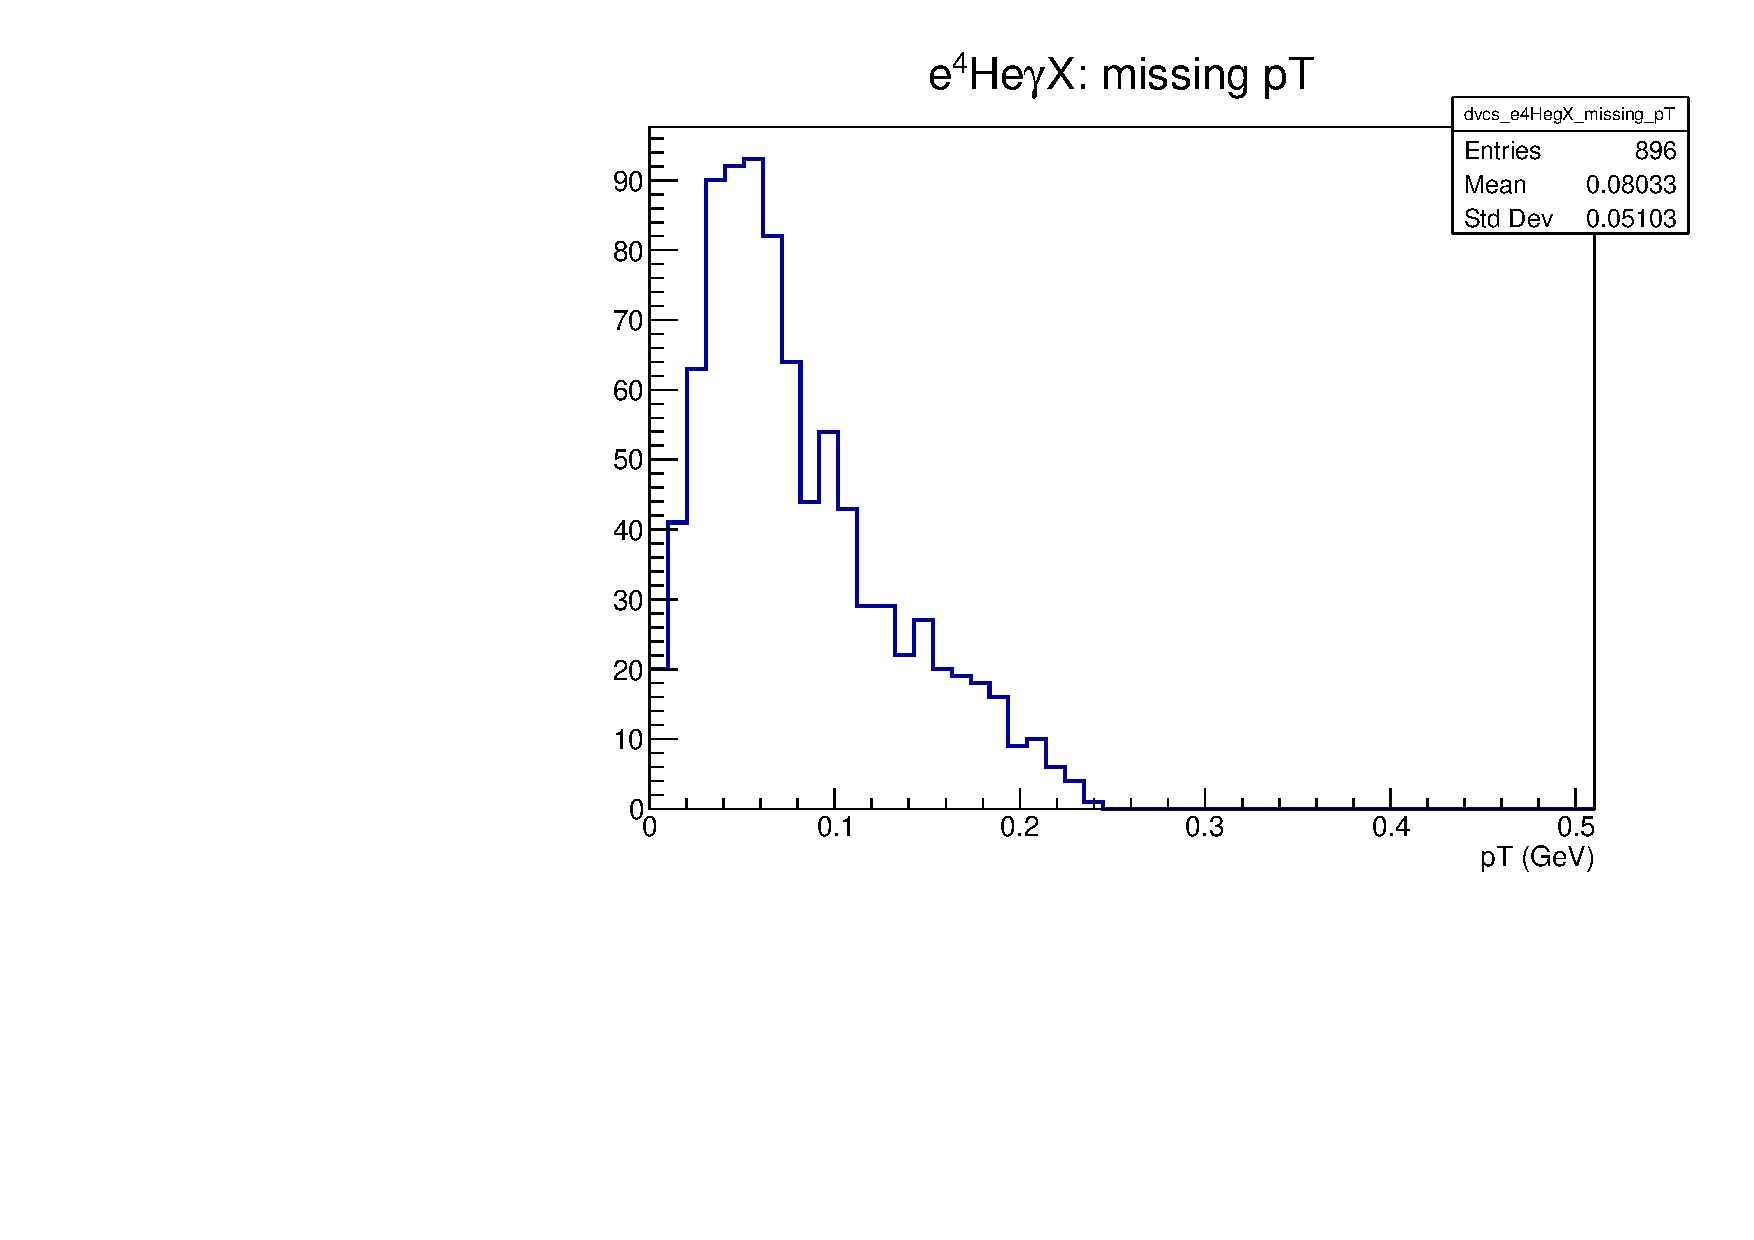
\includegraphics[width=\linewidth]{figures/c_dvcs_e4HegX_missing_pT.pdf}
    % \end{minipage}
    
\end{frame}

\begin{frame}{Phase space}

    \begin{itemize}
        \item $\langle Q^2 \rangle = 1.941 \mbox{ GeV}^2$, $\langle x_B \rangle = 0.137$, $\langle -t \rangle = 0.109 \mbox{ GeV}^2$
    \end{itemize}
    
    \centering
    \vspace{0.2cm}

    \begin{minipage}{0.36\linewidth}
        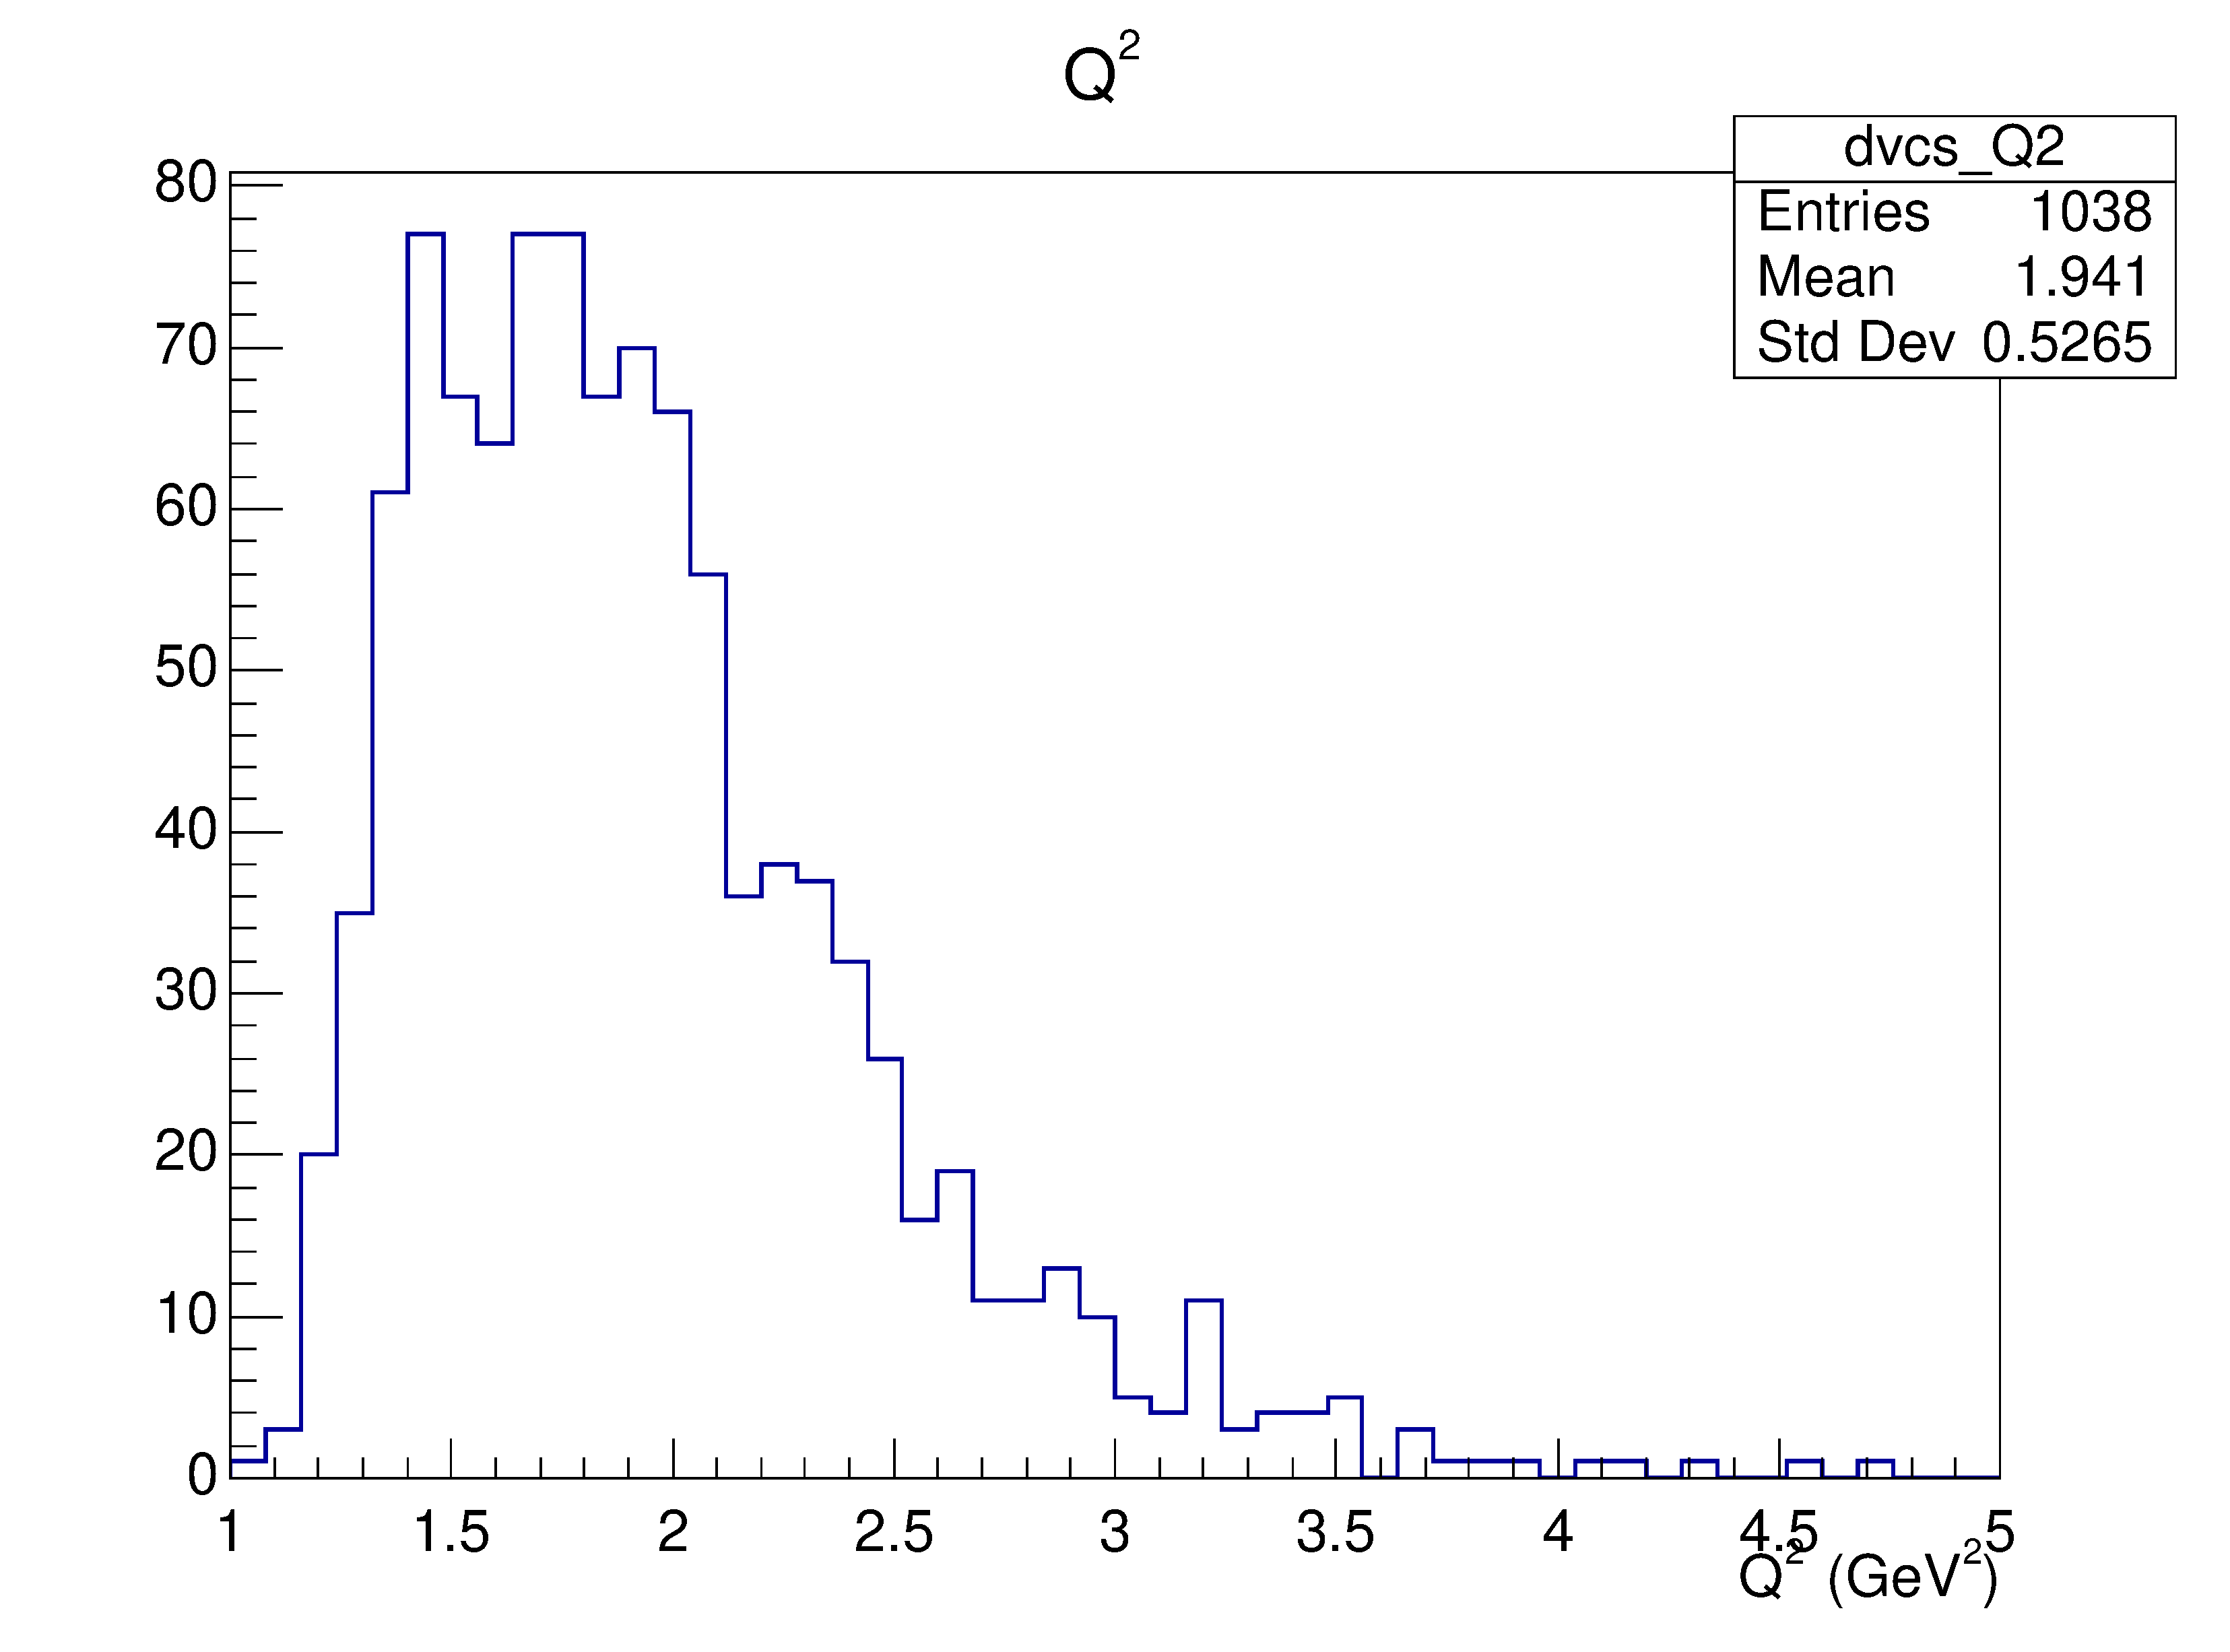
\includegraphics[width=\linewidth]{figures/c_dvcs_Q2.pdf}
    \end{minipage}
    \begin{minipage}{0.36\linewidth}
        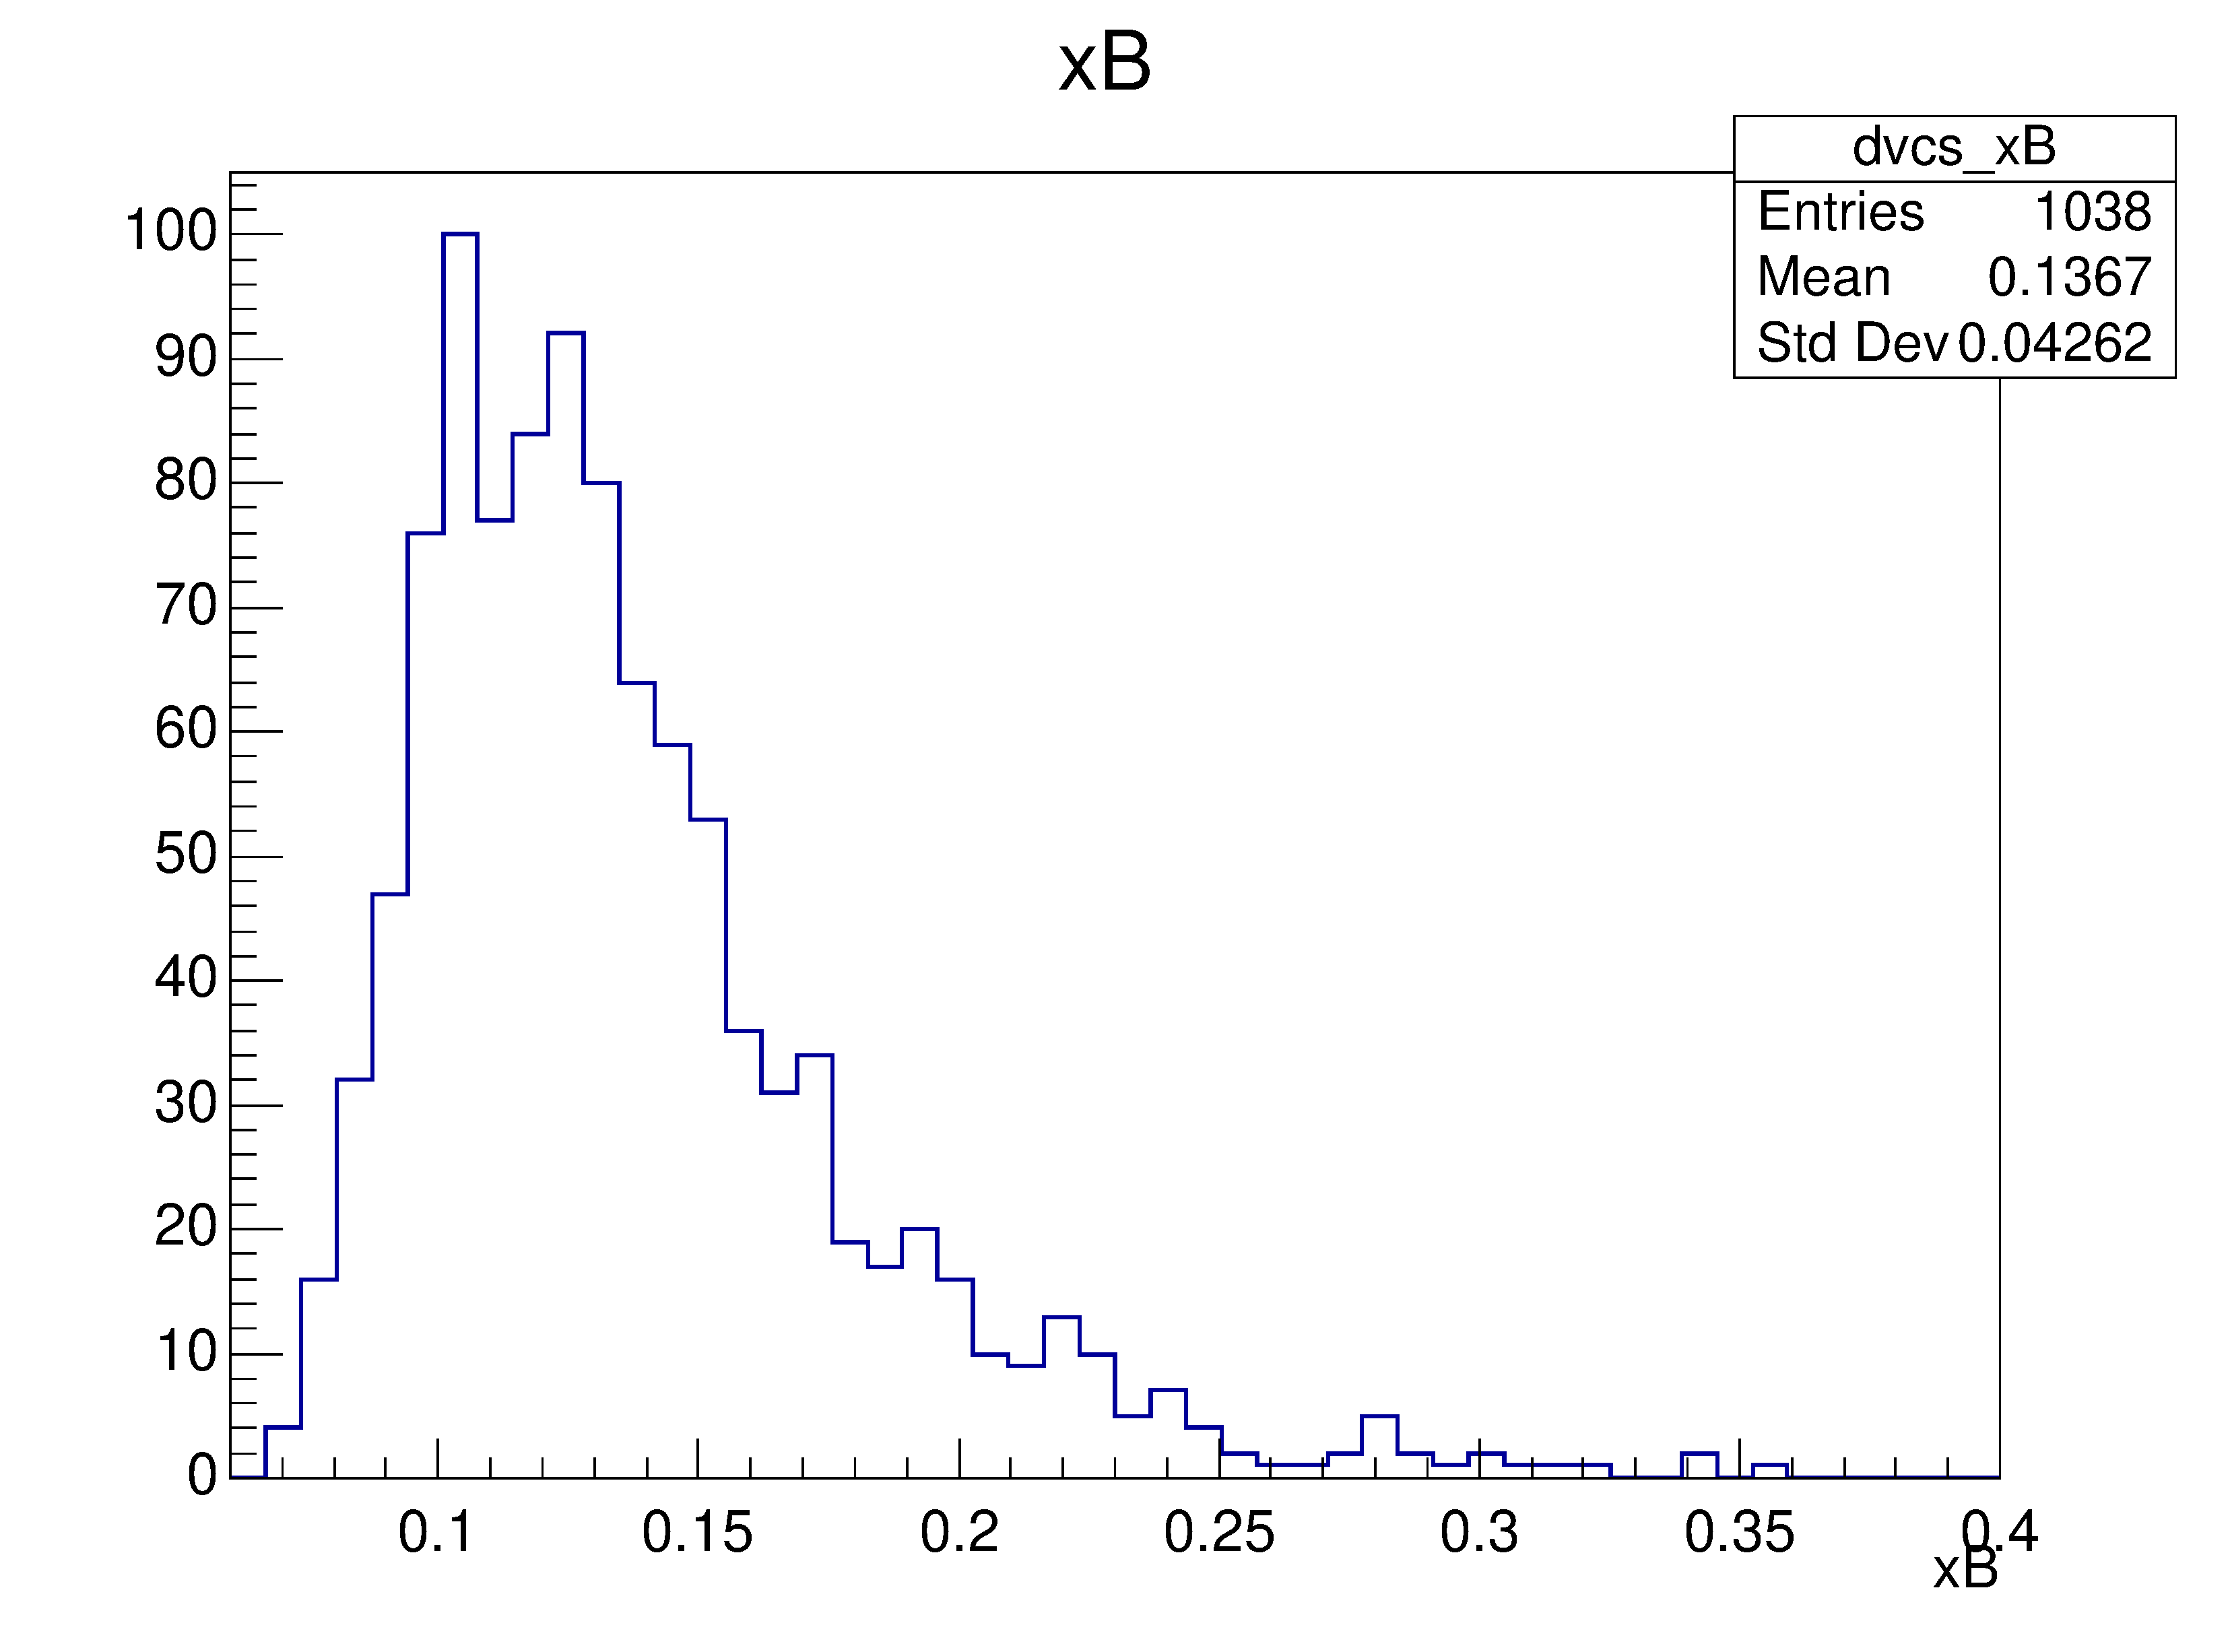
\includegraphics[width=\linewidth]{figures/c_dvcs_xB.pdf}
    \end{minipage}

    \begin{minipage}{0.36\linewidth}
        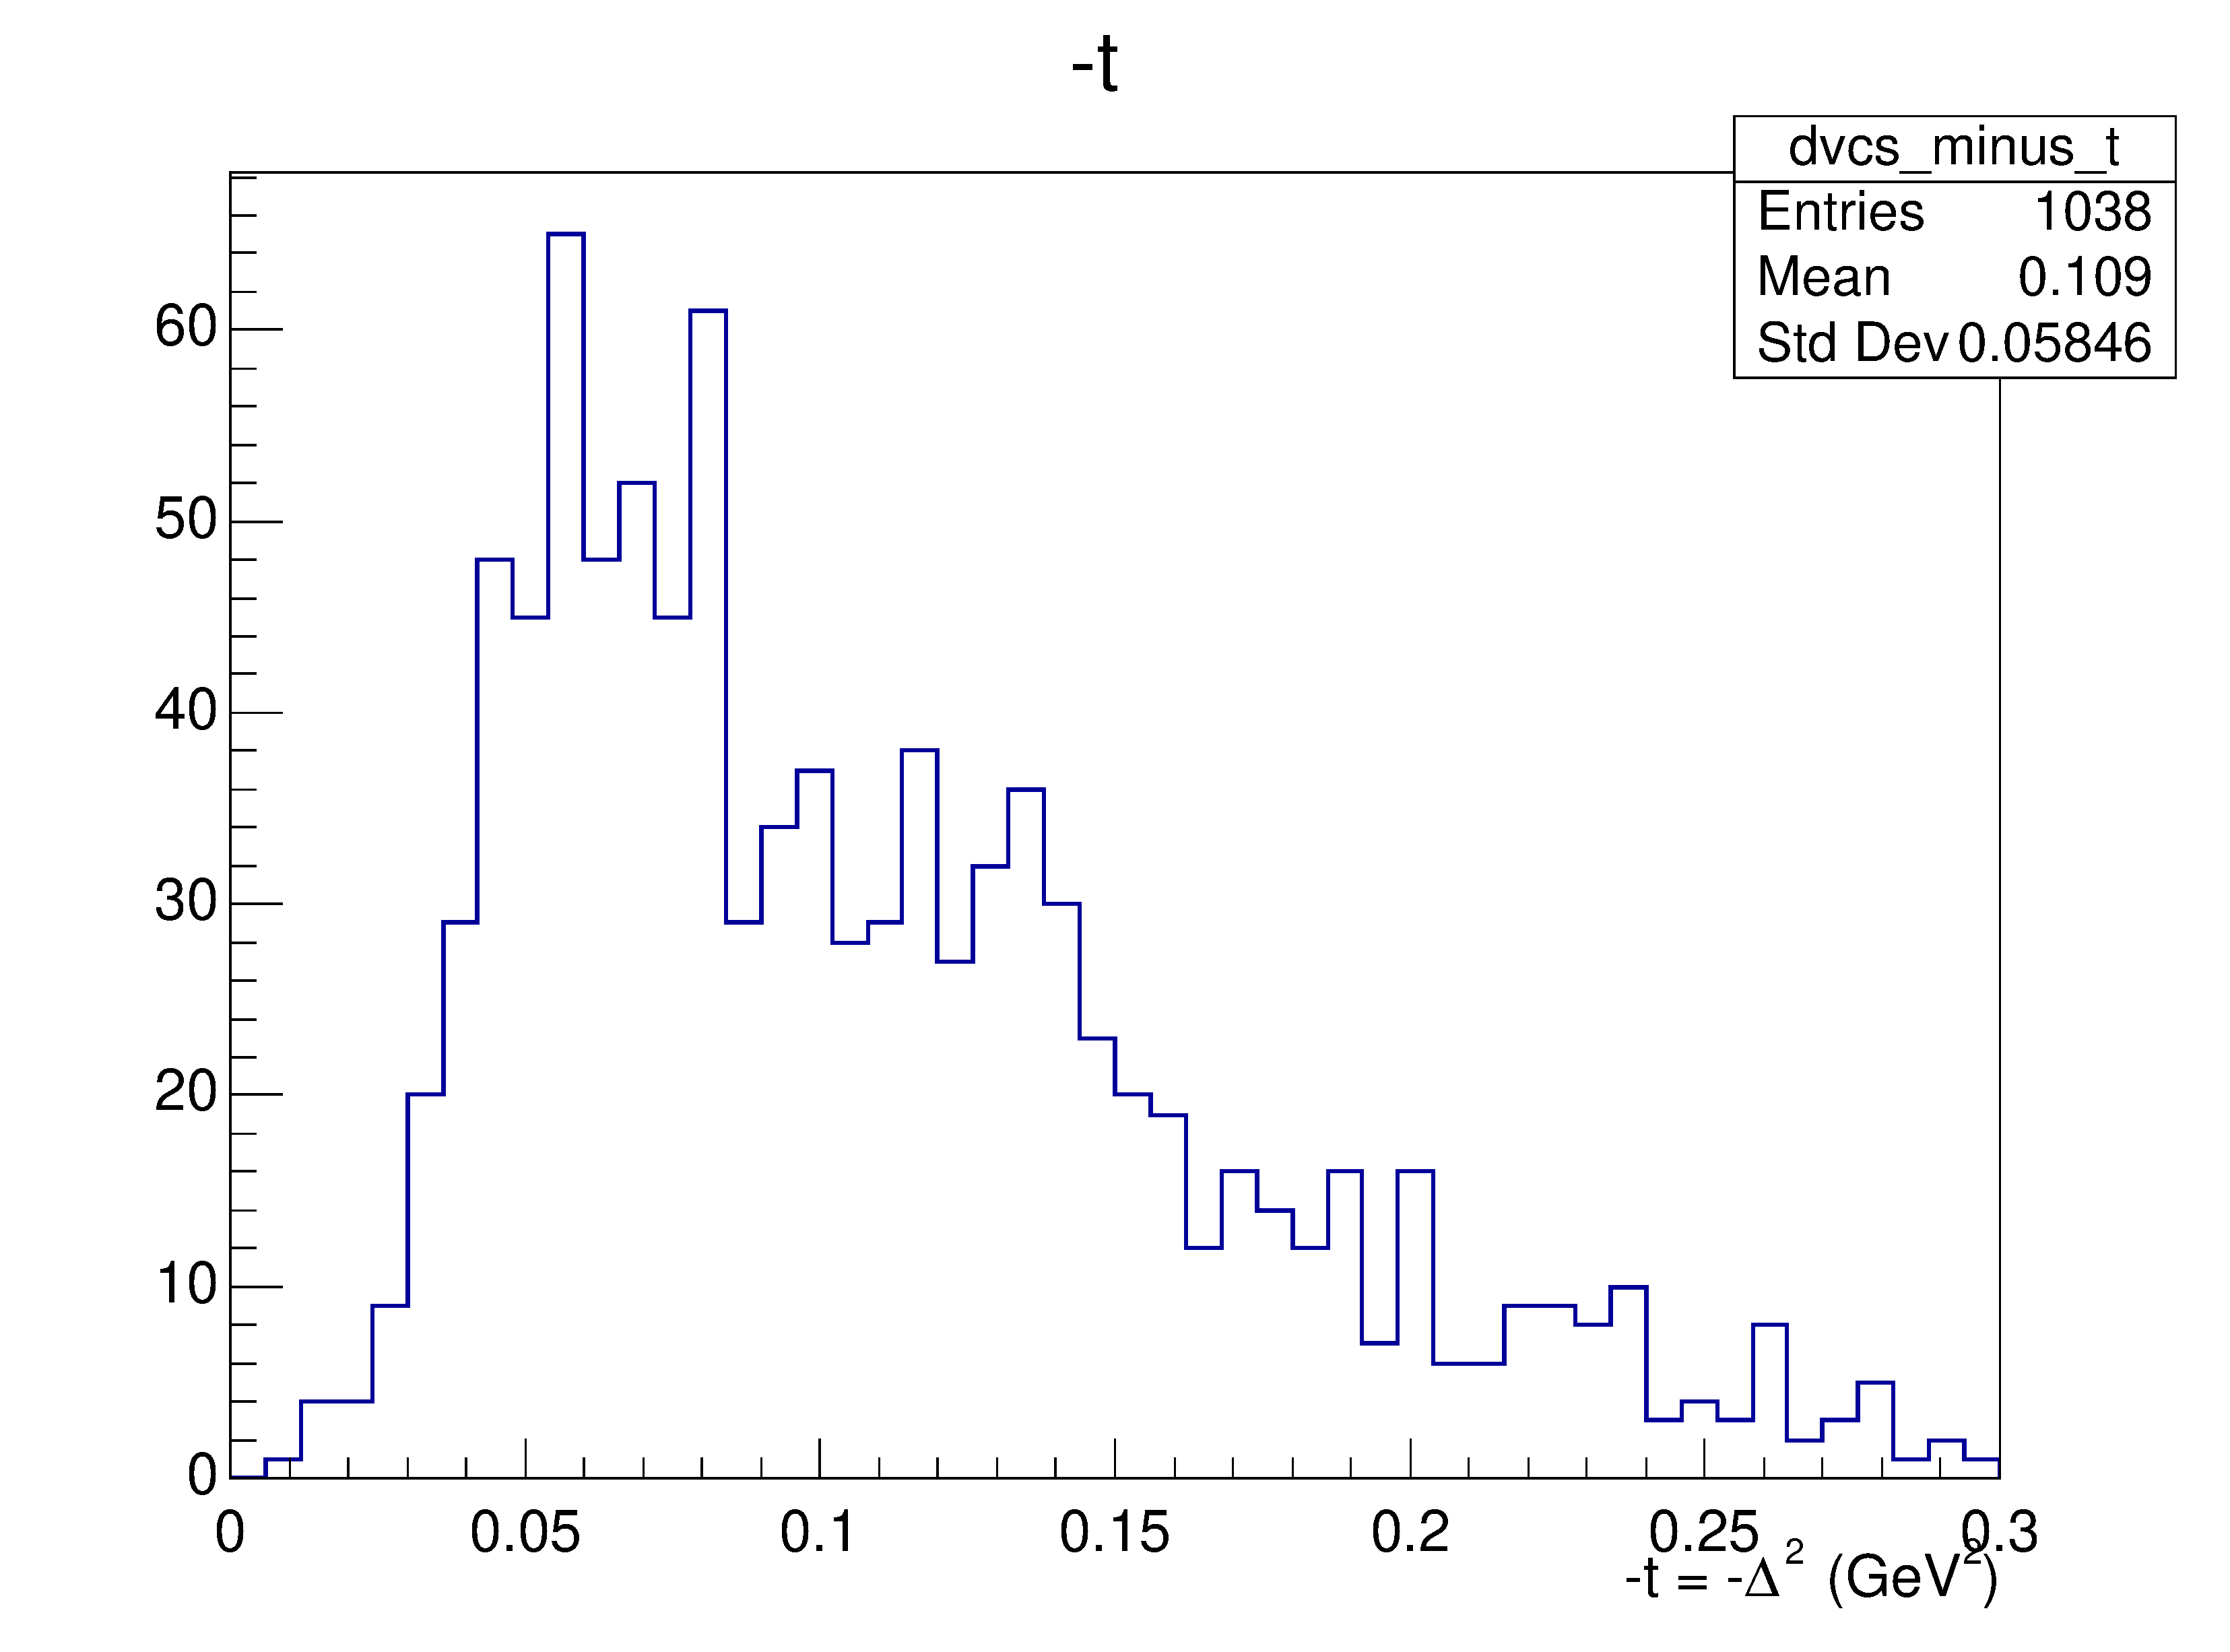
\includegraphics[width=\linewidth]{figures/c_dvcs_minus_t.pdf}
    \end{minipage}
    \begin{minipage}{0.36\linewidth}
        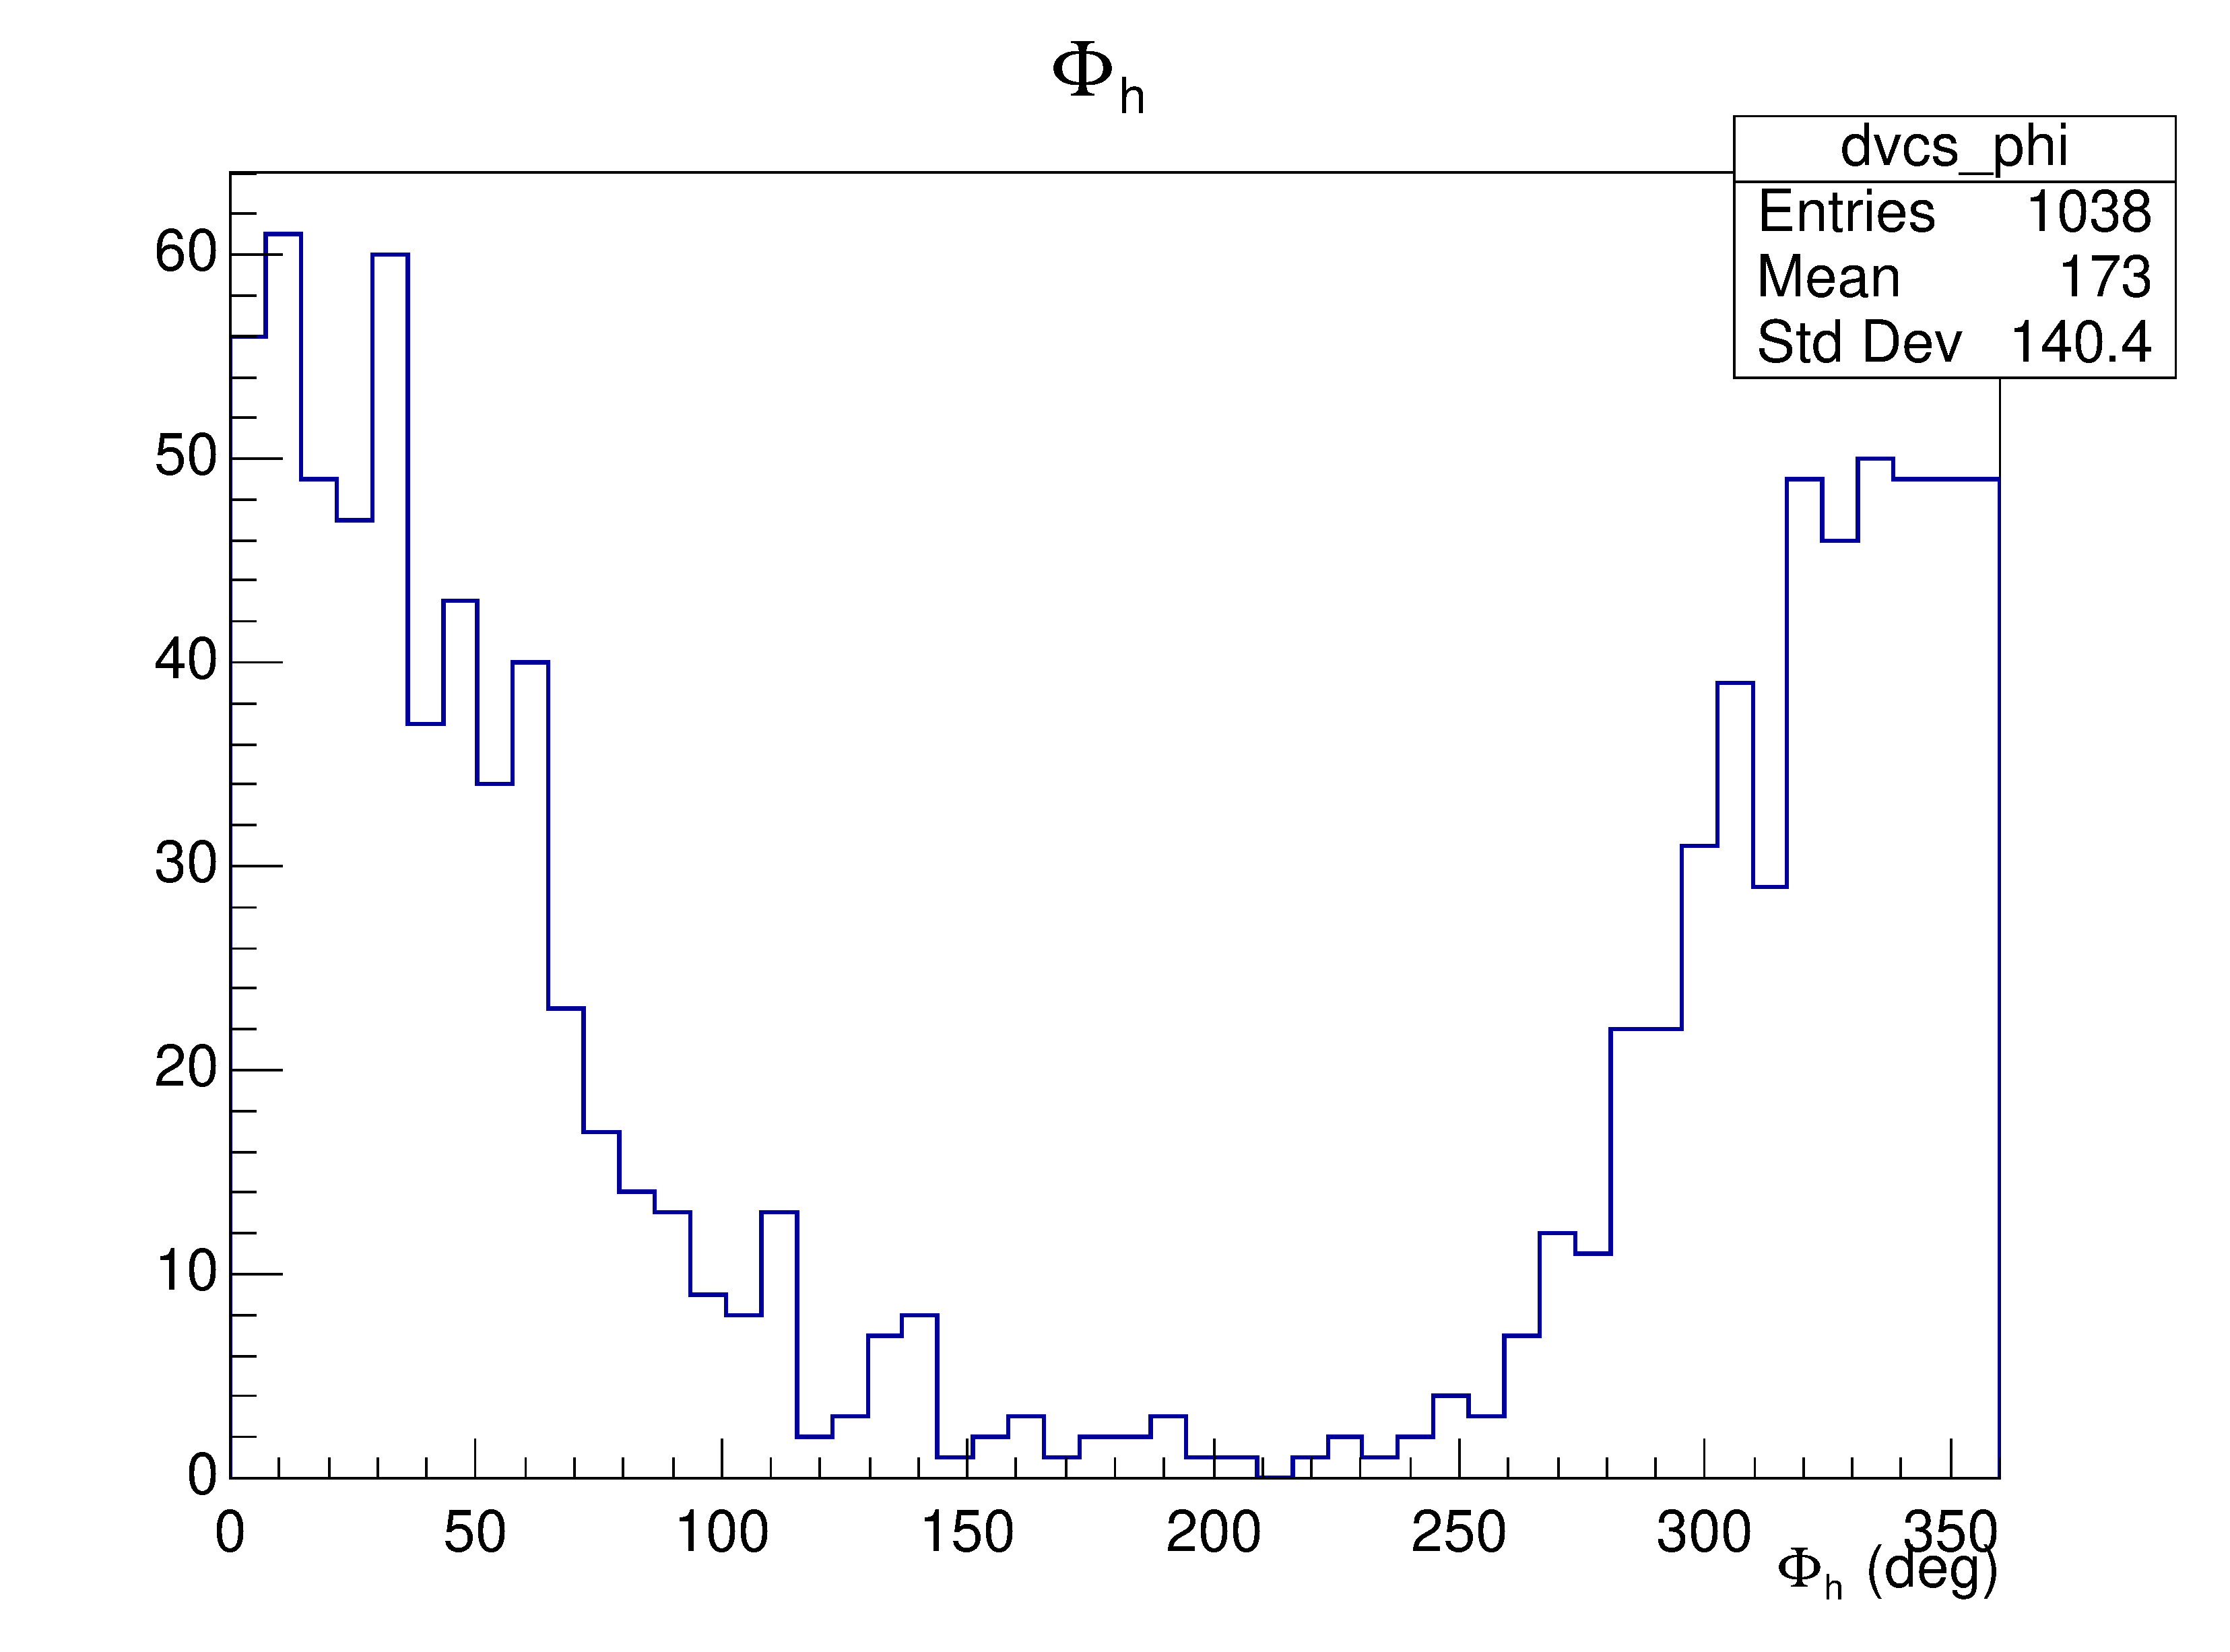
\includegraphics[width=\linewidth]{figures/c_dvcs_phi.pdf}
    \end{minipage}

\end{frame}

\begin{frame}{Preliminary BSA extraction}

    \begin{itemize}
        \item Warnings
            \begin{itemize}
                \item The AHDC reconstruction is not completed (bugs, fine-tuning)
                \item The calibration is still ongoing (ALERT and CLAS)
                \item We made basic selection cuts
                \item The BSA has been integrated over $Q^2$, $x_{B}$ and $-t$
                \item The errors are only statistical (no $\pi ^0$ background subtraction)
            \end{itemize}
        \item The study has been done on 7.53 \% of the data
        \item However, we can already an asymmetry
    \end{itemize}
    

    \centering
    \vspace{0.2cm}

    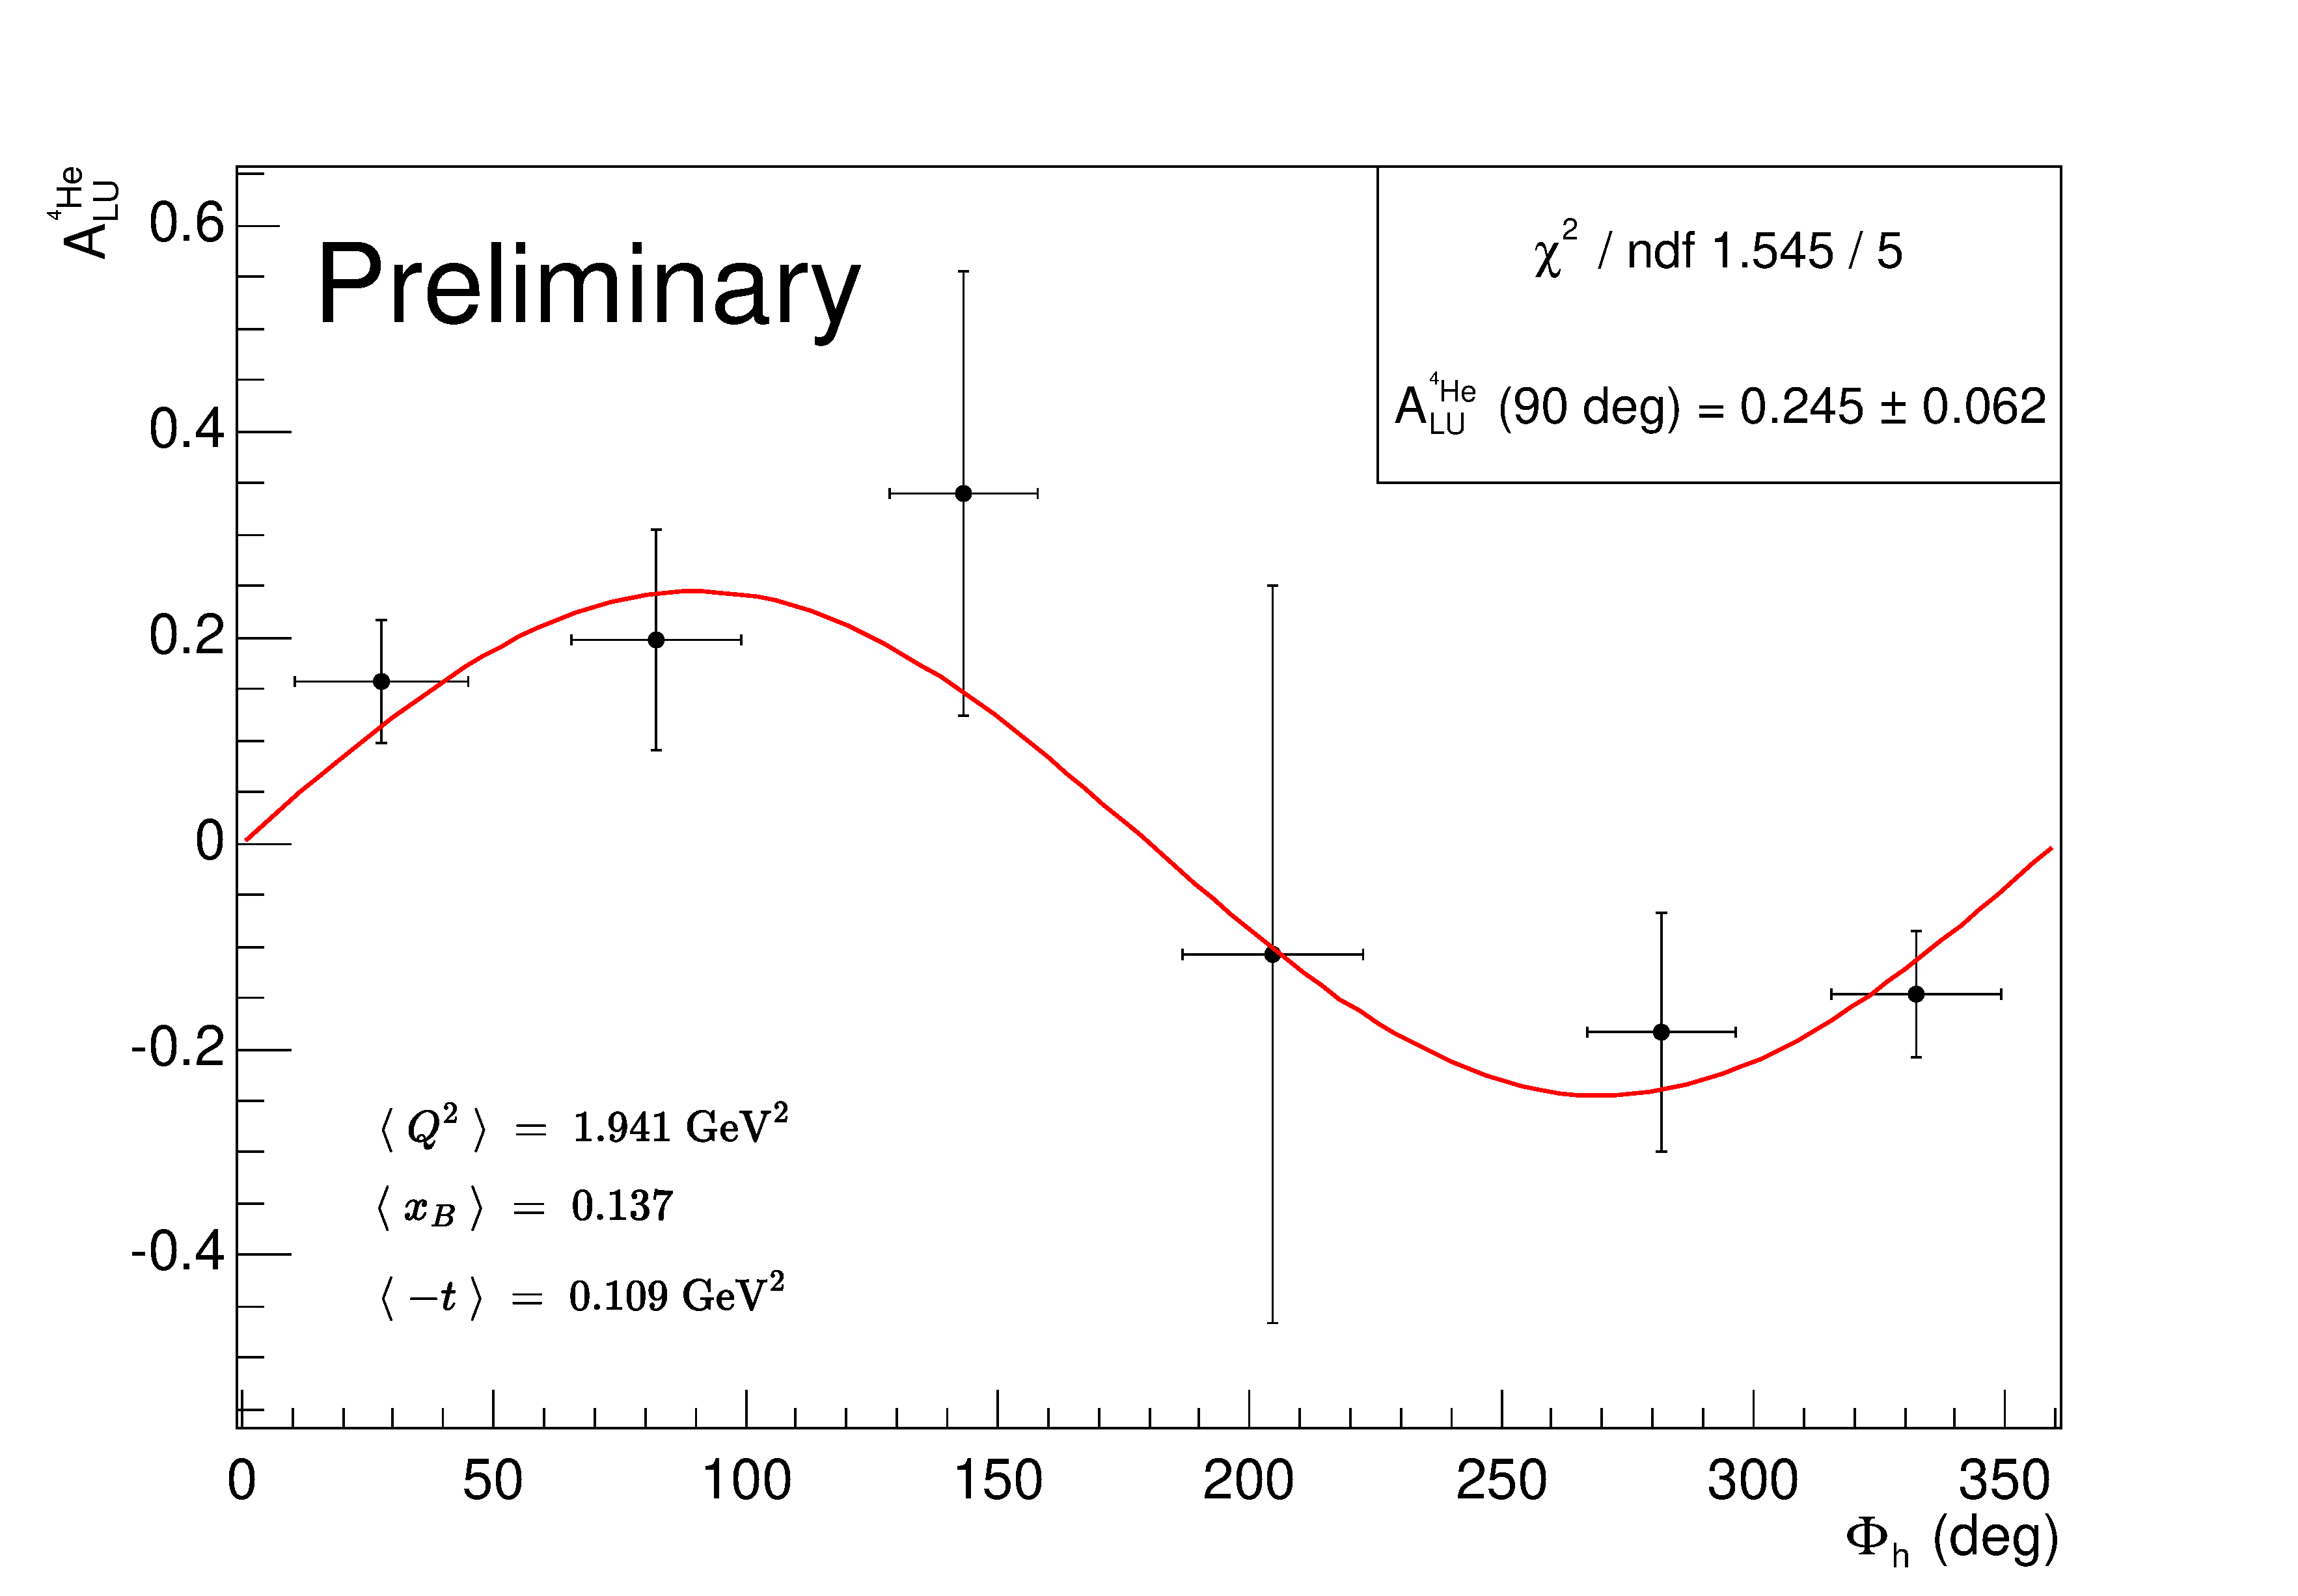
\includegraphics[width=0.55\linewidth]{figures/bsa.pdf}
    
\end{frame}

\begin{frame}{Technical details on the dataset}
    \begin{itemize}
        %\item Study done on October 05, 2026 at 14:20 (UTC +2)
        \item I used p0v12 data from various cooking
            \begin{itemize}
                \item /volatile/clas12/rg-l/production/p0v12/CalibTrain/calib/recon/
                \item /volatile/clas12/rg-l/production/p0v12/FullRuns/calib/recon/
                \item /volatile/clas12/rg-l/production/p0v12/FullNew/calib/recon/
                \item /volatile/clas12/rg-l/production/p0v12/NewRunsforKlest/mon/recon/
            \end{itemize}
        \item List of all runs used : $^4\mbox{He}$ target, 10.6 GeV
        
        21567, 21460, 21638, 21497, 21536, 21517, 21552, 21626, 21610, 21781, 21559, 21627, 21606, 21575, 21472, 21459, 21782, 21481, 21568, 21534, 21533, 21471, 21576, 21520, 21518, 21793, 21794, 21806, 21807, 21855, 21858, 21915, 21919, 21973, 21976, 22522, 22523, 22524, 22526

        \item Corresponding nb evio files : 47995
        \item Total RG-L evio files for $^4\mbox{He}$ target at  10.6 GeV: 637732
        \item {\color{red}Fraction of data used : 7.53 \%}

    \end{itemize}
    
\end{frame}








\end{document}


